% Tratto da grfguide.[ps|pdf]:
%
%\graphicspath{<dir-list>}
%    This optional declaration may be used to specify a list of directories in which to search
%    for graphics files. The format is the same as for the LATEX 2e primitive \input@path.
%    A list of directories, each in a {} group (even if there is only one in the list). For example:
%    \graphicspath{{eps/}{tiff/}}
%    would cause the system to look in the subdirectories eps and tiff of the current directory.
%
%\graphicspath{{FIGS/}}
%
% E` preferibile fare come segue, perche' in questo modo ad es. anche i .tex
% possono essere messi in altre directory e inclusi senza indicarne il percorso.
\makeatletter
\let\input@path=\@undefined
\def\input@path{{FIGS/}}
\makeatother

\ifx\pdfoutput\undefined % We are not running pdftex
\documentclass[12pt,a4paper]{report}

\usepackage[dvips]{graphicx,color}
% \usepackage{psfig}
% \usepackage{epsfig}
\DeclareGraphicsExtensions{.ps,.eps,.pstex}
% Use the following line if you want to obtain a .pdf through dvipdfm
% (.tex -(latex)-> .dvi -(dvipdfm)-> .pdf)
\RequirePackage[dvipdfm,hyperindex]{hyperref}
% % \RequirePackage[dvipdfm,colorlinks,hyperindex]{hyperref}
% Use the following two lines if you want to obtain a .pdf with hyperlinks
% also through ps2pdf (.tex -(latex)-> .dvi -(dvips)-> .ps -(ps2pdf)-> .pdf)
% (this can be useful if you want to use Inkscape and PSFrag to put
%  equations in the figure)
% \RequirePackage[hyperindex]{hyperref}
% \usepackage{psfrag}
% % \RequirePackage[hypertex]{hyperref}
\else % We are running pdftex
\documentclass[pdftex,12pt,a4paper]{report}
\usepackage[pdftex]{graphicx,color}
\DeclareGraphicsExtensions{.pdf,.png,.jpg,.mps}
\RequirePackage[hyperindex]{hyperref}
% % \RequirePackage[colorlinks,hyperindex]{hyperref}
% % \usepackage{thumbpdf}
\hypersetup{
pdftitle={Sperimentazione di reti wireless mobili mediante virtualizzazione container-based ed emulazione in tempo reale del canale},
pdfsubject={Tesi Laurea Magistrale},
pdfauthor={Fabio Di Sabatino},
pdfkeywords={Modello, tesi, LaTeX, PDF, Howto, pdflatex, dvipdfm},
% pdfpagemode=FullScreen
}
\fi

\usepackage{times}
%\usepackage{mathptmx}
\usepackage[scaled=.90]{helvet}
\usepackage{courier}

\textwidth	140 mm
\textheight	210 mm
\headheight	 10 mm
\headsep	  8 mm
\hoffset	 14.6 mm
\oddsidemargin	  0 mm
\voffset	  9.6 mm
\topmargin	  0 mm
\renewcommand{\baselinestretch}{1.14}
% \renewcommand{\baselinestretch}{1}
% \baselineskip = 20 pt

\date{~}
\newlength{\defaultparindent}
\setlength{\defaultparindent}{\parindent}

\usepackage{enumerate}
\usepackage{float}

\usepackage[italian]{babel}
\usepackage[utf8x]{inputenc}
%\usepackage[latin1]{inputenc}
%\usepackage[applemac]{inputenc}

\frenchspacing

\usepackage{amssymb,amstext,amsmath}
%\usepackage{bigint}
%\usepackage{esint}
\usepackage{multirow}
\usepackage{listings}
\usepackage{color}

\newcommand{\ty}{\tilde{y}}
\newcommand{\tM}{\widetilde{M}}
\newcommand{\tSIR}{\text{SIR}}
\newcommand{\tout}{\text{out}}
\newcommand{\thit}{\text{hit}}
\newcommand{\thop}{\text{hop}}
\newcommand{\setawn}{\left( \sigma_{w_n} , \eta_{w_n} \right)}
\newcommand{\var}{\text{var}}
%\def\myvector#1{\underline{#1}}
%\def\myversor#1{\hat{\underline{#1}}}
\newcommand{\myvector}[1]{\underline{#1}}
\newcommand{\myversor}[1]{\hat{\underline{#1}}}
%\newcommand{\myvector}[1]{\text{\boldmath $#1$}}
%\newcommand{\myversor}[1]{\hat{\text{\boldmath $#1$}}}
%\newcommand{\mymatrix}[1]{\text{\boldmath $#1$}}
\newcommand{\mymatrix}[1]{\pmb{#1}}
\newcommand{\erf}{\text{erf}}
\newcommand{\erfc}{\text{erfc}}
\newcommand{\erfinv}{\text{erfinv}}
\newcommand{\inverf}{\text{inverf}}
\newcommand{\rect}{\text{rect}}
\newcommand{\rep}{\text{rep}}
\newcommand{\sinc}{\text{sinc}}
\newcommand{\sgn}{\text{sgn}}
\newcommand{\conv}{\otimes}
\newcommand{\T}{\mathbb{T}}
\newcommand{\R}{\mathbb{R}}
\newcommand{\Z}{\mathbb{Z}}
\newcommand{\C}{\mathbb{C}}
\newcommand{\F}{\mathcal{F}}

\RequirePackage{fancyhdr}
\pagestyle{fancy}
\fancyhf{}
%\renewcommand{\chaptermark}[1]{\markboth{\scshape \chaptername\ \thechapter\ -- #1}{}}
\renewcommand{\chaptermark}[1]{\markboth{\chaptername\ \thechapter\ -- #1}{}}
\fancyhead[L]{\leftmark}
\fancyhead[R]{\thepage}

% Per far numerare anche le subsubsection:
\setcounter{secnumdepth}{3} % il default è 2 e quindi comprende fino alle subsection
% Per far inserire anche le subsubsection nella Table Of Contents:
\setcounter{tocdepth}{3}    % il default è 2 e quindi comprende fino alle subsection
\usepackage[normal]{subfigure}

\usepackage{verbatim}

%%MY STYLES
%%%%%%%%%%%
%%  XML  %%
%%%%%%%%%%%
\definecolor{gray}{rgb}{0.4,0.4,0.4}
\definecolor{darkblue}{rgb}{0.0,0.0,0.6}
\definecolor{cyan}{rgb}{0.0,0.6,0.6}
\DeclareFixedFont{\ttb}{T1}{txtt}{bx}{n}{12} % for bold
\DeclareFixedFont{\ttm}{T1}{txtt}{m}{n}{12}  % for normal
\definecolor{deepblue}{rgb}{0,0,0.5}
\definecolor{deepred}{rgb}{0.6,0,0}
\definecolor{deepyellow}{rgb}{0.6,0.6,0}
\definecolor{deepgreen}{rgb}{0,0.5,0}

\lstset{
  basicstyle=\ttfamily,
  columns=fullflexible,
  showstringspaces=false,
  commentstyle=\color{gray}\upshape,
  breaklines=true,
}

\lstdefinelanguage{XML}
{
  morestring=[b]",
  morestring=[s]{>}{<},
  morecomment=[s]{<?}{?>},
  stringstyle=\color{black},
  identifierstyle=\color{darkblue},
  keywordstyle=\color{cyan},
  morekeywords={xmlns,version,type}% list your attributes here
}
\lstdefinelanguage{JavaScript}{
  keywords={typeof, new, true, false, catch, function, return, null, catch, switch, var, if, in, while, do, else, case, break},
  keywordstyle=\color{blue}\bfseries,
  ndkeywords={class, export, boolean, throw, implements, import, this},
  ndkeywordstyle=\color{darkblue}\bfseries,
  identifierstyle=\color{black},
  sensitive=false,
  comment=[l]{//},
  morecomment=[s]{/*}{*/},
  commentstyle=\color{red}\ttfamily,
  stringstyle=\color{red}\ttfamily,
  morestring=[b]",
}
%%%%%%%%%%%
%%  PHP  %%
%%%%%%%%%%%
\lstdefinelanguage{PHP}
{
  morestring=[b]",
  morestring=[s]{"}{"},
  stringstyle     =\color{deepgreen},
  identifierstyle =\color{black},
  otherkeywords   = {fopen, fclose, bcadd, fwrite, bccomp, bcsub, true, false, ksort, isset, fgets, round, substr, preg_match, feof, trim, explode},   
  keywordstyle    =\color{darkblue},
  commentstyle    = \color{gray},
  emph            =[1]{php, <?php, ?>},
  emphstyle       =[1]\color{black},
  emph            =[2]{if,and,or,else,while,for, foreach, as},
  emphstyle       =[2]\color{deepred}
}

%%%%%%%%%%%%
%%  BASH  %%
%%%%%%%%%%%%
\lstdefinelanguage{BASH}
{
  stringstyle=\color{black},
  identifierstyle=\color{darkblue},
  commentstyle=\color{red},
  keywordstyle=\color{blue},
  morekeywords={xmlns,version,type}% list your attributes here
}

%%%%%%%%%%%%
%% PYTHON %%
%%%%%%%%%%%%
\lstdefinelanguage{PYTHON}
{
  morestring=[s]{"}{"},
  stringstyle=\color{deepgreen},
  identifierstyle =\color{black},
  basicstyle=\ttm,
  otherkeywords={self, import, def, class, except, open, while, str, handle.write, handle.close},             % Add keywords here
  keywordstyle=\ttb\color{deepblue},
  emph={MyClass,__init__},          % Custom highlighting
  emphstyle=\ttb\color{deepred},    % Custom highlighting style
  frame=tb,                         % Any extra options here
  showstringspaces=false,           % 
}

\begin{document}

\renewcommand{\figurename}{\small Figura}
\renewcommand{\tablename}{\small Tabella}

% BEGIN Frontespizio
%\begin{titlepage}

\begin{center}
\normalsize

\begin{center}
\begin{tabular}[t]{@{} l @{} c @{} r @{}}
\parbox[c]{0.15\textwidth}{\raggedright 
\includegraphics[width=0.60in]{logo_univ}}
&
\parbox[c]{0.7\textwidth}
{
\centering \bfseries
UNIVERSITÀ DEGLI STUDI DELL'AQUILA \\[-5pt]
\rule{0.65\textwidth}{1pt} \\
{\scshape DIPARTIMENTO DI \\ INGEGNERIA E SCIENZE DELL'INFORMAZIONE E MATEMATICA }
}
&
\parbox[c]{0.15\textwidth}{\raggedleft 
\includegraphics[width=0.70in]{logo_ing}}
\end{tabular}
\end{center}

\bigskip \bigskip



\bigskip \bigskip

{\small CORSO DI LAUREA IN} \\
INGEGNERIA INFORMATICA E AUTOMATICA

\vfil \vfil \vfil

{\bfseries \large
Realizzazione di un sistema di stima dell'assetto mediante IMU sensor fusion
per un'applicazione RTLS indoor\\
}

\vfil \vfil \vfil

\makebox[\textwidth][c]{

\begin{minipage}[t]{0.4\textwidth}
\centering
{\bfseries Relatore:} \\
{\itshape Prof.\ Luigi Pomante} \\
\bigskip
%\dotfill
\underline{\hspace{\textwidth}}
\\
\bigskip \bigskip
{\bfseries Co--relatori:} \\
{\itshape\ Giacomo Valente, Marco Santic} \\
\bigskip
\underline{\hspace{\textwidth}}
\\
\end{minipage}

%\hfil
\hspace*{0.1\textwidth}

\begin{minipage}[t]{0.4\textwidth}
\centering
{\bfseries Candidato:} \\
{\itshape Fabio Di Sabatino} \\
\bigskip
\underline{\hspace{\textwidth}}
\\
\bigskip \bigskip
{\bfseries Matricola:} \\
{\itshape 246526} \\
\bigskip
\underline{\hspace{\textwidth}}
\\
\end{minipage}

}

\vfil \vfil \vfil

\rule{\textwidth}{1pt}\\
{\scshape Anno Accademico 2015--2016}

\end{center}

\end{titlepage}


% END Frontespizio

% BEGIN Pagina di dedica
%\thispagestyle{empty}
\vspace*{5cm}
\parbox[r]{0.95\textwidth}{
\itshape
\raggedleft
Dedico il presente lavoro
\\
a tutte le persone che mi sono
\\
state vicine durante questi anni
}
% END Pagina di dedica

%\newpage

% BEGIN Indice
%\thispagestyle{empty}
\setcounter{page}{1}
\pagenumbering{roman}
\tableofcontents
% END Indice

\newpage

\listoffigures

\newpage

\setcounter{page}{1}
\pagenumbering{arabic}

%\chapter*{Sommario}
\markboth{Sommario}{Sommario}
\addcontentsline{toc}{chapter}{Sommario}
\thispagestyle{empty}

Lo scopo di questa tesi è lo sviluppo di un sistema per la stima dell'assetto di un'operatore in ambienti indoor privi del segnale GPS.\\
Il sistema deve essere in grado di stimare gli angoli assunti dall'operatore nel tragitto che egli effettua per raggiungere la persona da soccorrere; queste informazioni verranno poi utilizzate da un sistema più grande, che esula dal lavoro di questa tesi, al fine di creare una rete di nodi all'interno della quale 
si è in grado di localizzare e guidare i soccorritori.\\
Per realizzare questo sistema si è utilizzato un microcontrollore della STM con processore ARM-Cortex M4, un'unità di misura inerziale della STM dotato di giroscopio accelerometro e magnetometro e l'applicativo Matlab.\\
Per stimare l'assetto si utilizzano due algoritmi di \textit{sensor fusion}; uno trovato in letteratura ed implementato sull'applicativo Matlab, un altro facente parte di una libreria appositamente sviluppata da STM per i processori di questa famiglia.
\\
\\

\noindent
\begin{Huge}
\textbf{Abstract}
\end{Huge}
\\
\\
\noindent
The aim of this thesis is the development of a system for estimating the attitude of an operator in indoor environments where the GPS signal is lacking.
The system must be able to estimate the angles assumed by the operator during the path done to reach the person who has to be rescued; this information will then be used by a larger system, which fall outside the work of this thesis, in order to create a network of nodes within which
it is possible to locate and drive rescuers for the whole time of their operations. \\
To realize this system, it was used a microcontroller by STM with ARM-Cortex M4 processor, an inertial measurement unit by STM equipped with an accelerometer gyroscope and a magnetometer and the Matlab application.
To estimate the attitude two algorithms of \ textit {sensor fusion} are used; one found in the literature and implemented on the Matlab application, another one  which belongs to a library specially developed by STM for the processors of this family.


% !TeX spellcheck = it
\chapter*{Introduzione}
\markboth{Introduzione}{Introduzione}
\addcontentsline{toc}{chapter}{Introduzione}
\thispagestyle{empty}

Il lavoro di questa tesi si colloca nel progetto aziendale Tekne per la realizzazione di un sistema di geolocalizzazione di operatori in contesti privi di segnale GPS.
Il sistema permette ad un “esploratore” di creare dinamicamente una rete di nodi all’interno di zone nelle quali il segnale GPS è assente o comunque debole. Questa rete verrà poi ampliata ed utilizzata dagli operatori successivi ad esso per geolocalizzarsi all’interno della zona ed intervenire in maniera ottimale. \\
Uno scenario esemplificativo è quello di un vigile del fuoco che interviene in un edificio per soccorrere una persona. Tale operatore è considerato un esploratore, poiché è il primo ad intervenire e la planimetria dell’edificio risulta essere ignota e/o cambiata a seguito dell’evento disastroso (Fig.\ref{fig:planOriginale} e Fig.\ref{fig:planAlterata}). 

\begin{figure}[h]
	\begin{minipage}[b]{6cm}
		\centering
		\includegraphics[scale=0.35]{Introduzione/piantina1.png}
		\caption{Planimetria originale}
		\label{fig:planOriginale}
	\end{minipage}
	\ \hspace{10 mm} \
	\begin{minipage}[b]{6cm}
		\centering
		\includegraphics[scale=0.35]{Introduzione/piantina2.png}
		\caption{Planimetria alterata}
		\label{fig:planAlterata}
	\end{minipage}
\end{figure}

\newpage
I rettangoli in grigio (Fig.\ref{fig:planAlterata}) rappresentano aree non più accessibili dell’edificio, mentre le mura interrotte nuovi percorsi creati a causa dei crolli. 
Durante tutta la fase di scouting, l’esploratore posizionerà un’ancora (nodo) ogni 20 metri approsimativamente e ogni qualvolta la precedente risulti non essere più in line-of-sight (linea visiva). Così facendo si “lascerà dietro una scia di briciole” che gli permetteranno di orientarsi all’interno dell’edificio, di eseguire il percorso all’inverso o di ricevere supporto da un’ulteriore operatore. Nelle figure seguenti, si può notare come la rete cresca man mano che l'esploratore avanza all'interno dell'edificio.

\begin{figure}[h]
	\begin{minipage}[b]{6cm}
		\centering
		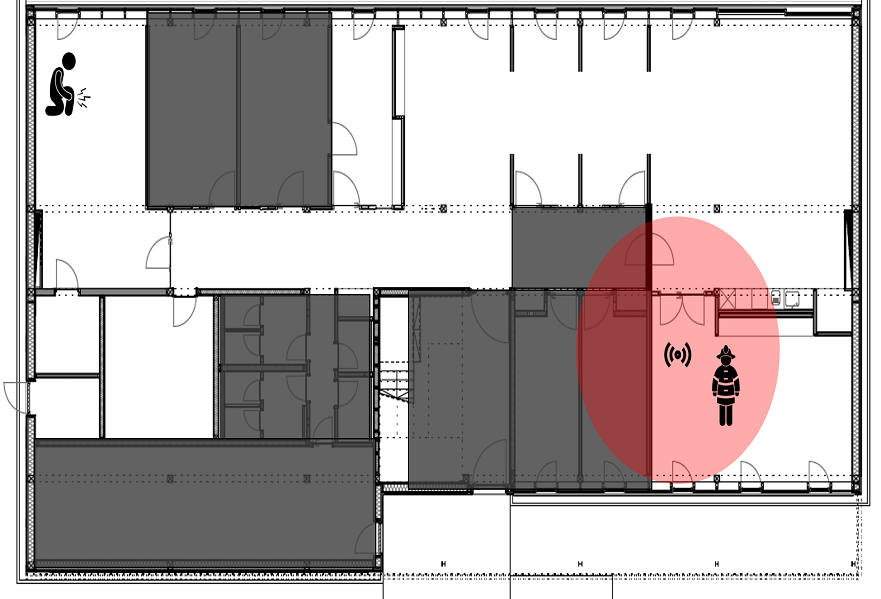
\includegraphics[scale=0.35]{Introduzione/intervento_step_1.png}
		\caption{Rete allo step 1 dell'esploratore}
		\label{fig:step1}
	\end{minipage}
	\ \hspace{10 mm} \
	\begin{minipage}[b]{6cm}
		\centering
		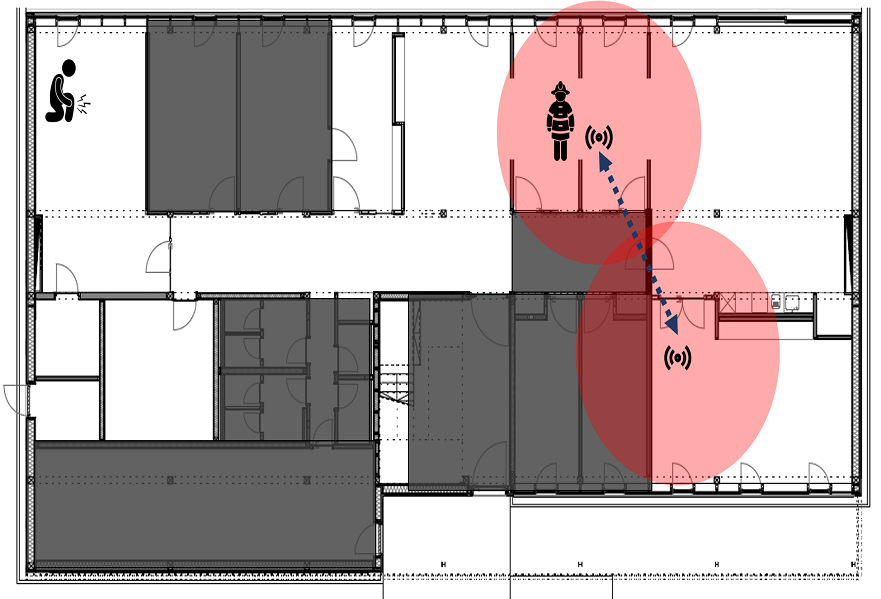
\includegraphics[scale=0.35]{Introduzione/intervento_step_2.png}
		\caption{Rete allo step 1 dell'esploratore}
		\label{fig:step2}
	\end{minipage}
\end{figure}


\begin{figure}[h]
	\begin{minipage}[b]{6cm}
		\centering
		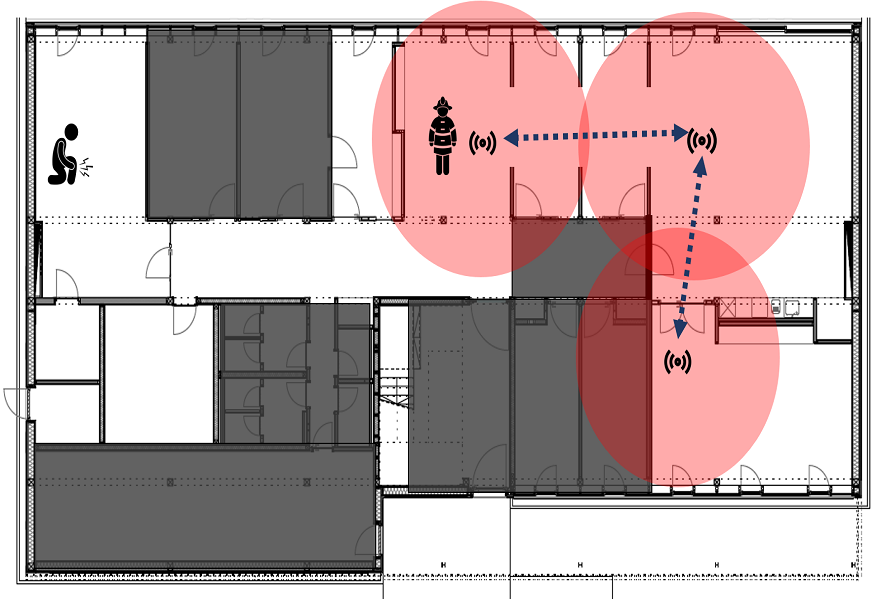
\includegraphics[scale=0.35]{Introduzione/intervento_step_3.png}
		\caption{Rete allo step 3 dell'esploratore}
		\label{fig:step3}
	\end{minipage}
	\ \hspace{10 mm} \
	\begin{minipage}[b]{6cm}
		\centering
		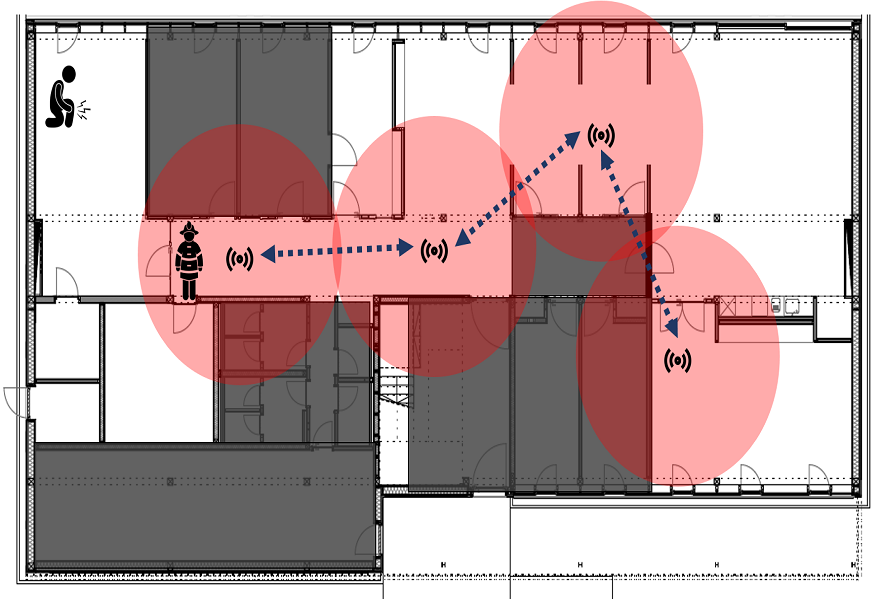
\includegraphics[scale=0.35]{Introduzione/intervento_step_4.png}
		\caption{Rete allo step 4 dell'esploratore}
		\label{fig:step4}
	\end{minipage}
\end{figure}

\begin{figure}[h]
	\begin{minipage}[b]{6cm}
		\centering
		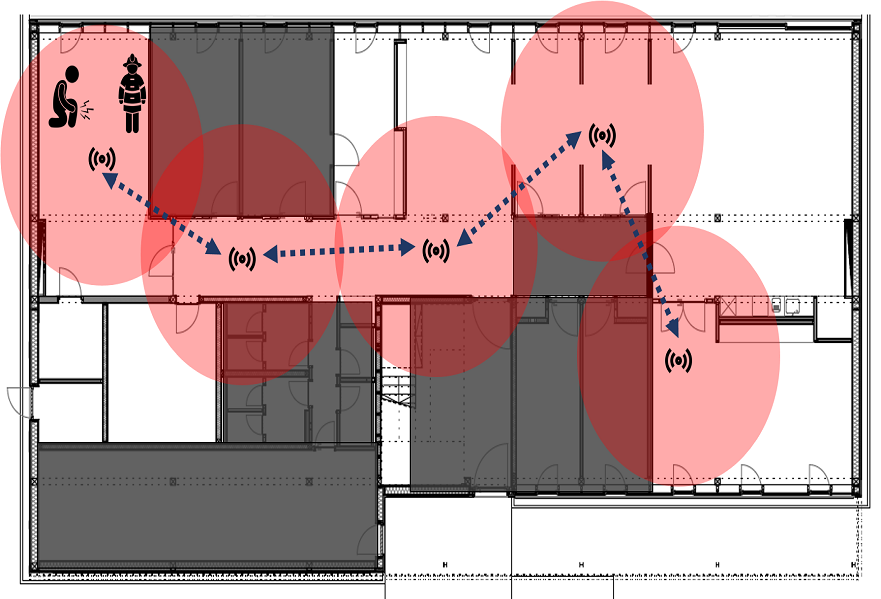
\includegraphics[scale=0.35]{Introduzione/intervento_step_5.png}
		\caption{Rete allo step 5 dell'esploratore}
		\label{fig:step5}
	\end{minipage}
	\ \hspace{10 mm} \
	\begin{minipage}[b]{6cm}
		\centering
		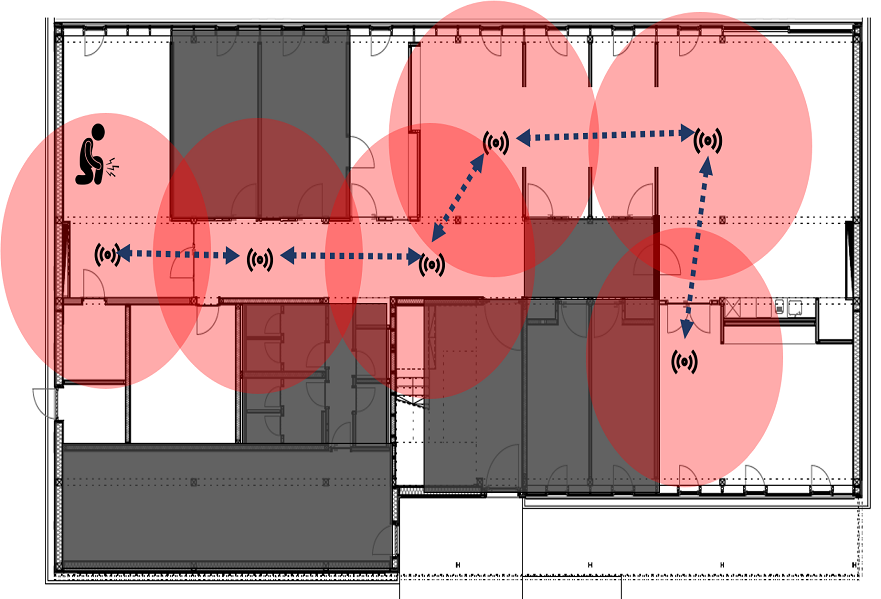
\includegraphics[scale=0.35]{Introduzione/intervento_step_6.png}
		\caption{Rete allo step 6 dell'esploratore}
		\label{fig:step6}
	\end{minipage}
\end{figure}
\newpage
Una volta creata l’infrastruttura, gli operatori potranno comunicare e condividere informazioni come posizione e stato. \newline
La presente tesi è così strutturata:
\begin{description}
\item [Capitolo 1:] Viene descritto il problema della geolocalizzazione indoor, il sistema ideato e le sue parti realizzate nel contesto di questa tesi.
\item [Capitolo 2:] Vengono illustrate le tecnologie utilizzate (sensori MEMS e UWB).
\item [Capitolo 3:] Viene descritto il rumore dei dati grezzi, le tecniche di raffinamento e alcuni algoritmi di data fusion.
\item [Capitolo 4:] Si riporta l'implementazione software e hardware del sottosistema realizzato.
\item [Capitolo 5:] Viene illustrato il procedimento di validazione e l'analisi dei dati ottenuti mediante algoritmi di data fusion.
\end{description}
\chapter{Contesto applicativo }
\label{contesto}
Nella parte iniziale di questo capitolo viene esplicato il contesto applicativo di questa tesi, una volta delineato vengono illustrate le tecniche basilari più utilizzate in questo ambito.

\section{Context-aware computing}
\label{context-aware}
Il sistema realizzato nell'ambito di questa tesi, si colloca nel paradigma di computazione noto come \textit{Context-aware computing}, ovvero un'applicazione nel quale i servizi utilizzano informazioni relative al contesto. In \cite{context} si definisce come \textit{context}:

\begin{quotation}
\textit{Ogni informazione che può essere usata per caratterizzare la situazione di un'entità. Ovvero una persona, un posto o un oggetto che è considerato rilevante all'interazione tra l'utente e l'applicazione, inclusi quest'ultimi.}
\end{quotation}

Questa definizione facilita il lavoro di progettazione e sviluppo di un applicazione permettendo di identificare quali informazioni sono importanti e quali no.
Si consideri un'applicazione nel quale l'utente deve registrare il peso degli oggetti presenti nel magazzino tramite una bilancia come mostrato dalla Fig.\ref{fig:context}:

\begin{figure}[H]  
	\centering 
	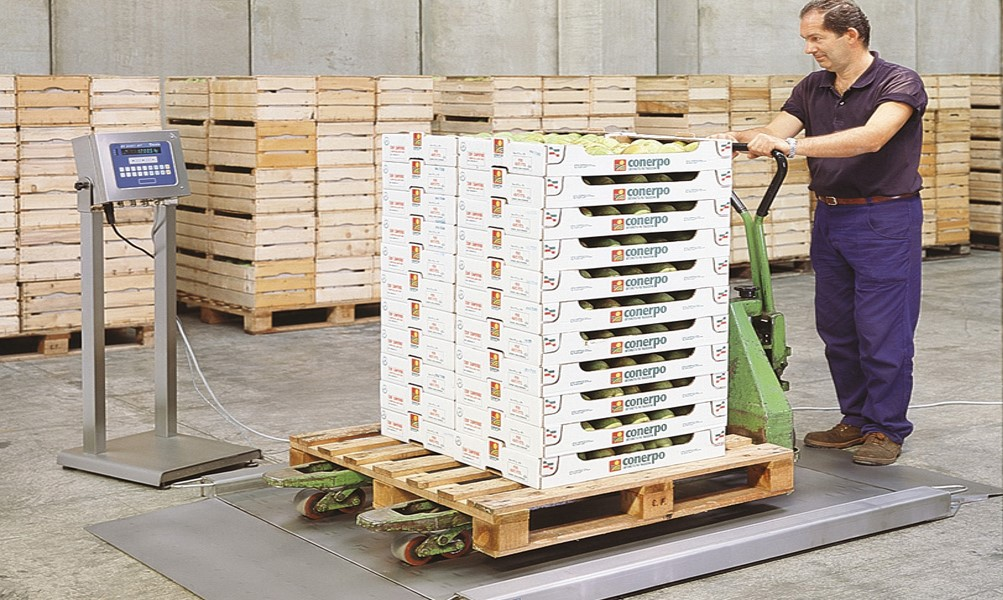
\includegraphics[scale=0.4 ]{ContestoApplicativo/bilancia.jpg}
	\caption{Esempio esplicativo del concetto di contesto}
	\label{fig:context}
\end{figure}
Nello scenario descritto le \textit{entità} sono rispettivamente utente e sistema, mentre due possibili informazioni riguardanti il contesto sono la presenza di altre persone e la posizione geografica del magazzino.\\
La presenza di altre persone nelle vicinanze non influisce il compito dell'utente, quindi non può essere considerato come informazione contestuale. La posizione geografica del magazzino invece si, infatti se quest'ultimo fosse situato in Italia il peso verrebbe calcolato in chilogrammi mentre se fosse situato negli USA verrebbe calcolato in libbre.\\
I sistemi che reperiscono, usano o interpretano queste informazioni contestuali sono detti \textit{context-aware} e vengono definiti in \cite{context} come:
\begin{quotation}
	\textit{Un sistema è context-aware se usa il contesto per fornire informazioni rilevanti e/o servizi agli utenti, dove la rilevanza dipende dal compito degli utenti.}
\end{quotation}
Uno dei tipi di context-aware più utilizzati si basa sul contesto della localizzazione, ovvero servizi basati sulla conoscenza di dove qualcosa o qualcuno si trovi. Nell'era moderna i servizi basati sulla localizzazione (in inglese: Location based services LBSs) stanno assumendo sempre più importanza nelle attività quotidiane dell'uomo grazie alle molteplici possibili applicazioni, tra le quali navigazione assistita per autoveicoli, tracking di persone sensibili (bambini, anziani, malati), servizi di emergenza e così via.\\
I LBSs vengono divisi in due macro categorie:
\begin{itemize}
	\item \textbf{OPSs}: Outdoor Positioning System Service, ovvero servizi di localizzazione in ambienti aperti.
	\item \textbf{IPSs}: Indoor Positioning System Service, ovvero servizi di localizzazione in ambienti indoor.
\end{itemize}
La tecnologia satellitare nota come Global Positioning System (GPS) è la tecnologia dominante negli OPSs. Attraverso una rete dedicata di satelliti artificiali in orbita, fornisce ad un terminale mobile o ricevitore GPS informazioni sulle sue coordinate geografiche ed orario, in ogni condizione meteorologica, ovunque sulla Terra o nelle sue immediate vicinanze ove vi sia un contatto privo di ostacoli con almeno quattro satelliti del sistema. La localizzazione avviene tramite la trasmissione di un segnale radio da parte di ciascun satellite e l'elaborazione dei segnali ricevuti da parte del ricevitore \cite{gps}.\\ 
Il grande limite di questa tecnologia è che i ricevitori devono essere nella line of sight (letteralmente a vista d'occhio) di almeno quattro satelliti nel cielo, questo significa che all'interno di edifici e spazi chiusi il segnale viene attenuato e i sistemi perdono di accuratezza. Quindi la tecnologia GPS non è adatta ai servizi di localizzazione indoor.\\
Il sistema realizzato nell'ambito di questa tesi si colloca nell'ambito degli IPSs approfonditi nel paragrafo successivo.


\section{Indoor Positioning System Service}
\label{IPS}
Un sistema di posizionamento indoor (in inglese: Indoor positioning system o IPS) è un sistema in grado di localizzare \textit{oggetti} o \textit{persone} all'interno di edifici utilizzando onde radio, campi magnetici, segnali acustici e/o altre informazioni raccolte dai sensori all'interno di dispositivi mobili \cite{IPS} o da altri  appositamente installati nell'ambiente. Questi sono una specializzazione dei più generici sistemi \textbf{RTLS}, standardizzati dall'\textit{International
Organization for Standardization and the International Electro Technical Commission} (ISO/IEC 24730). Lo standard definisce i sistemi RTLS come:
\begin{quotation}
	\textit{“ I Real time locating system sono sistemi wireless con l'abilità di localizzare la posizione di oggetti ovunque essi siano in uno spazio definito in un certo momento che è, o si avvicina, real time. La posizione è derivata dalla misurazione delle proprietà fisiche del collegamento radio."}
\end{quotation}
La differenza tra RTLS e IPS è che i primi sono stati pensati per le compagnie che vogliono tracciare i propri oggetti e le persone, fornendo uno storico di dove sono stati e dove si trovano ora, mentre gli IPS sono pensati per essere utilizzati da utenti su dispositivi mobili per navigare ed orientarsi all'interno di edifici.
Come già accennato, gli IPS \cite{IPS2} permettono di creare una vasta gamma di servizi, ad esempio:
\begin{itemize}
	\item\textbf{Way-Finding}: permettere di navigare in edifici complessi, come ad esempio aeroporti, seguendo il percorso indicato.
	\item\textbf{Ricerca dei punti d'interesse}, aumentare la customer experience facendo trovare all’utente ciò che desidera.
	\item \textbf{Multi-Dot}: visualizzare in una mappa le posizioni degli utenti per tracciare persone potenzialmente in pericolo (bambini, anziani).
	\item \textbf{Marketing di prossimità}: realizzare marketing mirati, inviando annunci sulle ultime offerte.
\end{itemize}
L’elenco di cui sopra rappresenta solo un ridotto sottoinsieme dei potenziali campi applicativi (vedi Fig.\ref{fig:surveyApplication}), per questo motivo negli ultimi anni \cite{indoorThesis} l'interesse nella ricerca e nello sviluppo di sistemi di questo tipo è cresciuto sempre più tra le aziende, che hanno percepito la possibilità di grandi profitti in un mercato non ancora esplorato del tutto.
\begin{figure}[H]  
	\centering 
	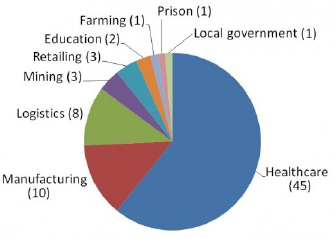
\includegraphics[scale=1.2]{ContestoApplicativo/application.png}
	\caption{Sondaggio tra 74 casi di studio di applicazioni IPS \cite{market}}
	\label{fig:surveyApplication}
\end{figure}

Secondo un sondaggio  di \textit{Markets and Markets} e un articolo pubblicato da\textit{ The International News Magazine}, il mercato degli IPS subirà una crescita annuale media del 42.1\% arrivando a valere 2.60 bilioni di dollari nel 2018. Questo da un'idea del perché grandi aziende come Google, Sony, Microsoft e Apple stiano investendo in questo settore.\\
Un'ulteriore spinta è data dal fatto che, al contrario del GPS per gli OPS (vedi \ref{context-aware}), tuttora non esiste uno standard di riferimento per gli IPS. Infatti sul mercato sono disponibili diversi tipi di IPS commerciali che si differenziano in base al principio di funzionamento e alle tecniche utilizzate, utilizzando hardware specifico o la combinazione di più sistemi.\\ 




\section{Stima della posizione}
\label{metodi_distanza}
Gli IPS possono essere classificati sulla base di diversi fattori, uno di questi è su come determinano la posizione dei.\\
Stimare \cite{IPS2} la distanza tra dispositivi wireless è utile perché attraverso questa informazione è possibile determinarne (con un certo errore) la posizione di un ricevitore rispetto ad un trasmettitore (\cite{alg1}, \cite{alg2}), queste tecniche si distinguono in:

	\begin{itemize}
	\item \textbf{Range based}:
	
		\begin{itemize}
		\item \textit{RSSI}- potenza del segnale radio ricevuto(sez.\ref{rssi})
		\item \textit{ToA} - tempo d’arrivo: (sez.\ref{toa})
		\item \textit{TDoA} - differenze del tempo di arrivo (sez.\ref{tdoa});
 	    \end{itemize}
     
	\item \textbf{Angle based}:
		\begin{itemize}
			\item \textit{AoA} - Angle of Arrival (sez.\ref{aoa}).
		\end{itemize}
		
\end{itemize}
Per poter determinare le distanze si devono distinguere i punti di riferimento (che hanno
delle coordinate note) dai nodi senza posizione nota a cui assegnare delle coordinate.
Si dicono:
\begin{itemize}
	\item \textbf{Anchor}: i nodi le cui coordinate sono note
	\item \textbf{Target}: il nodo di cui non si conosce la posizione.
\end{itemize}

 L’obiettivo del posizionamento è assegnare le giuste coordinate agli Unknown rispetto ad un sistema di riferimento. Questo è strettamente legato all'implementazione dell'IPS e così anche la codifica delle posizioni all'interno del sistema di riferimento, le coordinate potrebbero essere restituite all'utente in maniera relativa ("vicino alla cucina") oppure assoluta ("tre  metri in direzione ovest dal nodo 1").

\subsection{Range based}
Nel posizionamento dei nodi basato sulla distanza la stima della posizione del target dipende dai seguenti parametri:
	\begin{itemize}
	\item il tempo trascorso tra l’emissione e la ricezione del segnale radio;
	\item la distanza euclidea tra ogni emettitore ed il ricevitore;
	\item la potenza del segnale ricevuto.
\end{itemize}
In alcuni casi sono necessarie tre o più Anchor per ottenere le coordinate da assegnare allo Unknown.

\subsubsection{Received Signal Strength Indicator - RSSI}
\label{rssi}
La comunicazione \cite{IPS2} tra dispositivi wireless (senza fili) avviene tramite lo scambio di segnali propagati nell’aria. Durante la propagazione i segnali tendono ad attenuarsi con l'aumentare della distanza percorsa fino a non essere più percepibili.

\begin{figure}[H]  
	\centering 
	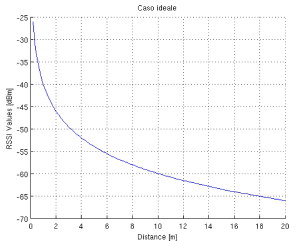
\includegraphics[scale=1.2]{ContestoApplicativo/signal.PNG}
	\caption{RSSI - Andamento della potenza in funzione della distanza percorsa dal segnale}
	\label{fig:signal}
\end{figure}

La stima della potenza del segnale ricevuto è data dall’indicatore RSSI \cite{rssi}. La distanza emettitore-ricevitore si stima utilizzando \textbf{l’equazione di trasmissione di Friis}.

\begin{equation}
		P_{T}=P_{R} \dfrac{G_{T}G_{R}\lambda^2}{(4\pi)^2d^n}
		\label{eq1}
\end{equation}

dove:
\begin{itemize}
	\item $P_{R}$: potenza del segnale ricevuto (Watt)
	\item $P_{T}$: potenza del segnale trasmesso(Watt)
	\item $G_{R}$: guadagno dell'antenna ricevente
	\item $G_{T}$: guadagno dell'antenna trasmittente
	\item $\lambda=\frac{v}{f}$: lunghezza d'onda, dove $v$ è la velocità di propagazione e $f$ è la frequenza dell'onda
	\item $d$: distanza espressa in metri
	\item $n$: constante di propagazione del segnale che dipende dall'ambiente 
\end{itemize}

Con la seguente equazione invece è possibile convertire la potenza espressa in Watt nella potenza espressa in dBm:
\begin{equation}
P[dBm] = 10\log_{10}(10^3P[W])
\label{eq2}
\end{equation}
Combinando l'equazione \ref{eq1} con \ref{eq2} e applicando le proprietà dei logaritmi si ottiene:
\begin{equation}
RSSI = -(10 n \log_{10} d - A)
\label{eq3}
\end{equation}
dove $A$ è la potenza del segnale ricevuto a distanza fissa di un metro (espressa in dBm), considerando una costante di propagazione $n$.\\
La stima della distanza si ottiene infine dalla seguente equazione:
\begin{equation}
d = 10 (\frac{A - RSSI}{10n})
\label{eq4}
\end{equation}
Tuttavia la distanza restituita non è del tutto precisa, infatti la potenza del segnale potrebbe essere alterata dall'ambiente circostante attraverso i fenomeni di \textbf{Riflessione} (il segnale sbatte e si riflette su vari ostacoli seguendo più percorsi) e di \textbf{Assorbimento} (il decadimento viene alterato dagli oggetti presenti). Tale tecnica viene solitamente completata utilizzando il metodo della \textbf{Trilaterazione} (sez.\ref{trilaterazione})\\


\subsubsection{Time Of Arrival measurements}  
\label{toa}
A differenza del precedente metodo, con questa tecnica la distanza tra emettitore e ricevitore viene stimata sulla base del tempo impiegato dal segnale a raggiungere il ricevitore. Nello specifico la sequenza di azioni è:
\begin{enumerate}
	\item Il nodo \textit{A} invia il segnale al tempo $t_1$
	\item Il segnale arriva al nodo \textit{B} al tempo $t_2$
	\item \textit{B} elabora il messaggio impiegando un tempo $t_d$ e lo invia al tempo $t_3$
	\item Il segnale torna al nodo \textit{A} al tempo $t_4$
\end{enumerate}
Come mostrato dalla figura seguente:

\begin{figure}[H]  
	\centering 
	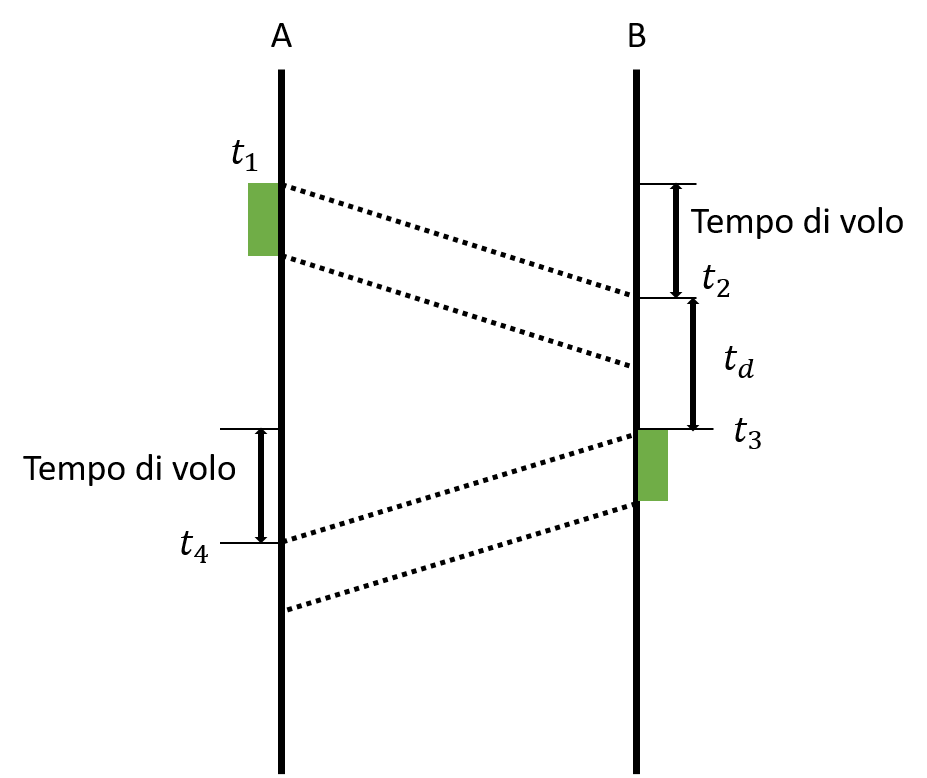
\includegraphics[scale=0.4]{ContestoApplicativo/toa.png}
	\caption{ToA - Principio di funzionamento}
	\label{fig:toa}
\end{figure}

Quindi il tempo di viaggio può essere ricavato con la seguente equazione:

\begin{equation}
t_d = \dfrac{(t_4 - t_1) - (t_3 - t_2)}{2}
\label{td}
\end{equation}

E infine la distanza stimata attraverso:
\begin{equation}
d_{ToA} = t_d * c
\label{eq:toa}
\end{equation}

dove $c$ è la velocità di propagazione della luce nel vuoto pari a 299792458 m/s. Per identificare in modo univoco un target, questa tecnica viene completata dalla tecnica di posizionamento nota come \textbf{Trilaterazione} (sez. \ref{trilaterazione}), come per le misure RSSI viste precedentemente.\\
Il difetto principale di questa tecnica consiste nel fatto che sistemi utilizzati devono avere un complesso meccanismo di sincronizzazione per mantenere una fonte affidabile di tempo per i sensori\cite{toaProblem}.

\subsubsection{Time Difference Of Arrival}
\label{tdoa}
Questa tecnica è basata sulla differenza nel tempo di arrivo di un segnale emesso da due sorgenti diverse verso un altro nodo, come mostrato in Fig.\ref{fig:tdoa}).

\begin{figure}[H]  
	\centering 
	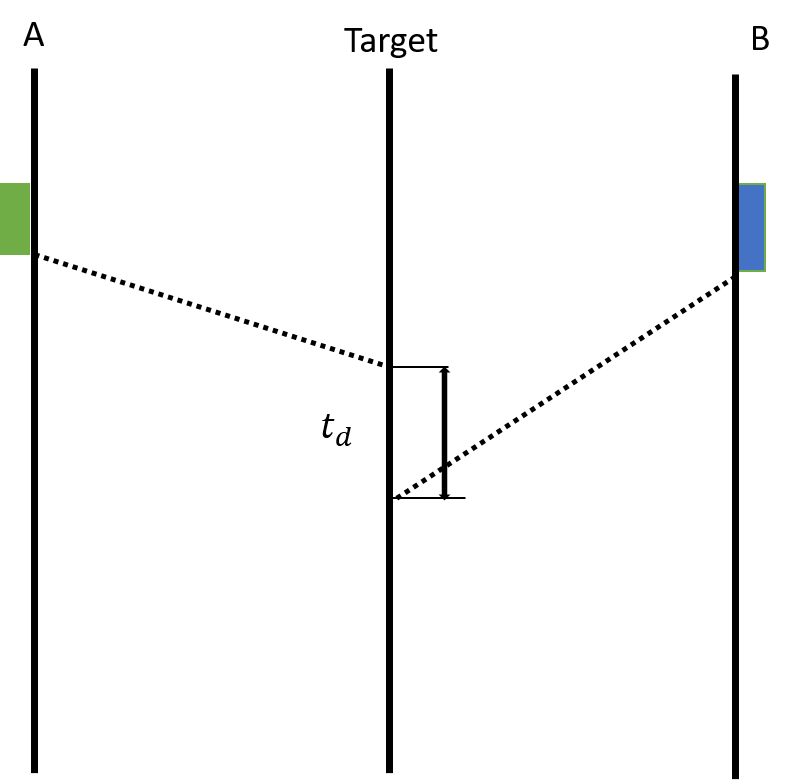
\includegraphics[scale=0.4]{ContestoApplicativo/tdoa.png}
	\caption{TDoA - Principio di funzionamento}
	\label{fig:tdoa}
\end{figure}
Se si suppongono note le posizioni dei nodi \textit{A} e \textit{B} rispetto ad un sistema di riferimento, indicate rispettivamente dalle tuple $(x_B,y_B)$ e $(x_A,y_A)$, la distanza del nodo \textit{Target} può essere stimata dalla seguente equazione:
 
\begin{equation}
\Delta d = \Delta t_d * c
\label{eq:tdoa}
\end{equation}

Dove:
\begin{itemize}
	\item $c$ è la velocità di propagazione della luce nel vuoto
	\item $ \Delta t$ è la differenza del tempo di arrivo dei segnali emessi dai nodi \textit{A} e \textit{B}
	\item $\Delta d$ è la distanza in due dimensioni: $(\sqrt{(x_B-x)^2 + (y_B-y)^2}- \sqrt{(x_A-x)^2 + (y_A-y)^2})$ 
\end{itemize}

In questo modo, la posizione del \textit{target} viene stimata all'interno del luogo geometrico dei punti del piano aventi come costante la differenza delle distanze tra i nodi, ovvero dall'iperbole avente come fuochi i nodi \textit{A} e \textit{B}. Come mostrato in Fig.

\begin{figure}[H]  
	\centering 
	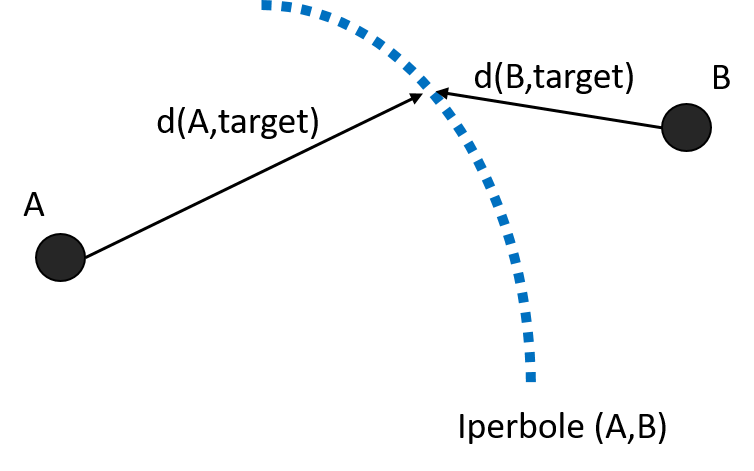
\includegraphics[scale=0.4]{ContestoApplicativo/tdoa1.png}
	\caption{TDoA - Stima della posizione lungo l'iperbole identificata da due nodi}
	\label{fig:tdoa1}
\end{figure}

	Tuttavia così facendo la posizione del \textit{target} rimane stimata in un'insieme di punti infinito, quindi come per le tecniche viste precedentemente (\ref{rssi} e \ref{toa}) per identificare in modo univoco il target questa tecnica ha bisogno di essere completata dalla tecnica di posizionamento nota come \textbf{Trilaterazione} \ref{trilaterazione}.

\subsection{Angle Based}
\label{angle}
\subsubsection{Angle of Arrival}
\label{aoa}
Con questa tecnica la posizione del \textit{target} viene stimata misurando gli angoli di incidenza del segnale trasmesso ad altri nodi.\\
Si consideri \cite{aoa} un antenna in un canale di propagazione, la tensione del segnale ricevuto (\ref{fig:aoa}) è data dalla seguente equazione:\\
\begin{equation}
 V = \int_{0}^{2\pi} AoA(\varphi) G(\varphi)d\varphi 
\end{equation}

Dove:
\begin{itemize}
	\item $AoA(\varphi)$ rappresenta l'ampiezza e la fase dell'onda incidente
	\item $G(\varphi)$ è il campo elettrico del nodo target 
	\item $C$ valore proporzionale constante
\end{itemize}

Se si ruota l'antenna di un angolo $\alpha$ intorno a se stessa nel piano cartesiano la precedente equazione diventa:
\begin{equation}
\label{eq:2}
V (\alpha) = \int_{0}^{2\pi} AoA(\alpha-\varphi) G(\varphi)d\varphi 
\end{equation}

Possiamo notare che l'Eq.\ref{eq:2} è la convoluzione di $AoA$ e $G$ e può essere scritta nel seguente modo:
\begin{equation}
\label{eq:3}
V (\alpha) = C AoA(\alpha) * G(\alpha)
\end{equation}

Si è scelto di normalizzare l'Eq.\ref{eq:3} con il valore constante $C$. Quindi, utilizzando la transformata di Fourier l'Eq.\ref{eq:3} diventa:

\begin{equation}
\label{eq:4}
F(V(\alpha)) = F(AoA(\alpha)) F(G(\alpha))
\end{equation}

Da cui è possibile calcolare l'angolo di incidenza desiderato:

\begin{equation}
\label{eq:5}
AoA(\alpha) = F^{-1} \dfrac{F(V(\alpha))}{F(G(\alpha))} \quad se \quad F(G(\alpha))\neq 0
\end{equation}

\begin{figure}[H]  
	\centering 
	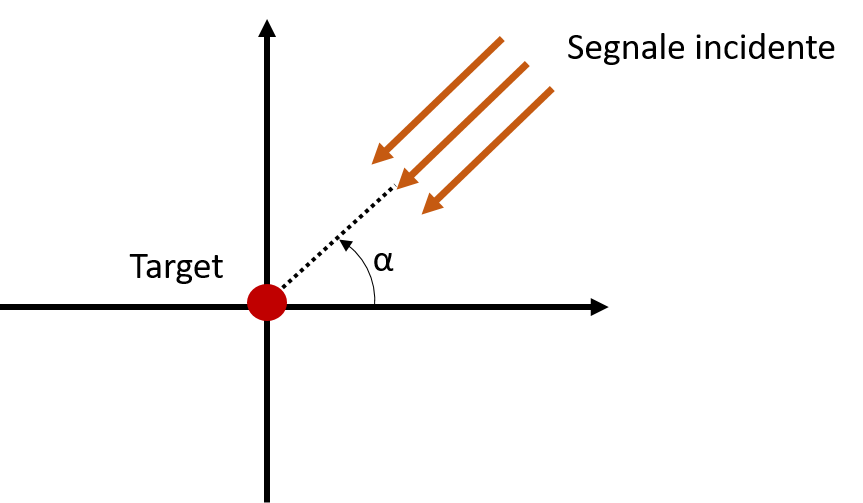
\includegraphics[scale=0.4]{ContestoApplicativo/aoa.png}
	\caption{AoA - Stima della posizione attraverso l'angolo di incidenza}
	\label{fig:aoa}
\end{figure}

Il vantaggio dell’AoA risiede nella possibilità di ottenere un risultato attendibile senza la necessità di informazioni riguardanti i tempi di trasmissione. A fronte del risparmio dal punto di vista computazionale, la tecnica presenta alcuni svantaggi pratici, dovuti al costo dell’hardware, che al fine di restituire informazioni precise, deve essere di alta qualità; rischiando altrimenti di incorrere in fenomeni che comprometterebbero la misurazione. Per questo motivo solitamente questa tecnica viene completata dalla tecnica di posizionamento nota come \textit{Triangolazione} (\ref{triangolazione}).


\section{Tecniche di localizzazione}
Per tecniche di localizzazione si intendono tutte quelle tecniche che, combinate alle differenti metodologie di stima della posizione viste precedentemente (vedi \ref{metodi_distanza}), permettono di localizzare un nodo \textit{target} all'interno di un sistema di riferimento.\\
In questo paragrafo vengono illustrate quelle più conosciute e basilari nell'ambito degli IPS.

\subsection{MIN-MAX}
Combina le stime della distanza di più \textit{anchor}, ottenute attraverso tecnica \textit{RSSI} (\ref{rssi}), nel seguente modo:

\begin{itemize}
	\item Stimare la distanza $d_i$ di ogni nodo i-esimo in base al valore RSSI
	\item Traccia due linee orizzontali e verticali a distanza $d_i$ dallo nodo \textit{target}
	\item Identifica un quadrato di lato 2  $d_i$ i cui estremi saranno: \\
			$[max(x_i-d:i),max(y_i-d_i)] * [min(x_i+d_i),min(y_i+d_i))]$
	\item Calcola le intersezioni dei quadrati
\end{itemize}

Il centro del quadrato (Fig.\ref{fig:minmax}) rappresenta la posizione stimata del \textit{target}. Più piccola sarà l’area e maggiore sarà l’accuratezza della posizione stimata.
\begin{figure}[H]  
	\centering 
	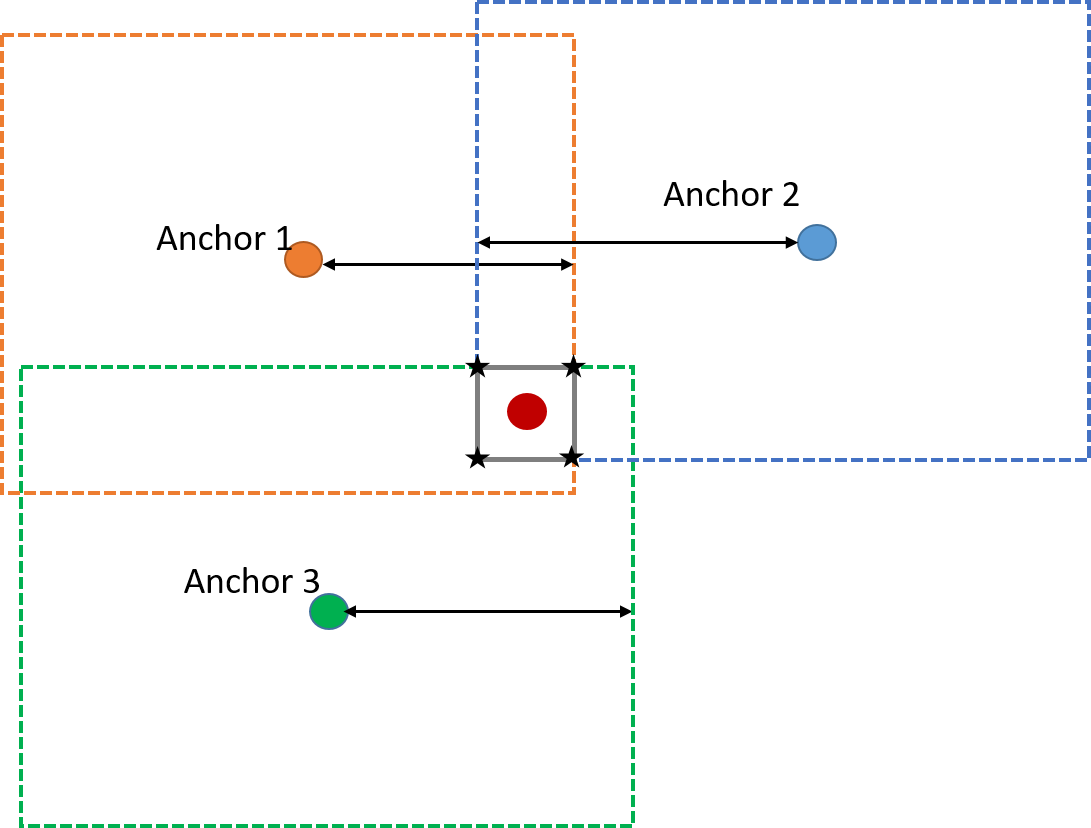
\includegraphics[scale=0.4]{ContestoApplicativo/minmax.png}
	\caption{MIN-MAX - Tecnica di posizionamento }
	\label{fig:minmax}
\end{figure}



\subsection{Trilaterazione}
\label{trilaterazione}
Consideriamo 3 \textit{Anchor} intorno cui disegniamo 3 circonferenze aventi per centro le coordinate degli \textit{Anchor} e per raggio l'RSSI del segnale ricevuto dallo \textit{Uknown}, come mostrato in figura:
\begin{figure}[H]  
	\centering 
	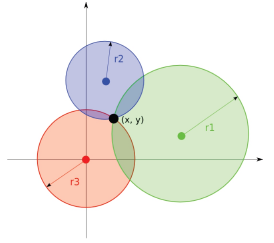
\includegraphics[scale=0.8]{ContestoApplicativo/trilaterazione.png}
	\caption{Trilaterazione - Esempio esplicativo}
	\label{fig:trilaterazione}
\end{figure}
Quindi le coordinate dell'Unknown sono la soluzione del seguente sistema:
\begin{equation}
\begin{cases}
(x-x_1)^2 + (y-y_1)^2 = r_1^2\\
(x-x_2)^2 + (y-y_2)^2 = r_2^2\\
(x-x_3)^2 + (y-y_3)^2 = r_3^2
\end{cases}
\end{equation}
In base alla soluzione del sistema si può avere una delle seguenti situazioni:
\begin{itemize}
	\item La soluzione non è unica, si hanno tre cerchi che si sovrappongono
	\item Il sistema non ammette soluzione, i raggi vanno aumentati
	\item La soluzione esiste ed è unica, i tre cerchi si intersecano in un solo punto
\end{itemize}



\subsection{Triangolazione}
\label{triangolazione}
A differenza delle Trilaterazione (\ref{trilaterazione}), queste tecniche identificano la posizione del nodo \textit{target} a partire dagli angoli stimati da tre anchors attraverso una delle teniche Angle Based (\ref{angle}).\\
In \cite{triangolazione} si descrive la triangolazione geometrica attraverso il seguente algoritmo:\\

\begin{enumerate}
   \item Siano \textit{1,2 e 3} le anchor in grado di stimare l'angolo, rispetto ad una circonferenza concentrica all'anchor stessa, del nodo target
   \item siano $L_{12}$ e $L_{31}$ rispettivamente le distanze tra l'anchor 1 e 2 e l'anchor 3 e 1
   \item Siano gli angoli compresi tra \textit{1} e \textit{2} e tra \textit{1} e \textit{3}, indicati rispettivamente con $\lambda_{12} e \lambda_{13}$, minori di 180°
   \item sia $\phi$ l'angolo tra l'asse x positivo e la linea formata dall'anchor \textit{1} e \textit{2}
   \item sia $\sigma$ l'angoolo tra l'asse x positivo, l'anchor \textit{1} e l'anchor \textit{3} più $\phi$
   \item sia $\gamma= \sigma - \lambda_{31}$
   \item sia $p= \dfrac{L_{31} \sin\lambda_{12}}{L_{12} \sin\lambda_{31}}$
   \item sia $\tau= \tan^{-1} \dfrac{\sin\lambda{12}-p \sin\gamma}{p \cos\gamma-\cos\lambda{12}}$
   \item sia $L_1 = \dfrac{L_{12} sin(\tau+\lambda_{12})}{\sin\lambda_{12}}$
\end{enumerate}

Allora le coordinate $x$ e $y$ del target sono date da:
\begin{itemize}
	\item $x_R = x_1 - L_1  \cos(\phi + \tau)$
	\item $y_R = y_1 - L_1  \sin(\phi + \tau)$
	\item $\Phi_R = \phi + \tau - \lambda_1$
\end{itemize}
Dove $\Phi_R$ rappresenta l'orientamento del nodo target, come mostrato in Fig.\ref{fig:triangolazione}.


\begin{figure}[H]  
	\centering 
	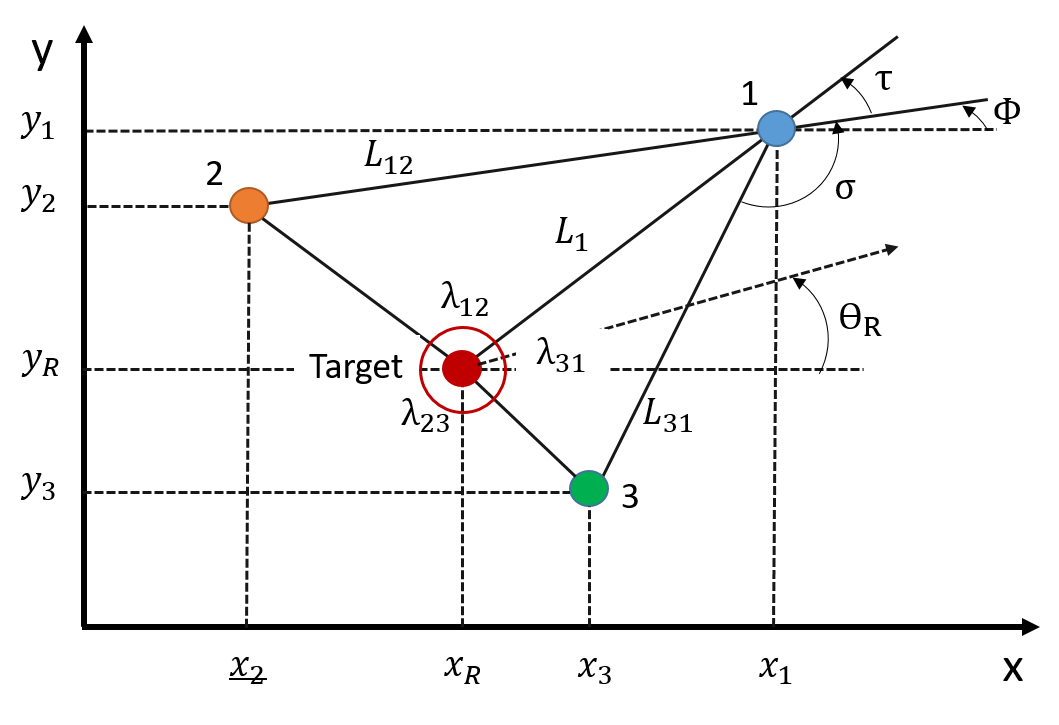
\includegraphics[scale=0.4]{ContestoApplicativo/triangolazione.png}
	\caption{Triangolazione - Esempio esplicativo}
	\label{fig:triangolazione}
\end{figure}





\section{Sensor Data Fusion}

In generale con Sensor Data Fusion si indicano tutte quelle tecniche che \cite{sensorfusion} combinano dati provenienti da sensori o derivate da altre risorse tali che l'informazione risultante ha una minore incertezza rispetto a quella ottenuta utilizzando le risorse individualmente. \\
Nel contesto degli IPS (\ref{IPS}), il Sensor Fusion ha come scopo quello di determinare informazioni riguardanti la posizione di oggetti e/o persone. Le risorse delle informazioni grezze sono le più svariate, tra le quali:
\begin{itemize}
	\item Accelerometro
	\item Giroscopio
	\item Magnetometro
	\item Infrarossi
	\item RFID 
	\item Sensori ottici
	\item Sensori di pressione
	\item Bluetooth
	\item WiFi
	\item Telecamera
	\item UWB
\end{itemize}

Come e quali risorse utilizzare per stimare la posizione di un oggetto è una sfida ingegneristica non banale, ma grazie alla crescente richiesta di IPSs la ricerca di nuove tecnologie e algoritmi in questo settore ha permesso di raggiungere risultati incredibili fino a qualche anno. \\








\chapter{Descrizione del sistema}
\label{scenario}
In questo capitolo si illustra inizialmente il macrosistema inerente al progetto aziendale, con tutti i suoi sottosistemi e i loro rispettivi obiettivi. Nel paragrafo successivo invece, viene approfondito il sottosistema realizzato specificandone i requisiti funzionali e non. 


\section{Il macrosistema}



\section{Il sistema realizzato}
\chapter{Unità di misura inerziale}
\label{tecnologie}
Le unità di misura inerziale \cite{mems} (in inglese Inertial Measurement Units - IMU) sono dispositivi elettronici basati su sensori inerziali come accelerometri (\ref{accell}) e giroscopi (\ref{giroscopi}). In molti casi a questi vengono aggiunti altri sensori utili ad applicazioni di navigazione come il magnetometro (\ref{magnetometro}). Nello specifico di questa tesi, l'IMU utilizzata è un circuito integrato composto da questi tre sensori (più altri non utilizzati come sensore di temperatura) realizzati tramite tecnologia MEMS (acronimo di Microelectro Mechanical System, ovvero sistemi meccanici microelettrici).\\
Nel corso degli anni l'interesse per questa tecnologia è cresciuto grazie ai vantaggi in termini economici e tecnici, tra questi i più importanti sono:
\begin{itemize}
	\item costo di realizzazione costante e proporzionale alla superficie del dispositivo
	\item grande potenziale di integrazione nei circuiti elettronici integrati
	\item basso consumo energetico
	\item dimensioni ridotte
\end{itemize}
 
 In questo capitolo si illustrano i principi di funzionamento alla base dei sensori, realizzati mediante tecnologia MEMS, integrati nell'IMU utilizzata nel lavoro di questa tesi.



\section{Accelerometro}
\label{accell}
In generale un accelerometro è un dispositivo in grado di misurare l’accelerazione di un corpo rigido causata da una forza esterna. Questa può essere statica, come la forza di gravità, o dinamica nel caso di forze vibranti applicate al dispositivo.\\
Uno dei più comuni accelerometri MEMS è quello \textit{capacitivo} che, come il nome suggerisce, si basa sulla \textit{capacità} elettrostatica. Se due piastre sono posizionate parallelamente tra di loro e poste ad una certa distanza, allora la capacità generata è data da:

\begin{equation}
\label{capacita}
C = \varepsilon_r \varepsilon_0 \dfrac{A}{d} 
\end{equation}
Dove:
\begin{itemize}
	\item $C$ è la capacità
	\item $\varepsilon_0$ è la constante dielettrica del vuoto
	\item $\varepsilon_r$ è la constante dielettrica relativa al materiale utilizzato per le piastre
	\item $A$ è l'area delle piastre
	\item $d$ è la distanza tra le due piastre
\end{itemize}
Dall'Eq.\ref{capacita} si noti che la capacità può variare solo se vi sono cambiamenti nell'area delle piastre o nella loro distanza. Proprio su quest'ultimo parametro si basano gli accelerometri capacitivi. Una classica struttura è rappresentata dalla Fig.\ref{fig:acc1}:
 \begin{figure}[H]  
	\centering 
	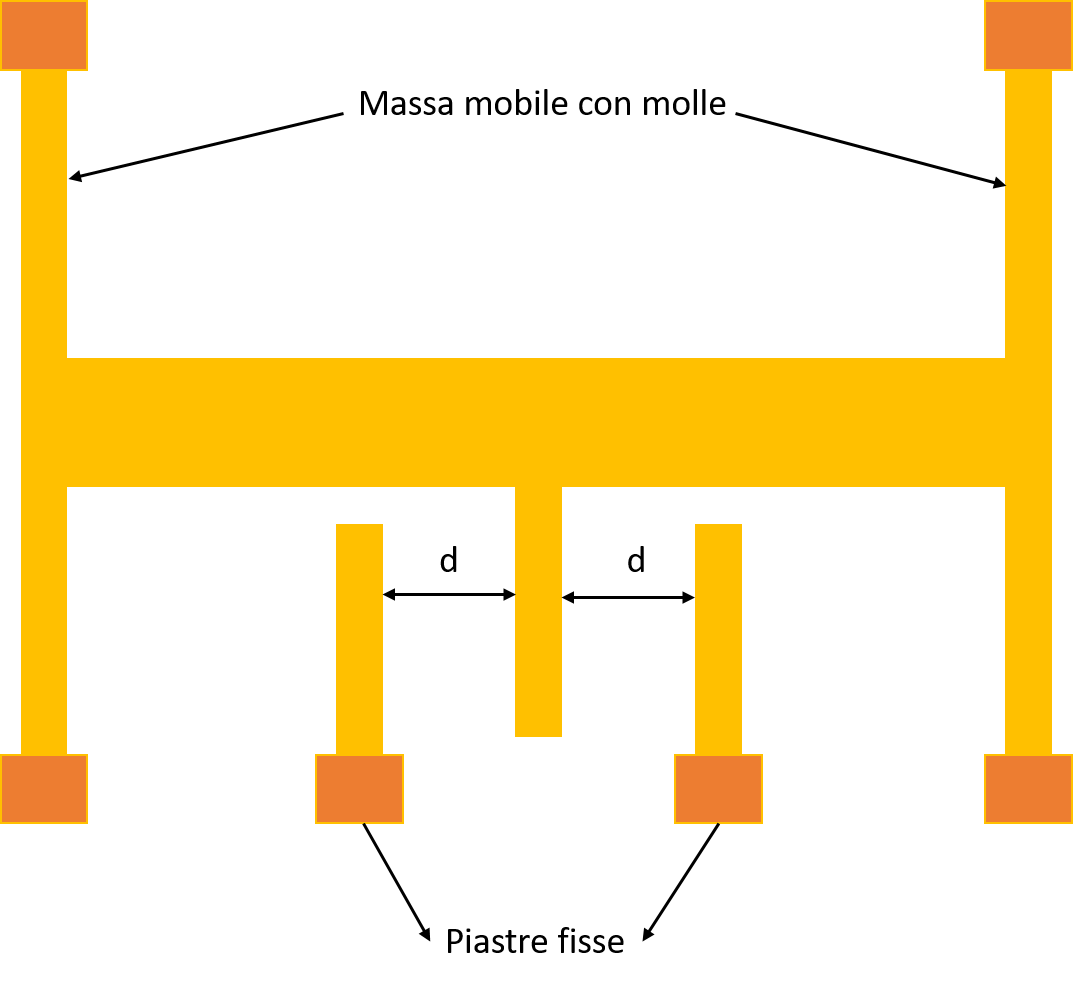
\includegraphics[scale=0.25 ]{tecnologie/acc1.png}
	\caption{Rappresentazione esemplificativa di un accelerometro capacitivo a riposo}
	\label{fig:acc1}
\end{figure}
La massa centrale è in grado di muoversi lungo un asse orizzontale grazie a delle molle poste alle sue estremità, come rappresentato in Fig.\ref{fig:acc2}:
 \begin{figure}[H]  
	\centering 
	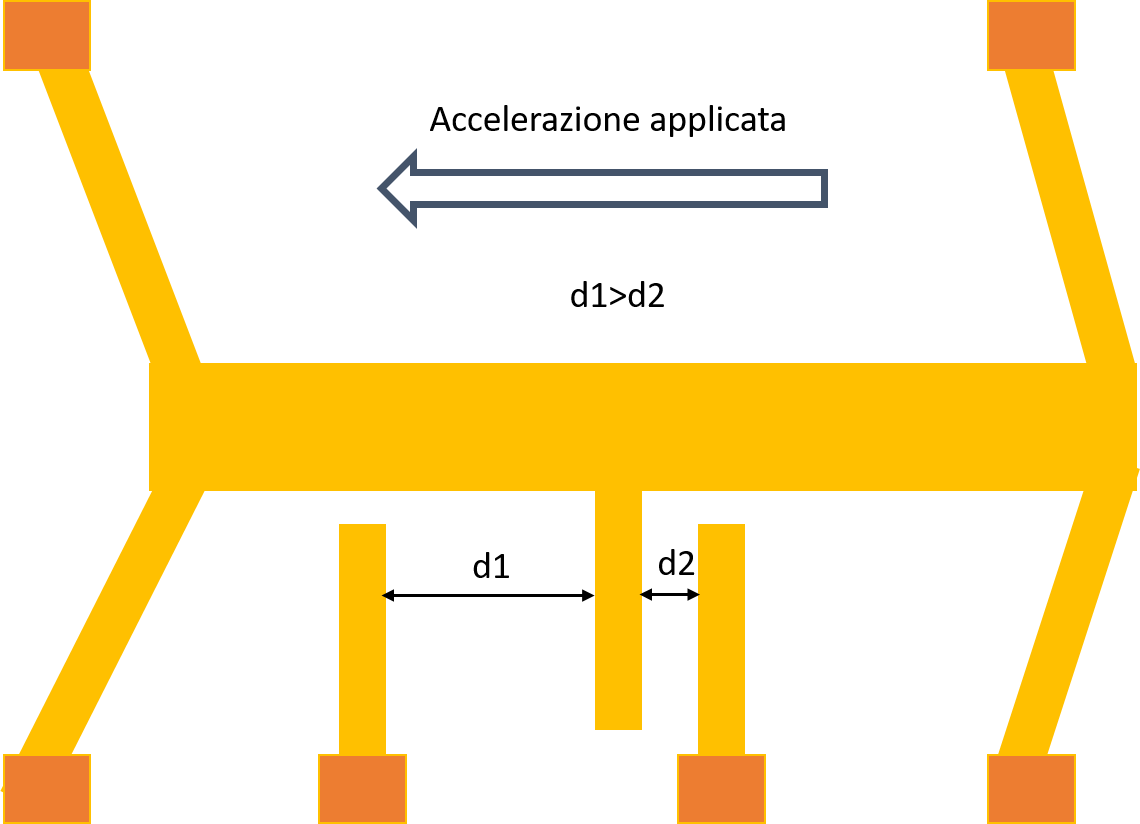
\includegraphics[scale=0.25 ]{tecnologie/acc2.png}
	\caption{Rappresentazione esemplificativa di un accelerometro capacitivo che subisce una forza esterna}
	\label{fig:acc2}
\end{figure}

A seguito del movimento della massa centrale, la distanza $d2$ in Fig.\ref{fig:acc2} si farà più piccola provocando una variazione di tensione ai capi della massa centrale. Questa verrà quindi convertita in un valore numerico rappresentante l'accelerazione subita in base alla scala e alla sensibilità del dispositivo.\\ 

\section{Giroscopio}
\label{giroscopi}
In generale, un giroscopio è un dispositivo in grado di misurare la velocità angolare a cui è sottoposto il dispositivo. I giroscopi realizzati mediante tecnologia MEMS si basano sulla forza di \textit{Coriolis}. In fisica \cite{corolois}, la forza di Coriolis è una forza apparente a cui risulta soggetto un corpo quando si osserva il suo moto da un sistema di riferimento che sia in moto circolare rispetto ad un sistema di riferimento inerziale. \\
I giroscopi di questo tipo sono composti \cite{gyroMems} da una \textit{massa} \textbf{m}, due \textit{molle} e due ammortizzatori come mostrato in Fig.\ref{fig:gyro}. Si assuma  l'asse x come l'asse di direzione (drive mode) e l'asse y come l'asse di rilevamento(sensing mode). Quando la massa è sottoposta ad una vibrazione armonica applicata da una forza elettrostatica, elettromagnetica o elettrotermica, lo spostamento lungo l'asse x è dato da:
\begin{equation}
x(t) = A_x \cos(\omega_x t)
\end{equation}
Dove $A_x$ è l'ampiezza e $\omega_x$ è la frequenza angolare.  Una velocità angolare $\Omega_z$ in input intorno all'asse z causa un'accelerazione di Coriolis lungo l'asse y data dalla seguente equazione:
\begin{equation}
a_y= 2\Omega_z \times \frac{d_x}{d_t}= -2\Omega_z A_x \omega_x \sin(\omega_x t)
\end{equation}

La massa quindi inizierà a vibrare lungo l'asse y a causa della forza di Coriolis e la velocità angolare $\Omega_z$ può essere calcolata misurando lo spostamento lungo l'asse vibrante. \\
Quando il \textit{drive mode} e il \textit{sense mode} sono perfettamente uguali ($\omega_x = \omega_y$), l'ampiezza lungo l'asse y raggiunge il massimo mentre la larghezza di banda raggiunge il minimo. In generale, questi due parametri dovrebbero essere uguali al fine di ottimizzare la sensibilità e la larghezza di banda.
 \begin{figure}[H]  
	\centering 
	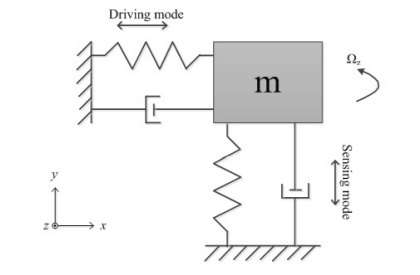
\includegraphics[scale=1]{tecnologie/gyro.png}
	\caption{Rappresentazione di un giroscopio vibrante per la misura della velocità angolare lungo l'asse z}
	\label{fig:gyro}
\end{figure}




\section{Magnetometro}
\label{magnetometro}
In generale, un magnetometro è un dispositivo in grado di rilevare l'intensità e la direzione del campo magnetico presente. Questi si basano sulla ben nota forza di Lorentz.\\
Se si eroga una certa corrente in un conduttore posto in un campo magnetico trasversale al flusso, si genera una forza proporzionale alla velocità dei portatori, alla carica ed al valore del campo magnetico, diretta nella direzione ortogonale ad entrambi, secondo la  relazione:
\begin{equation}
\overrightarrow{F_L} = q \overrightarrow{v} \times \overrightarrow{B}
\end{equation}
Dove:
\begin{itemize}
	\item $q$ è la carica elementare
	\item $F$ è la forza di Lorentz
	\item $B$ è il campo magnetico nel vuoto
\end{itemize}
Indicando con $l$ la lunghezza del conduttore si ha:
\begin{equation}
\overrightarrow{F_L} = l \overrightarrow{i} \times \overrightarrow{B}
\end{equation}
Questa forza viene quindi sfruttata per misurare il campo magnetico esterno agente sul dispositivo. Una delle realizzazioni più comuni nell'ambito dei sensori realizzati mediante tecnologia MEMS sono i magnetometri capacitivi.\\
In Fig.\ref{fig:magnet} è mostrata una semplice implementazione di un magnetometro capacitivo. Questo è composto da due \textit{molle} i cui terminali sono ancorati al substrato del dispositivo dove viene fatta circolare una corrente elettrica. Nel punto centrale le molle mantengono sospeso un \textit{rotore} dove idealmente non scorre corrente e al cui interno sono ancorati degli \textit{statori}. In presenza di una forza di Lorentz, le \textit{molle} si deformano dando origine ad uno spostamento rigido del \textit{rotore}. Poiché lo \textit{statore} non si muove, la capacità tra il \textit{rotore} e lo \textit{statore} cambia in maniera proporzionale all'intensità del campo magnetico esterno.
 \begin{figure}[H]  
	\centering 
	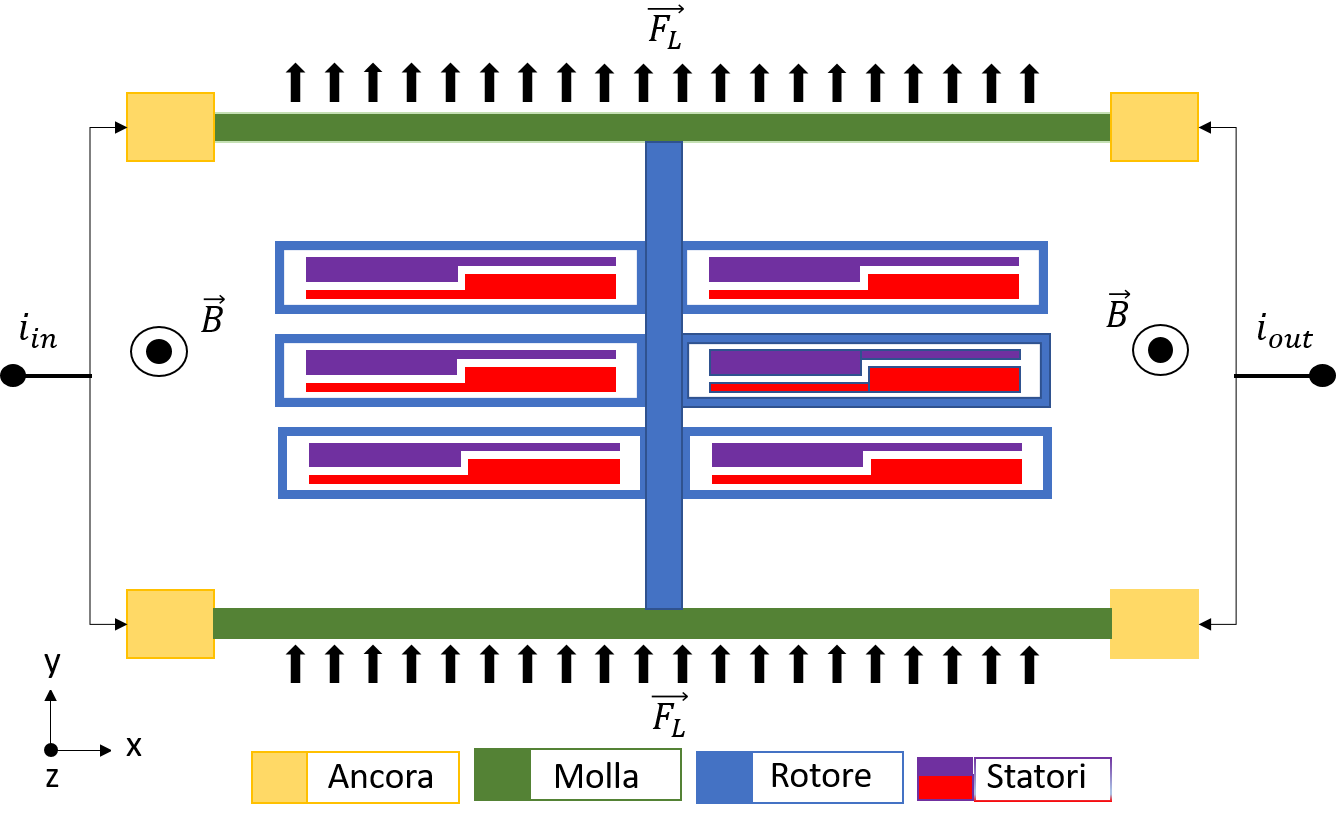
\includegraphics[scale=0.4 ]{tecnologie/magnet.png}
	\caption{Rappresentazione esemplificativa di un magnetometro capacitivo lungo l'asse \textit{z}}
	\label{fig:magnet}
\end{figure}


\section{Modello di misura}
\label{modello_di_misura}
Dopo aver introdotto i principi di funzionamento dei sensori è bene specificare il modello di misurazione.\\
I sensori utilizzati hanno tre assi lungo i quali una \textit{"quantità fisica"} (esempio forza, velocità angolare, campo magnetico) è convertita in un segnale di tensione in uscita. \\
Tipicamente questi sensori hanno un comportamento lineare nell'area di lavoro. Sulla base di questa osservazione, la seguente equazione (semplificata) descrive la relazione tra la forza fisica $y(t)$ e la tensione in uscita dal sensore $ u(t)$:

\begin{equation}
    u(t) = G R y(t) + c
\end{equation}
Dove:
\begin{itemize}
	\item $G$ è la matrice diagonale contenente il guadagno per ogni asse sensibile
	\item $R$ è la matrice di allineamento che specifica la direzione degli assi
	\item $c$ è il vettore di offset 
\end{itemize}
Al fine di discutere il modello di misura, si devono introdurre i seguenti sistemi di coordinate (in inglese: coordinate frames) rappresentati in Fig.\ref{fig:frames}:

\begin{itemize}
	\item Il \textbf{frame del corpo} - \textit{b-frame} (in inglese: \textit{body frame}): è il sistema							 di riferimento dei movimenti dell'IMU. L'origine è posta al centro dei sensori e allineata al case posto sul chip. Tutte le misure inerziali sono calcolate su questo sistema di riferimento.
	\item Il \textbf{frame di navigazione} - \textit{n-frame} (in inglese: \textit{navigation frame}) è il frame geografico nel quale vogliamo navigare. Per navigazioni a corto raggio è considerato statico rispetto alla terra.
	\item Il \textbf{frame inerziale} - \textit{i-frame} (in inglese: \textit{inertial frame}): è un frame stazionario non rotante. L'IMU misura le forze relativamente a questo frame. La sua origine è posta al centro della terra e i suoi assi sono allineati rispetto alle stelle.
	\item Il \textbf{frame terrestre} - \textit{e-frame} (in inglese: \textit{earth frame}): coincide con l' i-frame ma ruota intorno alla terra. L'origine è posta al centro della terra e gli assi fissati rispetto ad essa.
\end{itemize}



\begin{figure}[H]
	\centering    
	\label{fig:frames}
	\subfigure[]{\label{fig:framesa}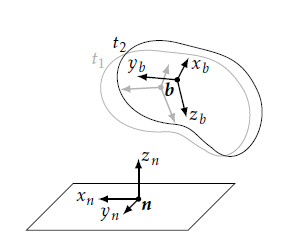
\includegraphics[width=60mm]{tecnologie/framesa.png}}
	\subfigure[]{\label{fig:framesb}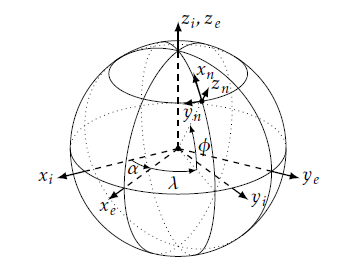
\includegraphics[width=60mm]{tecnologie/framesb.png}}
	\caption{in \ref{fig:framesa} il \textit{b-frame} nell'istante $t_1$ e $t_2$ relativamente al \textit{n-frame}, in \ref{fig:framesb} l'\textit{n-frame} in latitudine $\varphi$ e longitudine $\lambda$, l'\textit{e-frame} all'angolo $\alpha(t)= \omega_{ie}t$ e l'\textit{i-frame}}
\end{figure}
Ignorando la dipendenza dal tempo delle quantità coinvolte, la misura del giroscopio (si veda \ref{giroscopi}) è modellata in \cite{gyromodel} come:

\begin{equation}
y_\omega = \omega_{ib}^b + \delta_{\omega}^b + e_\omega^b
\end{equation}

Dove:
\begin{itemize}
	\item $\omega_{ib}$ è la velocità angolare nel \textit{b-frame} osservata dall'\textit{i-frame}
	\item $\delta_\omega$ è la deriva del sensore che varia lentamente nel tempo 
	\item $e_w^b$ è il rumore gaussiano
\end{itemize}

La velocità angolare $\omega_{ib}$ può essere così estesa:

\begin{equation}
\omega_{ib} = R^{bn} ( \omega_{ie}^n + \omega_{en}^n) + \omega_{nb}^b
\end{equation}

Dove:
\begin{itemize}
	\item $ R$ è la matrice di rotazione
	\item $\omega_{ie}$ è la velocità angolare della terra
	\item $\omega_{en}$ è velocità angolare di transporto
	\item $\omega_{nb}$ è la velocità angolare richiesta ai fini della navigazione
\end{itemize}

La misura dell'accelerometro $y_a$ è invece modellata in \cite{gyromodel} come:

\begin{equation}
\label{accelModel}
 y_a = f^b + \delta_a^b + e_a^b = R^{bn} (\ddot{b}_{ii}^n - g^n) + \delta_a^b + e_a^b
\end{equation}
Dove:
\begin{itemize}
	\item $f$ è la specifica forza esterna
	\item $\delta_a$ è la deriva del sensore che varia lentamente nel tempo 
	\item $e_a$ è il rumore gaussiano
\end{itemize}
L'Eq.\ref{accelModel} divide la forza specifica nei suoi contributi provenienti dall'accelerazione lineare del corpo osservata dall'\textit{i-frame} ($\ddot{b}_{ii}$) e dal vettore gravitazione $g$. L'accelerazione lineare può a sua volta essere espansa come:

\begin{equation}
\ddot{b}_{ii} = \omega_{ie}^n \times \omega_{ie}^n \times R^{ni}b^i + 2\omega_{ie}^n \times \dot{b_n^n}+\ddot{b_{nn}^n}
\end{equation}

dove $\ddot{b_{nn}}$ è l'accelerazione del corpo osservata dal \textit{n-frame} richiesto per la navigazione.\\

Infine per il magnetometro (si veda \ref{magnetometro}) la misura $y_m$ è così modellata:

\begin{equation}
y_m = m^b + e_b^b = R^{bn} m^n + e_m^b
\end{equation}
Dove:
\begin{itemize}
	\item $m$ è il vettore del campo magnetico locale
	\item $e_m$ è il rumore gaussiano
\end{itemize}
In assenza di oggetti ferromagnetici, $m$ è il campo magnetico della terra e la misura del magnetometro può essere usata come una bussola per trovare la direzione del nord magnetico.









%\chapter{OpenStreetMap}
\label{cap:OpenStreetMap}
In questo capitolo si illustra brevemete il progetto OpenStreetMap, vengono sollevate alcune questioni etiche nella scelta di un map-provider e infine si espongono i motivi tecnici che hanno portato a scegliere OSM come map-provider per l'applicazione sviluppata nell'ambito di questa tesi.
\section{Cos'è OpenStreetMap ?}
OpenStreetMap (OSM) è \textbf {un progetto cartografico collaborativo, nato per creare una mappa mondiale gratuita e libera}. Gli utenti iscritti possono visualizzare, aggiungere e modificare in ogni momento la mappa, secondo un approccio analogo a quello di Wikipedia. I dati infatti sono distribuiti sotto la licenza ODbl\cite{LICENZA_OSM}: \textit{"Sei libero di copiare, distribuire, trasmettere e adattare i nostri dati, finchè lo attribuisci a OpenStreetMap e ai suoi contributori. Se alteri o ti basi sui nostri dati, puoi distribuire il risultato sotto la stessa licenza [...]"}.\\
\begin{figure}[H]
	\centering
	
\includegraphics[scale=0.1]{OpenStreetMap/logo.png}
	\caption{Il logo di OpenStreetMap}
	\label{fig:logo_OSM}
\end{figure}
Si potrebbe erroneamente pensare che l'esistenza di una mappa gratuita non sia una novità; in realtà  i dati geografici \cite{MAPPE_LIBERE}, nella gran parte del mondo (Italia ed Europa incluse), non sono gratuiti. In linea di massima l'onere della realizzazione di mappe è delegata ad agenzie nazionali che poi le rivendono a privati o aziende e ne ricavano finanziamenti. Gli Stati Uniti d'America sono l'unica eccezione macroscopica: qui, infatti, le leggi sul copyright delle agenzie nazionali rendono questi dati di pubblico dominio.\\
In altre parole se si vive in uno di questi paesi, si pagano le tasse perché vengano realizzate le mappe e si paga nuovamente per avere copie di esse o meglio "fotocopie". Di fatto si tratta di vere e proprie fotocopie poiché non possono essere modificate, sebbene spesso le mappe contengano errori intenzionali (chiamati in gergo easter eggs). Si tratta solitamente di strade inesistenti o mancanti, oppure indicazione di edifici che in realtà non esistono. Se si tenta di realizzare una mappa partendo da questi dati, le ditte od enti che le hanno realizzate potranno dire di avervi beccato semplicemente controllando se sono presenti i loro errori.\\
La comunità di OSM è in forte crescita: dal 2004, anno in cui nasce da un'idea di Steve Coast ,ad oggi, il numero di utenti iscritti e i loro contributi sono cresciuti anno dopo anno, come illustrato in Figura 1.2 .
\begin{figure}[H]
	\centering
	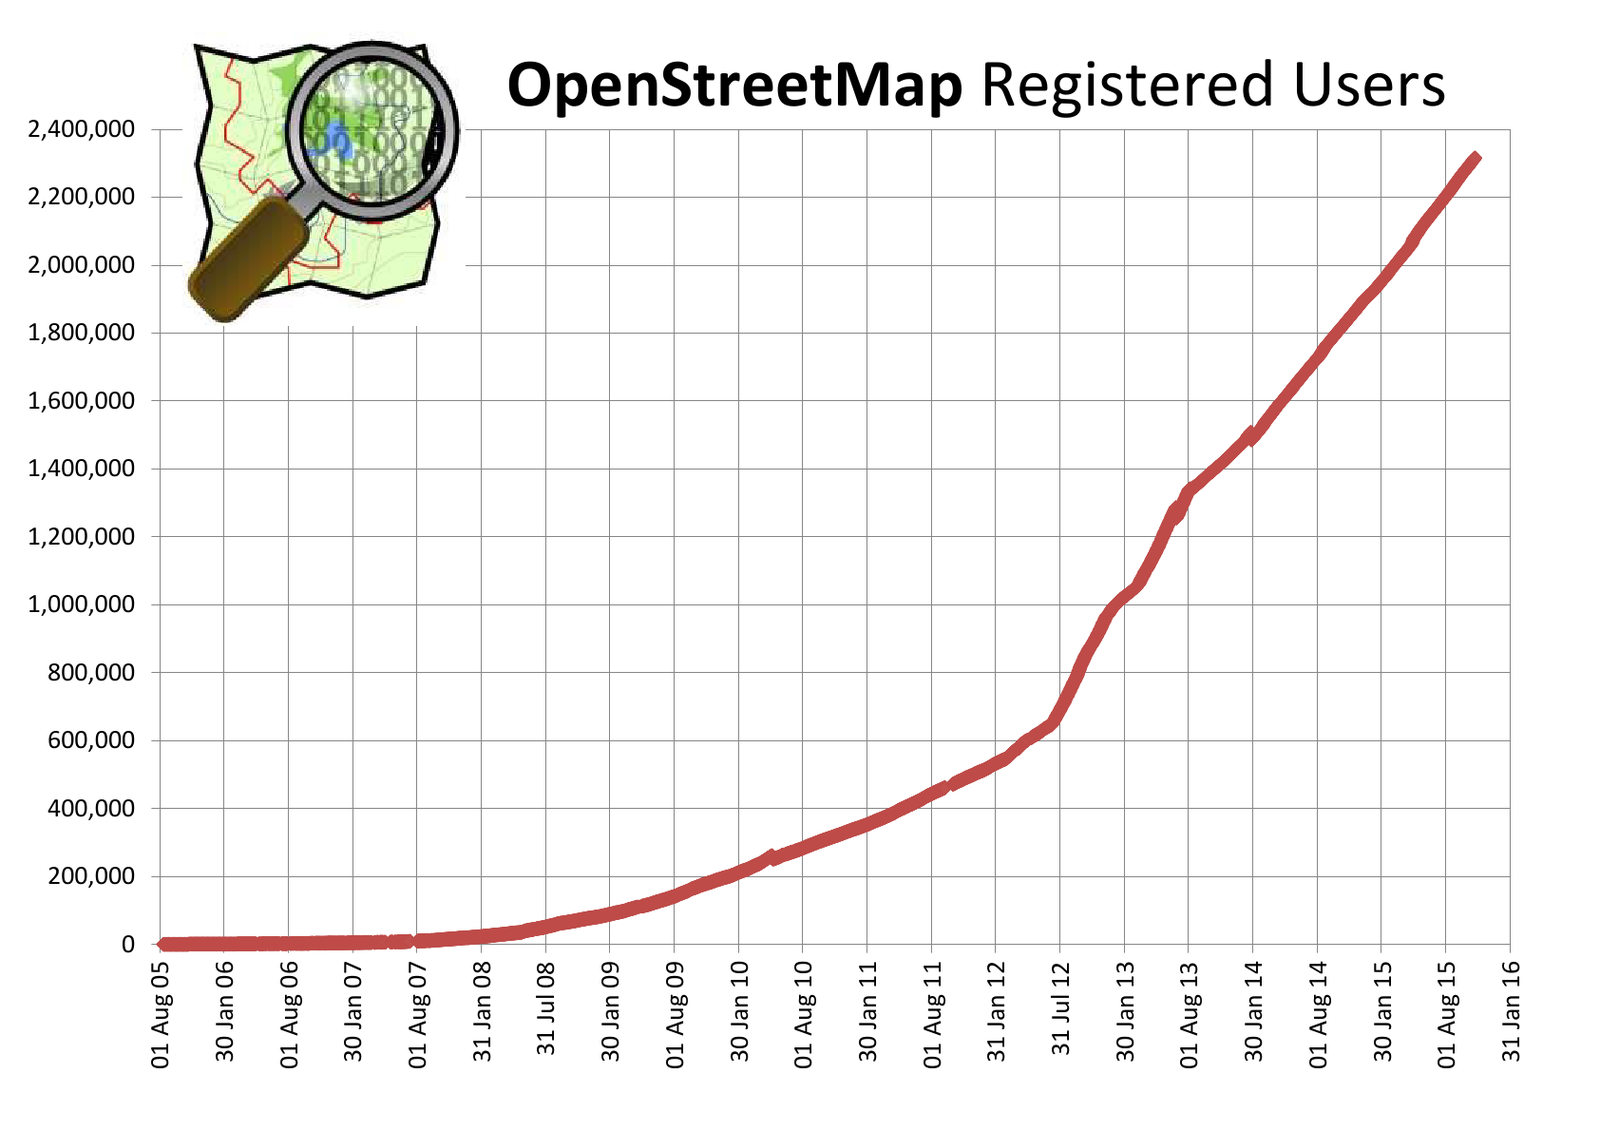
\includegraphics[scale=0.5]{OpenStreetMap/utenti.png}
	\caption{Scala lineare di utenti iscritti ad OpenStreetMap}
	\label{fig:utenti_OSM}
\end{figure}
Nel prossimo paragrafo si illustreranno meglio i motivi dell'esistenza di un progetto come OSM.


\newpage 
\section{Perchè il mondo ha bisogno di OSM} 

Finora quello di OSM sembrerebbe un altro progetto di nobile causa ma fine a se stesso. Per comprendere meglio la sua importanza bisogna fare un passo indietro nella storia e tornare nel 1800 \cite{WHYNEED} .\\
In quel periodo uno dei tanti problemi era costituito dal tempo, non in termini di tempo a disposizione, ma di che ora fosse. Gli orologi esistevano già, ma ogni città aveva il suo "tempo locale". Viene da sé come anche prendere un banale appuntamento con l'amico del paese vicino, comportasse una grande difficoltà. Successivamente l'adozione di uno standard comune ha reso il tempo \textbf{universale, libero e di tutti}.
L'equivalente attuale del dilemma del tempo è la posizione geografica, e diversi soggetti stanno cercando di diventarne il riferimento assoluto (Google spende un miliardo di dollari l'anno per mantenere le proprie mappe). 
Dunque perché il mondo ha bisongo di OSM? La risposta è semplice, perché in una società nessuna azienda dovrebbe avere il monopolio su qualcosa. I luoghi sono un bene comune, e dando ad una o poche entità questo potere gli viene dato non solo il potere di dirti la tua posizione, ma anche di poterla manipolare.
Ci sono tre aspetti da analizzare:
\begin{itemize}
\item Cosa viene visualizzato
\item Dove dovresti andare
\item Privacy personale\\
\end{itemize} 

\textbf{Cosa viene visualizzato:} Chi decide cosa debba essere visualizzato su una mappa di Google? Ovviamente Google. Se pensiamo ad un servizio pubblico, questo deve essere il più imparziale e trasparente possibile, come potrebbe esserlo se utilizza un mappa di Google?.\\
Il punto è, nel momento in cui si sceglie un provider di mappe, gli viene dato il potere di decidere quali siano gli elementi a cui dare risalto, o quali non debbano essere proprio mostrati.\\\\
\textbf{Dove dovresti andare:} La seconda questione riguarda il posizionamento. Chi decide cosa sia più vicino a me? Ancora una volta la risposta è banale. Non è un caso che scrivendo su Google Maps la parola \textit{"colazione"} vengano mostrate le grandi catene come McDonald's piuttosto che il bar sotto casa.\\
Nell'immagine successiva viene mostrato uno screenshot della ricerca \textit{"colazione"} effettuata su Google Maps all'interno della biblioteca di scienze umane dell'universita dell'Aquila. 

\begin{figure}[H]
	\centering
	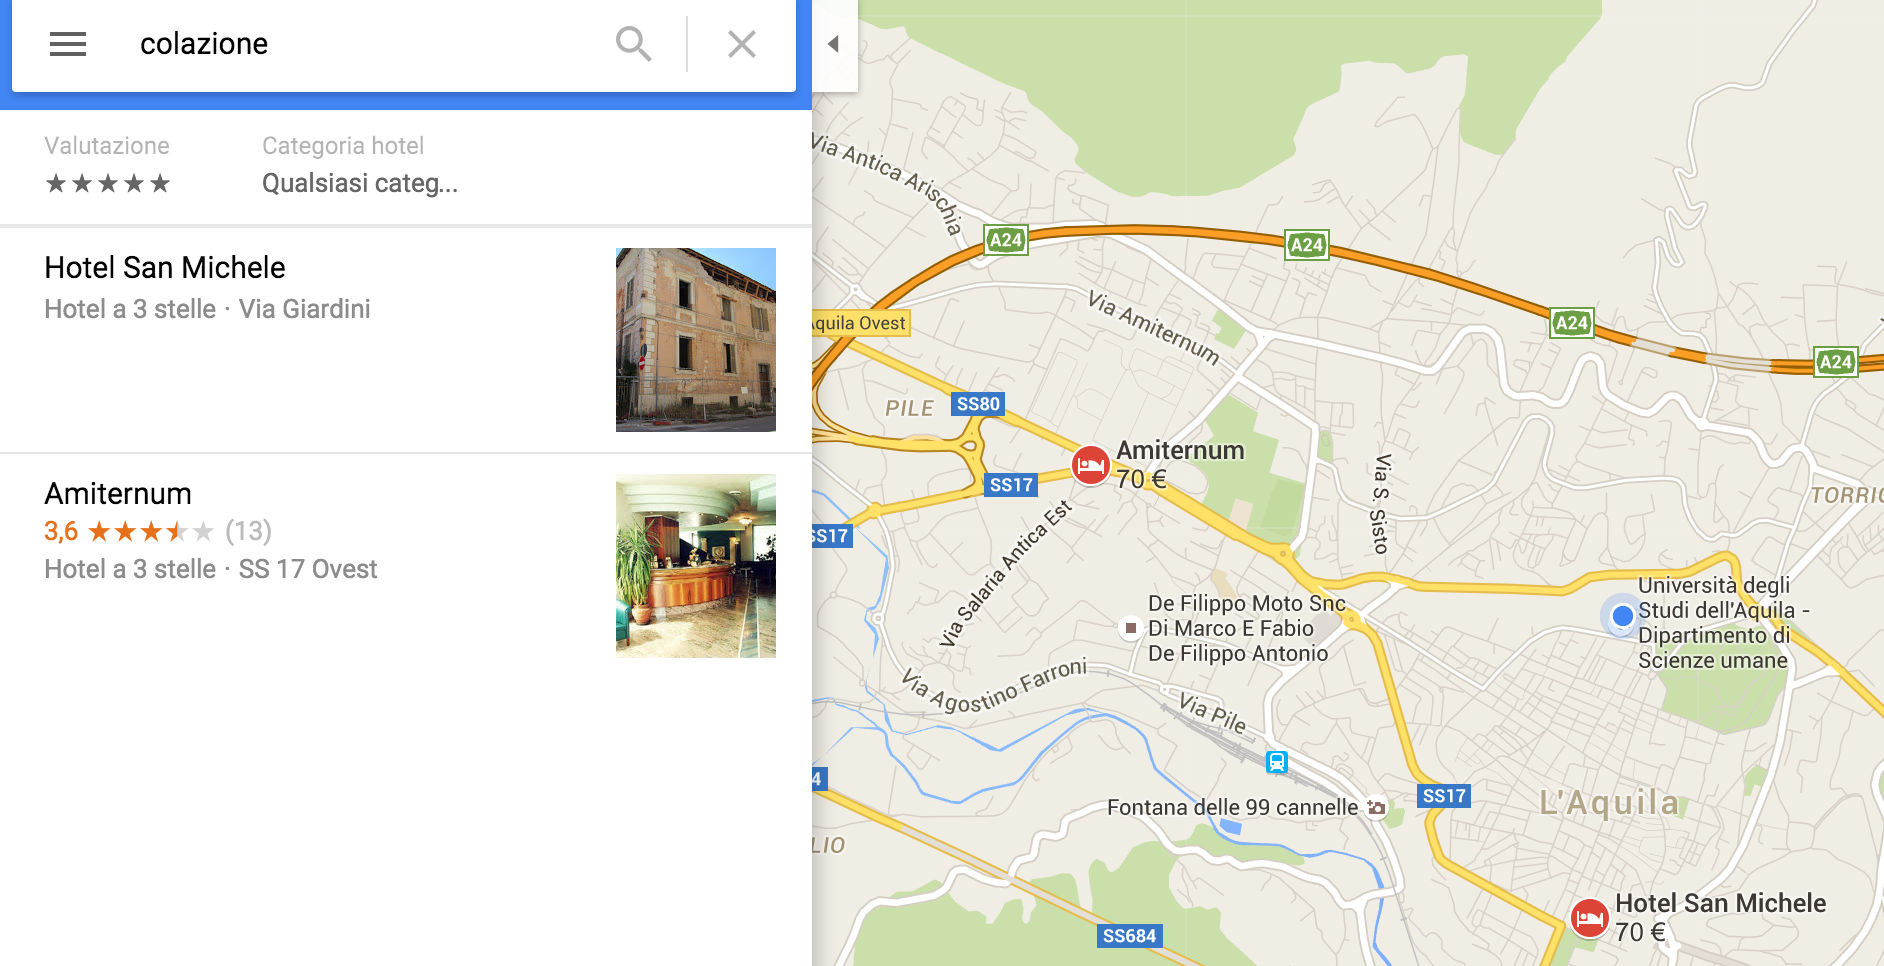
\includegraphics[scale=0.4]{OpenStreetMap/colazione.png}
	\caption{Risultato ricerca "colazione"}
	\label{fig:Ricerca_colazione}
\end{figure}

Come possiano notare vengono mostrati soltanto due hotel locali, che probabilmente hanno pagato il provider, nonostante ci sia un piccolo bar appena fuori la struttura.\\\\
\textbf{Privacy personale:} L'ultima questione riguarda la privacy. Sia Google che Apple raccolgono una quantita smisurata di informazioni sulla posizione degli utenti che utilizzano le loro API. E’ evidente che non si possono ignorare le implicazioni sociali che comporta la disponibilità di così tanti dati in mano ad una singola azienda, indipendentemente da quanto si dichiari benevola.  Aziende come Foursquare utilizzano il mezzo della “gamification” per coprire quello che di fatto è un’opera di acquisizione di dati, e anche Google è entrata nella partita della “gamification” con \textit{Ingress}, un gioco che sovrappone un mondo virtuale a quello reale e porta gli utenti a raccogliere foto e informazioni stradali con l’obiettivo di combattere, o favorire, un’invasione aliena.



\newpage
\section{OpenStreetMap vs Google Maps}
Tralasciando le questioni etiche e al fine della realizzazione dell'applicazione, sono stati analizzati i seguenti topic per la scelta del map-provider:
\begin{itemize}
\item Accuratezza
\item Costo e Download
\item Scalabilità\\
\end{itemize} 

\textbf{Accuratezza:} Poiché le mappe fornite da OSM sono il frutto di lavori "amatoriali", si è indotti a pensare che queste non rispecchino la realtà. Come in ogni progetto in stile wiki, non c'è alcuna garanzia riguardo l'accuratezza dei dati. C'è da dire, però, che quasi nessuna mappa "commerciale" dà alcuna garanzia di accuratezza. In fondo, gli errori intenzionali, sono per l'appunto, errori. \cite{ACCURATEZZA_MAPPE} \\
L'essenza stessa dei processi in stile wiki è che gli utenti stessi, tutti gli utenti, hanno un ruolo nell'accuratezza dei contenuti. Se qualcuno dovesse inserire dati errati, per errore o con intenzione, tutti gli altri possono accorgersene e correggere l'errore o semplicemente eliminarlo. La presenza di una larghissima maggioranza di utenti benintenzionati garantisce che gli errori restino entro un limite accettabile.\\
L'esperienza degli altri progetti basati su wiki ci insegna, comunque, quanto sia agevole raccogliere dati di buona/ottima qualità e quanto, invece, possa essere complicato scovare gli inevitabili errori.
Attualmente non sono stati realizzati processi o meccanismi che rendano semplice questo genere di controllo, tuttavia una comunità attiva come quella di OSM garantisce un controllo qualità sufficiente.\\
La domanda che dobbiamo porci è chi meglio di noi conosce il quartiere dove abitiamo? O la strada che percorriamo tutti i giorni o il parco dove portiamo il nostro animale a passeggiare? La risposta è \textbf{NOI}. Ed è proprio questo sottile concetto a fare la differenza tra una mappa OSM e una mappa proprietaria.\\
Utilizzando uno dei tanti "map-compare" sulla rete possiamo fare degli esempi concreti. Nella Figura 1.4 abbiamo una duplice visualizzazione dell'area universitaria di Coppito (L'Aquila): a sinistra vediamo la mappa ottenuta tramite dati OSM mentre a destra la stessa mappa fornita da Google.

\begin{figure}[H]
	\centering
	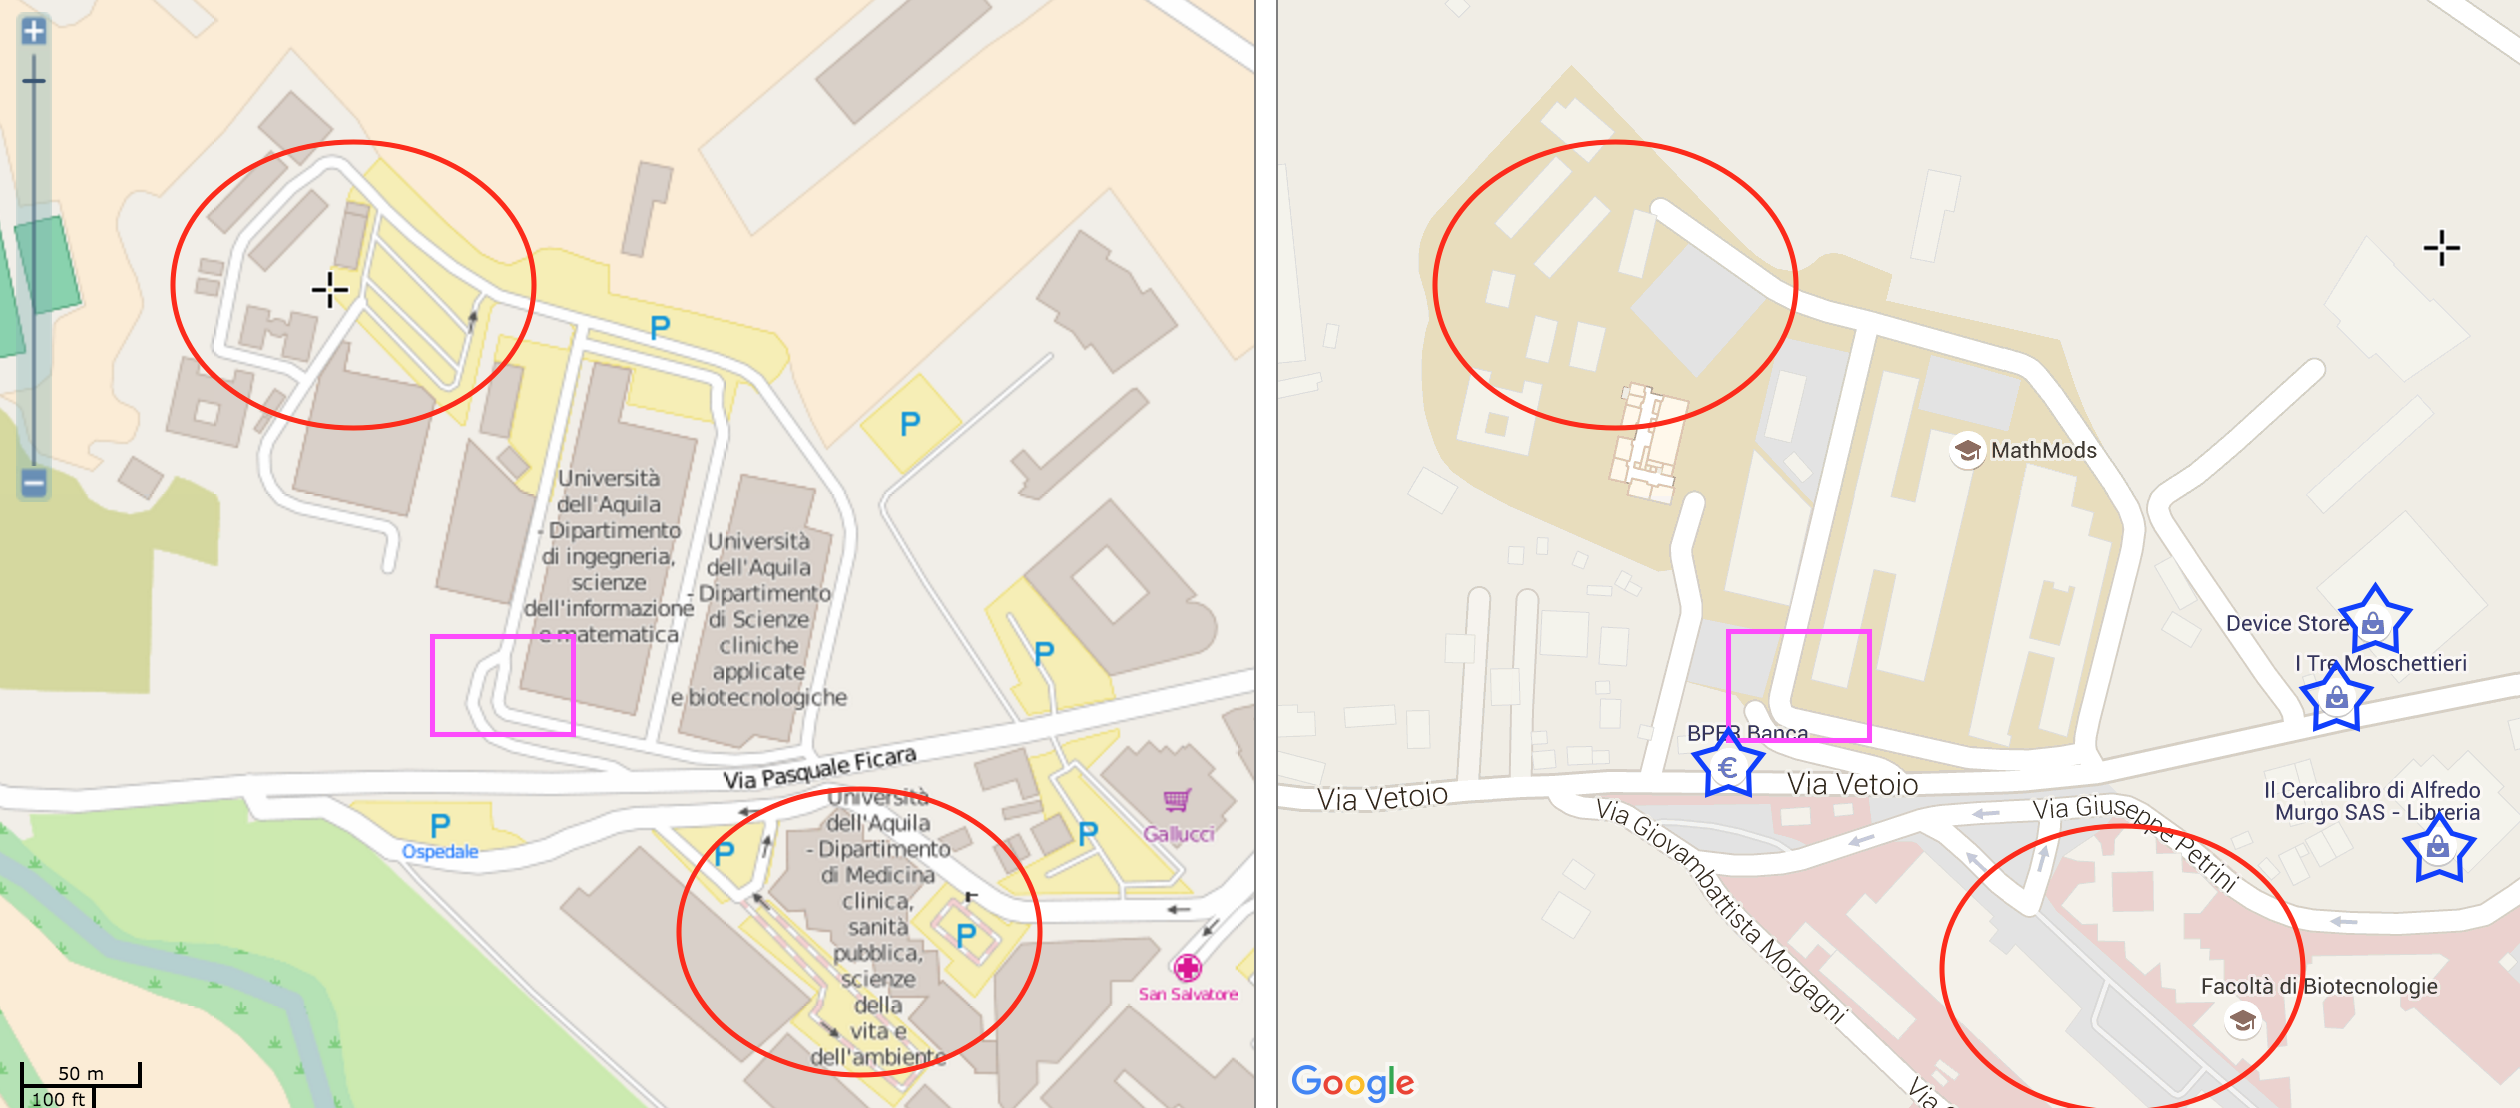
\includegraphics[scale=0.3]{OpenStreetMap/map_compare_coppito.png}
	\caption{Polo universitario di Coppito-L'Aquila}
	\label{fig:Compare_Coppito}
\end{figure}

Soffermiamoci quindi soltanto sulle porzioni di mappa racchiuse nelle diverse figure geometriche:

\begin{itemize}
\item \textbf{Cerchi rossi:} notiamo come nella mappa di Google siano assenti diverse strade interne alla struttura che collegano i diversi edifici tra di loro; questi sono percorribili da un veicolo d'emergenza o più semplicemente un'autovettura.
\item \textbf{Rettangolo viola:} Presenza di un errore (possibile easter eggs) da parte di Google: la strada non si interrompe in quel modo
\item \textbf{Stelle blu:} Presenti solo nella mappa di Google, indicano tutte attività commerciali, sarà un caso?
\end{itemize} 

Infine osservando la mappa fornita da Google non si percepisce di avere davanti una grande struttura universitaria, mentre sulla mappa OSM sono indicati perfino i nomi dei dipartimenti presenti nei diversi edifici. \newpage

\textbf{Costo e download:} Volendo realizzare un'applicazione per dispositivi mobili completamente gratuita, priva di pubblicità o di qualsiasi atra forma di lucro, di questo fattore non si può non tenere conto.
Per quanto riguarda Google, l'API javascript è gratis fino ad un massimo di venticinquemila richieste giornaliere per novanta giorni consecutivi. Superata questa soglia si ha un costo di \$ 0,50 ogni mille richieste \cite{GOOGLE_PLAN}. \\
Oltre al costo vengono applicate le seguenti restrizioni:

\begin{itemize}
\item \textbf{Area limitata:} è possibile scaricare una porzione di mappa la cui dimensione massima non superi i centoventimila chilometri quadrati              \cite{GOOGLE_OFFLINE}.
\item \textbf{Scadenza:} le mappe saranno disponibili in assenza di rete per un totale di 30 giorni, dopodiché si dovrà effettuare l'accesso alla rete.
\end{itemize}

Per quanto riguarda OSM, essendo un progetto open-data, non vi è alcuna restrizione. Infatti, è possibile scaricare l'intera mappa del mondo o porzioni di essa in totale libertà e conservarle a tempo indeterminato \cite{LINK_PLANET}.
\newpage

\textbf{Scalabilità:} Quest'ultimo topic ha segnato di fatto il punto decisivo per la scelta di OSM come map-provider. L'associazione no-profit HOT (Humanitarian Openstreetmap Team), ha lo scopo di fornire un valido supporto sul campo al mapping di aree colpite da disastri ambientali e non.\\
Nel sito ufficiale si possono visualizzare i rapporti delle principali emergenze a cui l'associazione ha partecipato \cite{HOT_PROJECT} , consideriamo quindi il terremoto di Haiti.\\
Il 12 gennaio 2010 un violento terremoto di magnitudo 7.0 Mw (quello che colpi L'Aquila nel 2009 fu di 6.3 Mw) con epicentro localizzato a circa 25 chilometri in direzione ovest-sud-ovest della città di Port-au-Prince, capitale dello Stato caraibico di Haiti, colpì tutta l'area circostante.\\
Il numero di vittime è stato stimato al 24 febbraio 2010 in 222.517. Secondo la Croce Rossa Internazionale e l'ONU, il terremoto avrebbe coinvolto più di 3 milioni di persone \cite{WIKI_HAITI}.\\ Sei ore dopo il disastro la mappa disponibile di Port-au-Prince era la seguente:

\begin{figure}[H]
	\centering
	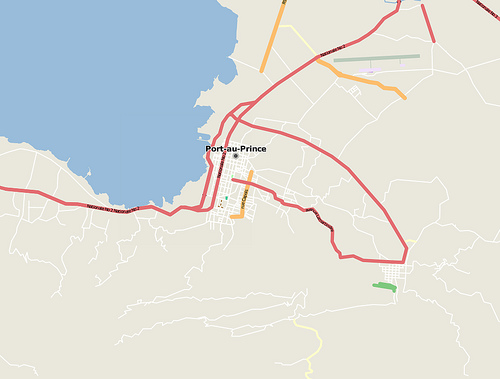
\includegraphics[scale=0.6]{OpenStreetMap/haiti_prima.jpg}
	\caption{Mappa OSM di Pourt-au-Prince 6 ore dopo il terremoto del 2010}
	\label{fig: haiti_day0}
\end{figure}
\newpage
Nelle ore successive, numerose aziende di geo-data (Geo-eye, Google, Yahooo...) resero pubbliche le proprie immagini satellitari, in modo tale che i volontari potessero mappare l'area colpita dal proprio pc in qualsiasi parte del mondo. \\
Quello che avvenne fu qualcosa di straordinario, come disse Jeffery Johnson \textit{"What we did in Haiti changed disaster response forever"}. \\
Il contributo di più di seicento volontari portò ad avere dopo appena 48h dal disastro la seguente mappa:

 \begin{figure}[H]
	\centering
	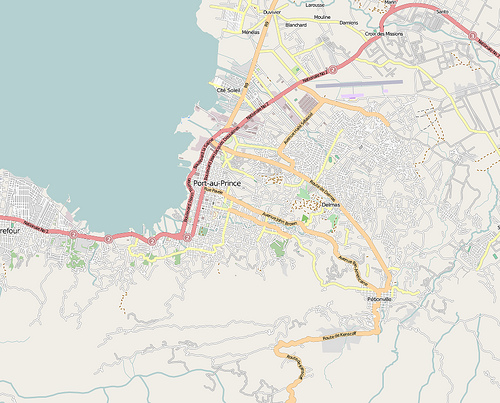
\includegraphics[scale=0.6]{OpenStreetMap/haiti_dopo.jpg}
	\caption{Mappa OSM di Pourt-au-Prince 48 ore dopo il terremoto del 2010}
	\label{fig: haiti_day2}
\end{figure}

La mappa nelle settimane successive continuò ad essere aggiornata e raffinata, tutto questo ha facilitato il coordinamento delle operazioni umanitarie di soccorso e approvigionamento, salvando di fatto innumerevoli vite.\\
In conclusione OSM garantisce un'ottima scalabilità, caratteristica che come abbiamo visto, nei contesti di disaster-management è di fondamentale importanza. 

%\chapter{L'applicazione lato utente}
Nella prima parte di questo capitolo, vengono illustrati i requisiti di sistema che hanno guidato lo sviluppo dell'intera applicazione. Mentre nella parte finale verranno mostrati i task principali e le relative schermate dell'interfaccia realizzata con il framework Ratchet (vedi \ref{ratchet}).
\section{Il concept}
La progettazione dell'applicazione è stata guidata, oltre allo studio di numerosi documenti riguardanti il contesto d'uso, dalla definizione di alcuni concetti chiave. \\
Nel contesto d'uso, le persone sono interessate a conoscere lo stato dei propri cari e di alcuni luoghi d'interesse. Questa osservazione è stata implementata nei concetti di Friends Of Interest e Point Of Interest; i FOI e i POI rappresentano quindi l'insieme delle persone e dei luoghi per i quali l'utente ritiene rilevante conoscere lo stato in uno scenario di disatro ambientale e/o umano.\\
Un'altra questione importante è l'attendibilità delle informazioni mostrate; per questo motivo ogni stato, che sia un FOI o un POI, è correllato dalla data e l'ora in cui è stato "prodotto". Per i POI l'attendibilità è rafforzata dal numero di segnalazioni di tale emergenza; infatti dato che chiunque, tramite una procedura standard, potrebbe segnalare un'emergenza in quello specifico luogo ha senso considerarlo come un buon indice di attendibilità dell'informazione, senza trascurare però quei luoghi (come le case indipendenti) che avranno un numero relativamente più basso di segnalazioni.\\
Per i FOI oltre allo stato, si è pensato di utilizzare una sorta di "ping";  il dispositivo perdiodicamente e in base al numero degli utenti intorno a lui, invia un "bit" al sistema centrale, se allo scadere di un certo timeout, non si hanno notizie del dispositivo verrà considerato come spento. In questo modo gli utenti possono sapere se il dispositivo di un loro caro è spento, acceso o se egli stia usando l'applicazione. 

\section{Requisiti di sistema}
La stesura dei requisiti di sistema è un processo imprenscindibile per la progettazione, nel nostro caso è il risultato di un processo iterativo basato sulla valutazione di un esperto.\\
I requisiti sono divisi in:
\begin{itemize}
\item \textbf{Requisiti funzionali} indicano quello che il sistema deve fare
\item \textbf{Requisiti non funzionali} vincoli sul sistema e il suo sviluppo
\end{itemize}
 
 \subsection{Requisiti funzionali}

\begin{enumerate}
\item Interazione mappa
  \begin{itemize}
     \item\textit{Identificativo:} RF-1
  \item\textit{Descrizione:} Il sistema deve permettere all’utente di interagire con la mappa, compiendo le azioni basilari quali: zoom In, zoom Out, CCW (Change Center View), click.
  \end{itemize}
  \newpage
\item Impostazione POI
  \begin{itemize}
  \item\textit{Identificativo:} RF-2
  \item\textit{Descrizione:} Il sistema deve permettere all’utente di impostare una specifica porzione di mappa come un POI (point of interest).
  \item\textit{Razionale:} In questo modo l’utente può applicare un filtro sulla mappa (vedi RF-7)  e visualizzare rapidamente lo status dei luoghi d’interesse.
  \end{itemize}
  
\item Impostazione FOI
  \begin{itemize}
  \item\textit{Identificativo:} RF-3
  \item\textit{Descrizione:} Il sistema deve permettere all’utente di impostare altri utenti del sistema come FOI (Friends Of Interest).
  \item\textit{Razionale:} l’utente può in questo modo applicare un filtro (vedi RF-7) e visualizzare in modo rapido lo status delle persone d’interesse.
  \end{itemize}
  
  \item Segnalazione evento
  \begin{itemize}
  \item\textit{Identificativo:} RF-4
  \item\textit{Descrizione:} l’utente deve poter segnalare la posizione di un certo evento (vedi RNF-1). 
La procedura standard di segnalazione deve avvenire sia cliccando su un punto della mappa sia tramite una schermata dedicata.
Nel caso di rete congestionata o assente il sistema deve provvedere alla bufferizzazione delle richieste e avvisare di tale situazione l’utente stesso.
  \item\textit{Razionale:} In questo modo gli utenti contribuiscono all’aggiornamento dello status generale del territorio colpito.
  \end{itemize}
  
   \item Aggiornamento status
  \begin{itemize}
  \item\textit{Identificativo:} RF-5
  \item\textit{Descrizione:} L’utente può cambiare il suo status (vedi RNF-4). Il sistema quindi deve comunicare immediatamente al server tale aggiornamento.
  \item\textit{Razionale:} In questo modo gli utenti contribuiscono a fornire informazioni dinamiche sul territorio colpito e su se stessi.
  \end{itemize}
  
  \item Trusty data
  \begin{itemize}
  \item\textit{Identificativo:} RF-6
  \item\textit{Descrizione:} Il sistema deve informare l’utente sul grado di aggiornamento delle informazioni visualizzate, ovvero:
    \begin{itemize}
    \item Eventi
    \item Status dei POI
    \item Status dei FOI
    \item mappe offline
    \end{itemize}
   L’attendibilità degli eventi è data dal numero di segnalazioni di tale evento nella relativa cella (vedi RNF-1) e dall’orario in cui è stata generata l’ultima    segnalazione.
   \item\textit{ Razionale:} Nel contesto d’uso, la rete potrebbe collassare o più semplicemente gli utenti potrebbero non utilizzare il sistema per un certo periodo, in questo modo si garantisce la totale trasparenza delle informazioni fornite.
  \end{itemize}
  
  \item Filtra mappa
  \begin{itemize}
  \item\textit{Identificativo:} RF-7
  \item\textit{Descrizione:} Il sistema deve permettere all’utente di filtrare le informazioni visibili sulla mappa in base a:
    \begin{itemize}
    \item propri POI
    \item tipo eventi
    \item propri FOI
    \end{itemize}
   \item\textit{Razionale:} La mappa visualizzata dall’utente potrebbe contenere un numero elevato di informazioni.
  \end{itemize}
  
    \item Modalità offline
  \begin{itemize}
  \item\textit{Identificativo:} RF-8
  \item\textit{Descrizione:} Il sistema deve salvare porzioni di mappa visualizzate dall’utente attraverso l’interazione base (vedi RF-1) nella memoria temporale, inoltre l’utente deve poter scaricare una specifica center view su diversi livelli di zoom. Il sistema quindi deve permettere all’utente di utilizzare la modalità offline, in questo caso la rete verrà utilizzata solamente per inviare e ricevere aggiornamenti riguardo:
    \begin{itemize}
    \item POI e NPOI
    \item FOI e NFOI
    \item Eventi
    \end{itemize}
   \item\textit{Razionale:} L’utente potrebbe voler utilizzare la modalità offline per risparmiare dati o per la  pessima connessione
  \end{itemize}
  
   \item Markercluster
  \begin{itemize}
  \item\textit{identificativo:} RF-9
  \item\textit{Descrizione:} Il sistema per livelli di zoom, sufficientemente bassi, deve raggruppare i marker in un unico markercluster; inoltre deve mostrare la quantità di elementi inglobati.
  \end{itemize}
  
    \item Aggiornamento dati persistenti
  \begin{itemize}
  \item\textit{identificativo:} RF-10
  \item\textit{Descrizione:} Il sistema deve periodicamente richiedere al server l’aggiornamento dei dati persistenti (vedi RNF-2).
Inoltre l’utente può richiedere l’aggiornamento in qualsiasi momento
  \end{itemize}
  
   \item Salta a
  \begin{itemize}
  \item\textit{Identificativo:} RF-11
  \item\textit{Descrizione:} Il sistema deve permettere all’utente di spostare la propria center view al NPOI (nearest point of interest), al NFOI (nearest family of interest) o al riferimento di una notifica d’allerta (vedi RF-11) cliccando su di essa.
   \item\textit{Razionale:} L’utente potrebbe voler prestare soccorso al famigliare o visualizzare lo status del punto d’interesse più vicino a lui.
  \end{itemize}
  
   \item Notifiche di allerta
  \begin{itemize}
  \item\textit{Identificativo:} RF-12
  \item\textit{Descrizione:} Il sistema deve notificare l’utente sull’aggiornamento dello status di un FOI o della segnalazione di un evento all’interno di un POI.
  \end{itemize}
  
\end{enumerate}

 \subsection{Requisiti non funzionali}
 
\begin{enumerate}
   \item Dati griglia
  \begin{itemize}
  \item\textit{Identificativo:} RNF-1
  \item\textit{Descrizione:} la mappa è divisa da una griglia con celle di 22x16 mt (vedi \ref{santiago}).
   \item\textit{Razionale:} Più utenti vicini potrebbero utilizzare il sistema, senza tolleranza una porzione di mappa potrebbe essere saturata dalla  visualizzazione di eventi omogenei.
  \end{itemize}
  
  \item Dati persistenza
  \begin{itemize}
  \item\textit{Identificativo:} RNF-2
  \item\textit{Descrizione:} il sistema deve memorizzare in modo permanente, attraverso un database locale, i seguenti dati:
	\begin{itemize}
	\item FOI
	\item POI
	\item eventi visualizzati nella center view
	\item porzioni di mappa
	\end{itemize}
  \end{itemize}
  
    \item Dati aggiornabili
  \begin{itemize}
  \item\textit{Identificativo:} RNF-3
  \item\textit{Descrizione:} I dati memorizzati (vedi RNF-2) sono aggiornabili secondo le modalità precedentemente descritte (vedi RF-9).
  \item\textit{Razionale:} Le informazioni cambiano dinamicamente, alcune emergenze potrebbero essere state risolte, altre potrebbero nascere successivamente.
  \end{itemize}
  \newpage
  \item Dati tipi
  \begin{itemize}
  \item\textit{Identificativo:} RNF-4
  \item\textit{Descrizione:} L’utente può scegliere il tipo di evento da segnalare (vedi RF-5) tra i seguenti:
	\begin{itemize}
	\item edificio crollato
	\item incendio 
	\item allagamento
	\item strada interrotta
	\item persona intrappolata
	\item persona ferita
	\item persona non autosufficiente
	\end{itemize}
	Inoltre può scegliere il suo status, che verrà notificato agli utenti che lo hanno impostato come FOI, tra:
	\begin{itemize}
	\item sto bene
	\item ferito lieve
	\item ferito
	\item intrappolato
	\item intrappolato e ferito
	\end{itemize}
  \end{itemize}
 
    \item Ambientale tecnico
  \begin{itemize}
  \item\textit{Identificativo:} RNF-5
  \item\textit{Descrizione:} Il sistema è un’applicazione per dispositivi mobili cross platform, si utilizza il framework phonegap e le tecnologie proprie alla programmazione web:
  \begin{itemize}
  \item HTML
  \item CSS
  \item Javascript
  \end{itemize}
E’ richiesto l’accesso alla rete internet e l’utilizzo del gps integrato del dispositivo
  \end{itemize}
 \newpage
\item Ambientale sociale
  \begin{itemize}
  \item\textit{Identificativo:} RNF-6
  \item\textit{Descrizione:} I dati sono prodotti dagli utenti che attraverso il sistema cooperano per arricchire il server di informazioni vitali sul territorio colpito. Essendo quindi un processo distribuito particolare attenzione deve essere posta all controllo dell’attendibilità degli eventi segnalati per tutti gli utenti (vedi RNF-1)
  \end{itemize}

  \item Ambientale fisico
  \begin{itemize}
  \item\textit{Identificativo:} RNF-7
  \item\textit{Descrizione:} Il sistema potrebbe essere utilizzato in svariati contesti d’uso, di seguito i più comuni:
	\begin{itemize}
	\item assenza di luce
	\item presenza di folla
	\item Scarsa visibilità
	\item forti raffiche di vento
	\item allagamenti
	\item incendi
	\end{itemize}
    \item\textit{Razionale:} Essendo un sistema il cui obiettivo principale è fornire un supporto utile ai soccorritori nel caso di eventi catastrofici, i contesti d’uso dell’applicazione possono essere imprevedibili. Tuttavia si può rispondere al meglio attraverso una buona progettazione del sistema, utilizzando i principi dell’interaction design.
  \end{itemize}
  
\item Utenti
  \begin{itemize}
  \item\textit{Identificativo:} RNF-8
  \item\textit{Descrizione:} la fascia di utenti del sistema è molto ampia, non è possibile stabilirne con certezza gli estremi.
  \end{itemize}
  
  \item Usabilità
  \begin{itemize}
  \item\textit{Identificativo:} RNF-9
  \item\textit{Descrizione:}Il sistema deve essere il più usabile possibile, nel contesto d’uso gli utenti potrebbero essere spaventati o perdere lucidità
  \end{itemize}
  
\end{enumerate}

\section{L'interfaccia grafica}
Nella realizzazione dell'interfaccia si sono utilizzati pattern mobile ormai consolidati come: le liste per  i FOI e i POI, i segment controll per la scelta della loro visualizzazione e la title-bar con icona per tornare alla home.\\
Le gestures non possono essere complicate, infatti come detto nei requisiti la fascia di utenti è molto ampia e alcuni di essi potrebbero avere poca familiarità nell'utilizzo dei dispositivi mobili. Di fatto l'unica gestures presente è il classico "tap" su display touchscreen, scelta che impone un "comportamento a bottone" di tutti gli elementi grafici.\\
In questo paragrafo verranno quindi illustrati i task principali e le relative schermate mostrate dall'applicazione. \\

 \textbf{Dashboard:} è la home del sistema, da qui l'utente può accedere a tutte le sue funzionalità. E' costituita da cinque "blocchi logici", il primo include la title-bar (presente in ogni schermata dell'applicazione), il secondo è composto da un  container con le informazioni sul FOI più grave, il terzo include i due bottoni per i task \textit{"how are you?"} e \textit{"signal event"}, il quarto blocco è composto dall'ultima notizia ufficiale comunicata dai soccorrittori e infine il quinto blocco è costituito da tre bottoni per l'accesso ai FOI, POI e alla mappa.
   \begin{figure}[H]
   
	\centering
	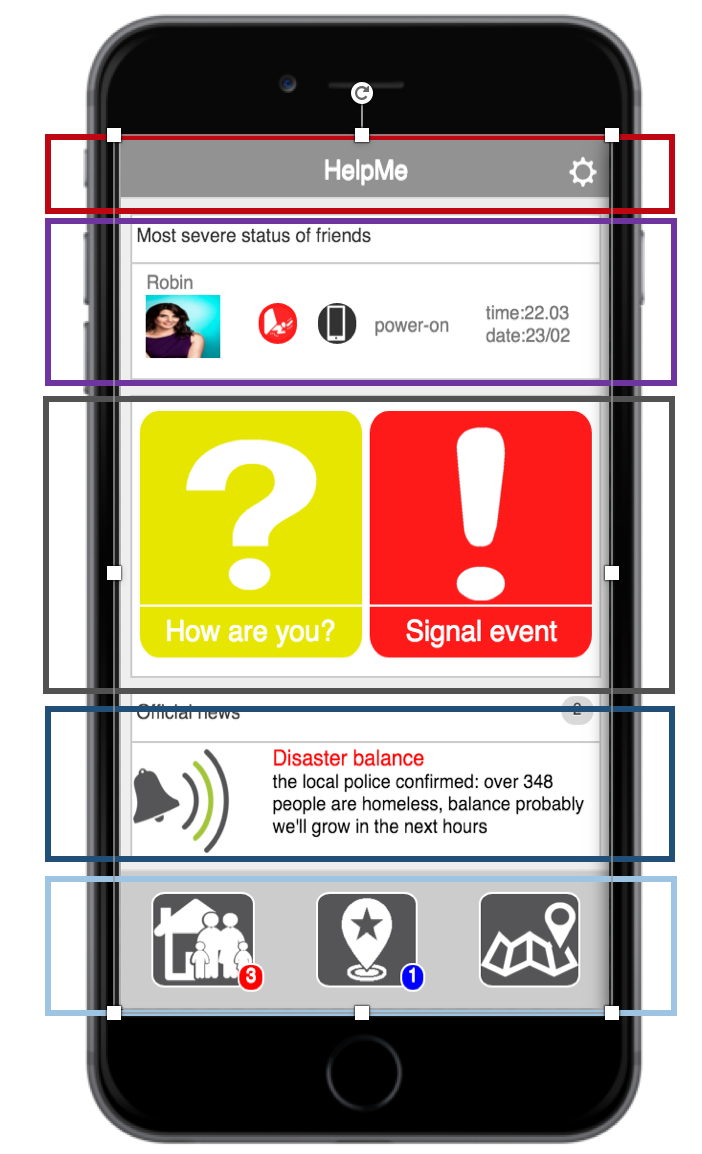
\includegraphics[scale=0.7]{interfaccia/dash.png}
	\caption{Dashboard}
	\label{fig:logo_OSM}
\end{figure}


 
\begin{figure}
\textbf{How are you?:} Per aggiornare il proprio stato bisogna cliccare sul bottone giallo, come in Fig \ref{fig:buttoncomestai}, quindi tappare su un elemento della lista (Fig \ref{fig:lista}). Per rendere effettivo il nostro aggiornamento basterà cliccare sul tasto in alto a destra:\textit{"Publish"}.
\\ \\ \\
 \begin{minipage}[b]{6cm}
   \centering
  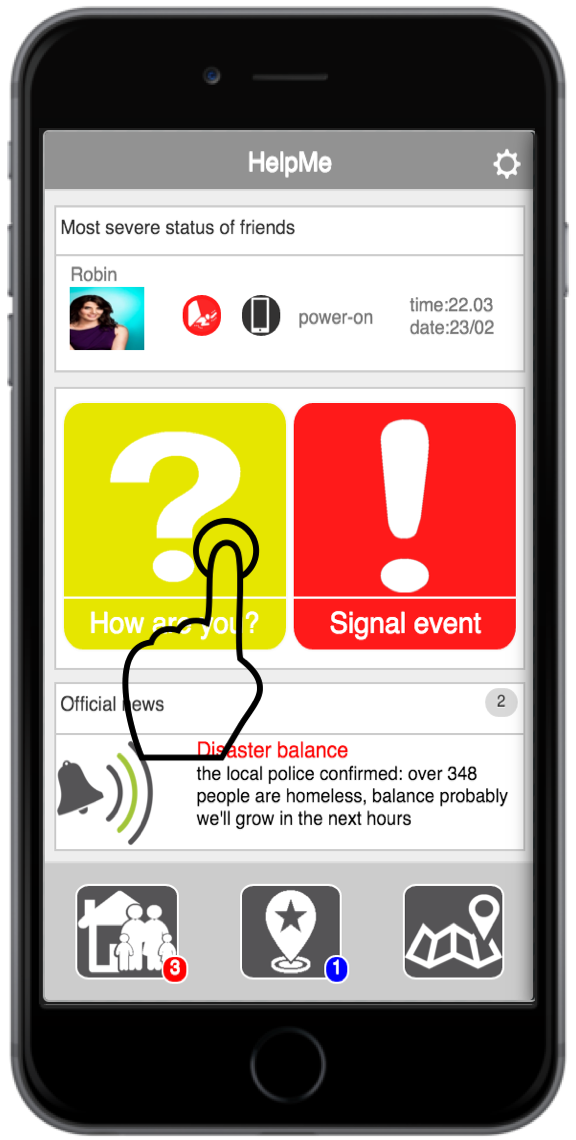
\includegraphics[scale=0.6]{interfaccia/tapbuttoncomestai.png}
	\caption{Tap bottone \textit{"How are you?"}}
	\label{fig:buttoncomestai}
 \end{minipage}
 \ \hspace{6 mm} \hspace{7 mm} \
 \begin{minipage}[b]{6cm}
  \centering
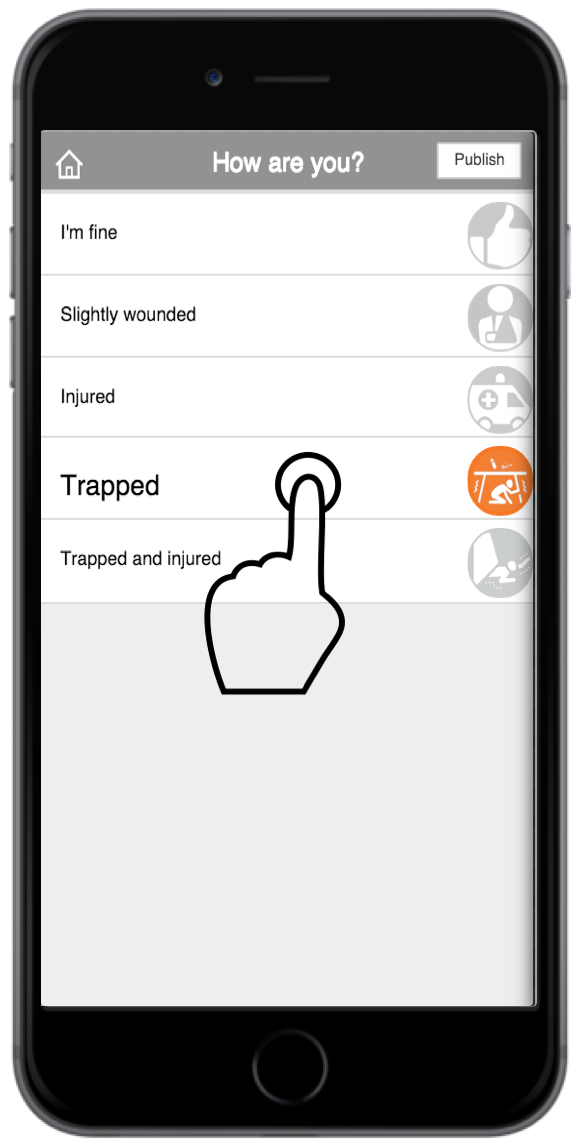
\includegraphics[scale=0.6]{interfaccia/comestaitap.png}
	\caption{Lista predefinita di stati selezionabili}
	\label{fig:lista}
 \end{minipage}
\end{figure}

\newpage


 \begin{figure}
  \textbf{Signal event:} Per segnalare un'emergenza bisogna cliccare, nella dashboard, sul bottone rosso come in Fig \ref{fig:buttonsegnala}. Come per gli stati possiamo scegliere l'emergenza da segnalare da una lista predefinita( Fig \ref{fig:lista-em}).
 \\ \\
 \begin{minipage}[b]{6cm}
   \centering
 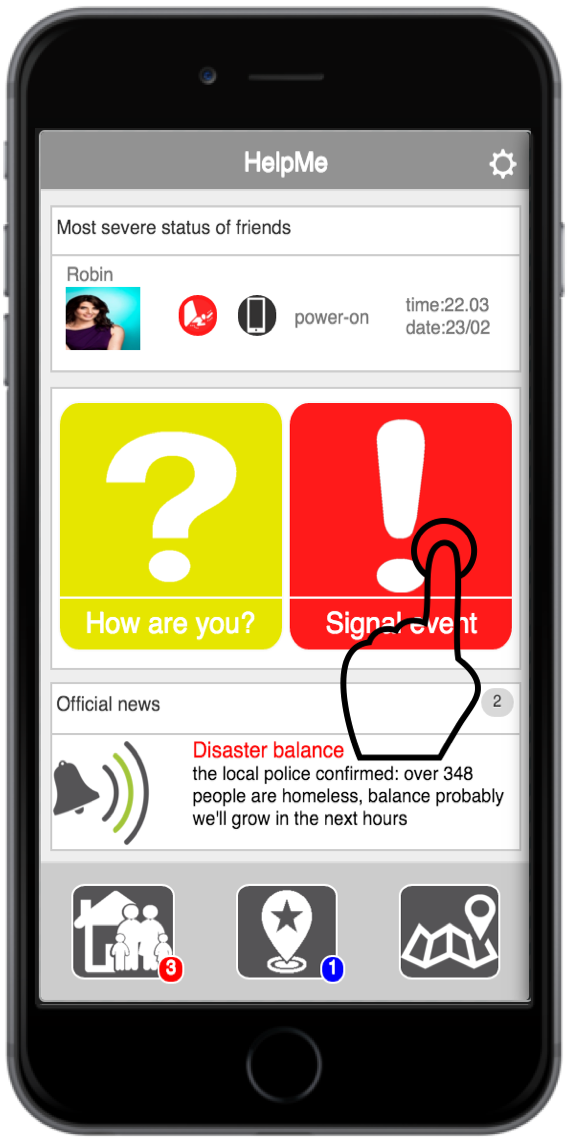
\includegraphics[scale=0.6]{interfaccia/tapbuttonsegnala.png}
	\caption{Tap del bottone \textit{"Signal event"}}
	\label{fig:buttonsegnala}
 \end{minipage}
 \ \hspace{6 mm} \hspace{7 mm} \
 \begin{minipage}[b]{6cm}
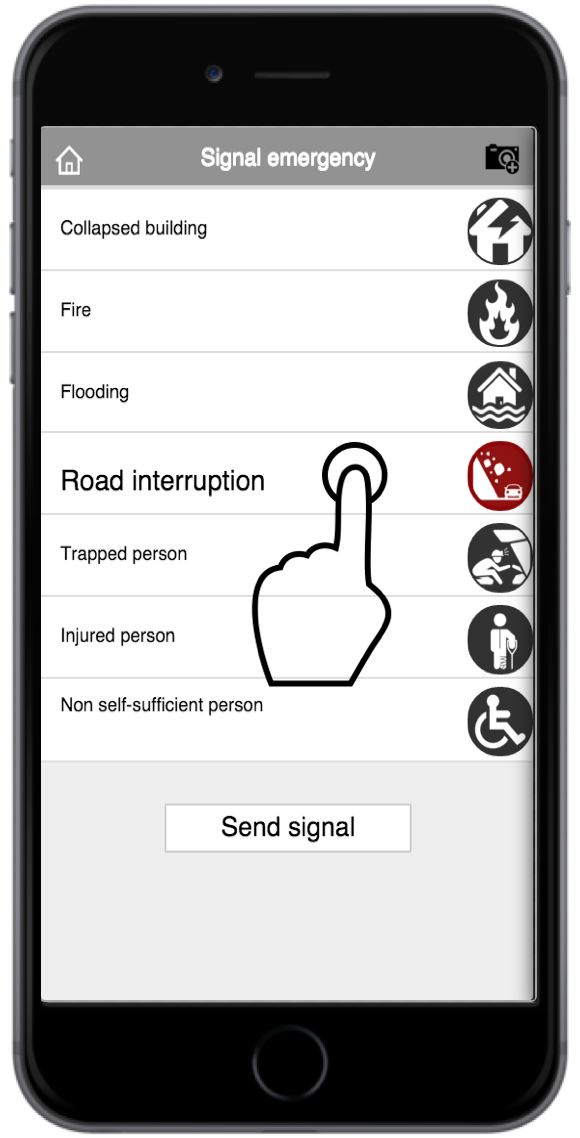
\includegraphics[scale=0.6]{interfaccia/segnalatap.png}
	\caption{Lista predefinita dell'emergenze}
	\label{fig:lista-em}
	
 \end{minipage}
 \\ \\ \\
Quindi premendo sul bottone \textit{"Send signal"}, avremo la possibilità di usare la nostra posizione oppure di utilizzare la mappa (Fig \ref{fig:sceltamappa}).
\end{figure}




 \begin{figure}
\textbf{Where?:} se si decide di utilizzare la mappa per segnalare la posizione dell'emergenza, tappando come in Fig \ref{fig:sceltamappa}, allora si dovrà cliccare su un punto della mappa che il sistema ci mostrerà (Fig \ref{fig:mappa-segnala}).
 \\ \\
 \begin{minipage}[b]{6cm}
   \centering
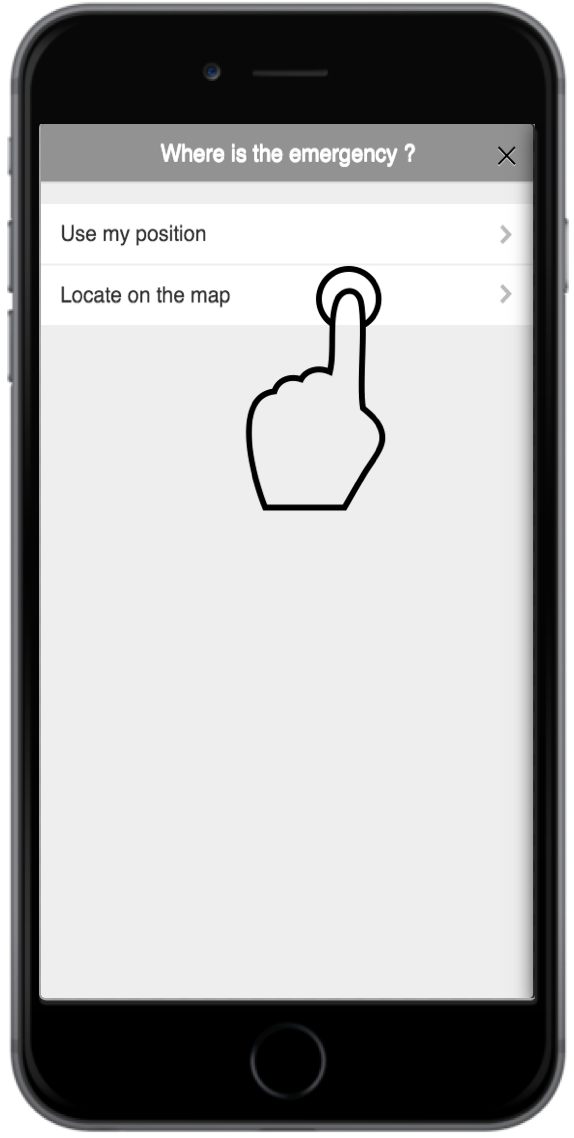
\includegraphics[scale=0.6]{interfaccia/sceltamap.png}
	\caption{Tap \textit{"locate on the map"} }
	\label{fig:sceltamappa}
 \end{minipage}
 \ \hspace{6 mm} \hspace{7 mm} \
 \begin{minipage}[b]{6cm}
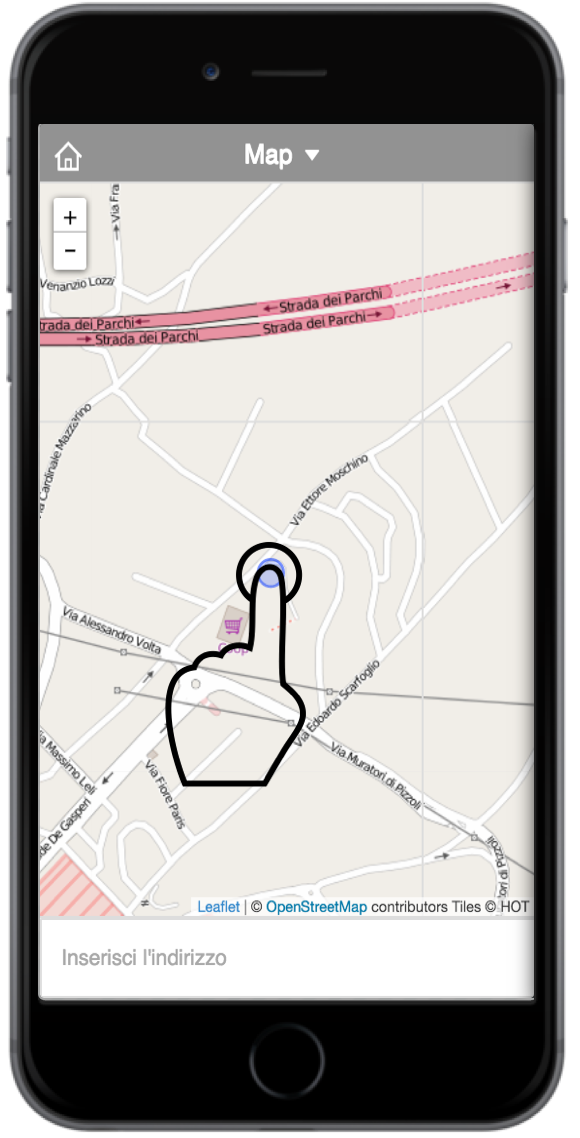
\includegraphics[scale=0.6]{interfaccia/mappasegnala.png}
	\caption{Mappa mostrata dal sistema }
	\label{fig:mappa-segnala}
	
 \end{minipage}
 \\ \\ \\
Per confermare la posizione scelta, basterà infine cliccare sul tasto \textit{"Done"} e segnalare così l'emergenza. 
\end{figure}



 \begin{figure}
\textbf{Visualizza FOI:} per visualizzare lo stato dei nostri cari bisogna tappare, nella schermata della dashboard, il bottone in basso a sinistra come in Fig \ref{fig:tapfoi}. La lista sarà ordinata per default in base alla gravità del loro stato. \\
 Come possiamo vedere in Fig \ref{fig:lista-foi}, ogni elemento (FOI) è composto da un'icona del suo stato correlata dall'ora e la data in cui egli ha eseguito l'aggiornamento, lo stato del dispositivo ottenuto mediante un "ping" del sistema centrale e infine dalla distanza tra lui e l'utente dell'applicazione.
 \\ \\
 \begin{minipage}[b]{6cm}
   \centering
	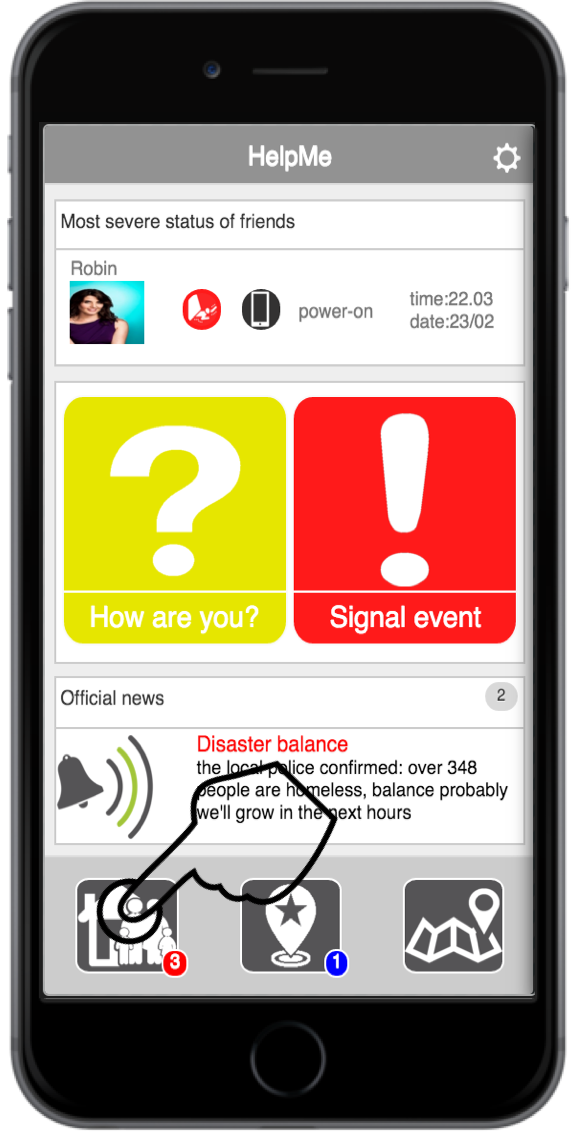
\includegraphics[scale=0.6]{interfaccia/tapfoi.png}
	\caption{Tap da fare per accedere alla lista dei FOI }
	\label{fig:tapfoi}
 \end{minipage}
 \ \hspace{6 mm} \hspace{7 mm} \
 \begin{minipage}[b]{6cm}
\centering
	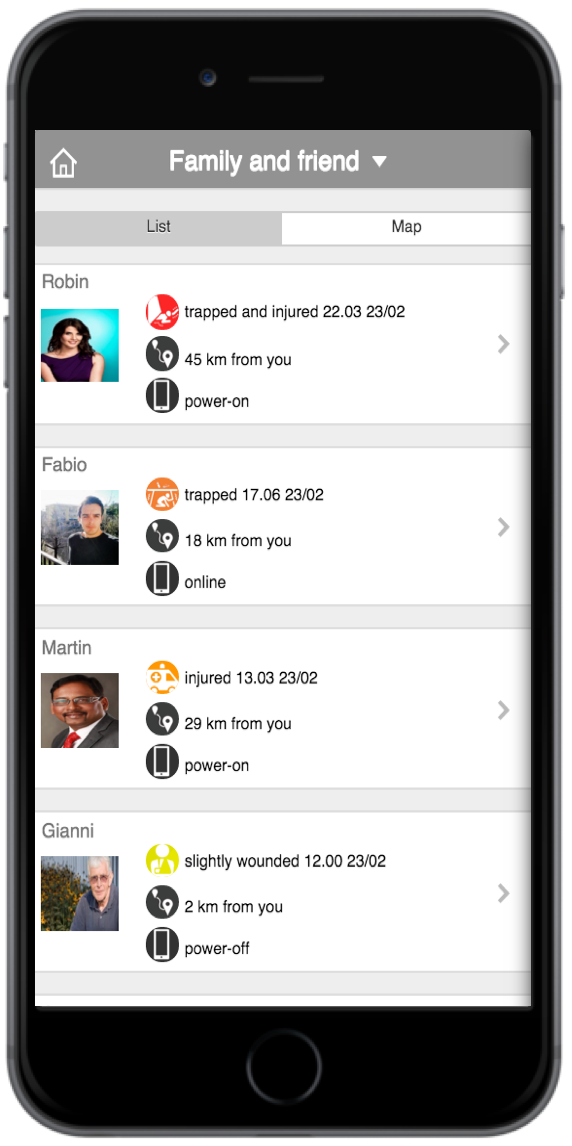
\includegraphics[scale=0.6]{interfaccia/listafoi.png}
	\caption{Lista dei FOI ordinata per default in base alla gravità }
	\label{fig:lista-foi}
 \end{minipage}
\end{figure}


 \begin{figure}
 \textbf{Ordina FOI:} come detto, la lista dei nostri FOI sarà ordinata inizialmente in base alla gravità del loro stato, tuttavia è possibile ordinarla anche a seconda della vicinanza o del più recente aggiornamento semplicemente cliccando prima sull'icona del menu a comparsa, Fig \ref{fig:comparsa}, poi sulla relativa etichetta (Fig \ref{fig:etichetta}).
 \\ \\
 \begin{minipage}[b]{6cm}
   \centering
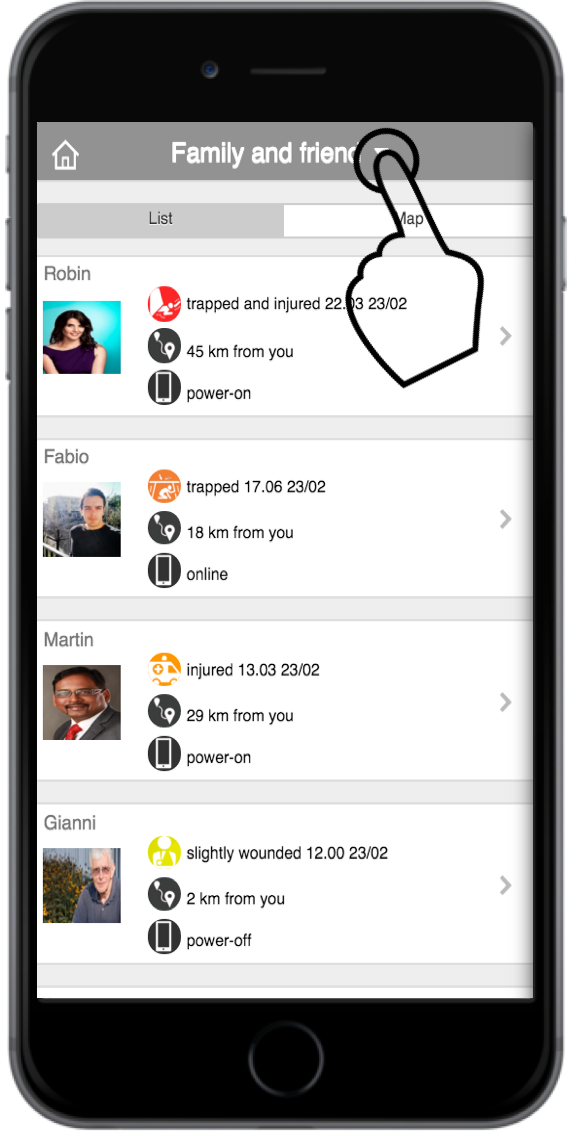
\includegraphics[scale=0.6]{interfaccia/comparsa.png}
	\caption{Tap per aprire il menu a comparsa }
	\label{fig:comparsa}
 \end{minipage}
 \ \hspace{6 mm} \hspace{7 mm} \
 \begin{minipage}[b]{6cm}
\centering
	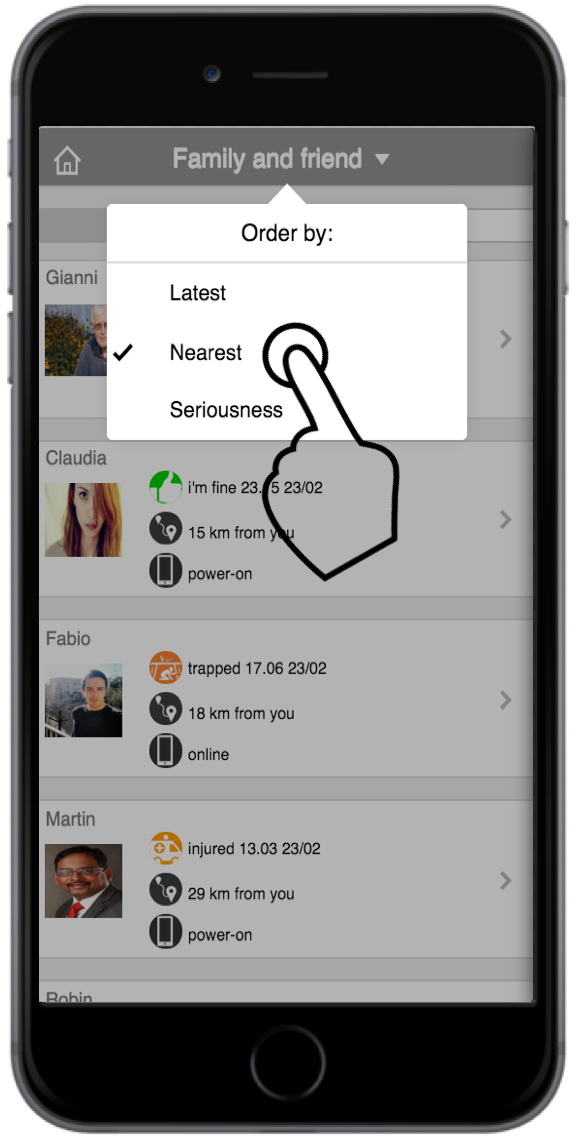
\includegraphics[scale=0.6]{interfaccia/etichetta.png}
	\caption{Tap da fare per ordinare la lista secondo i tre parametri }
	\label{fig:etichetta}
 \end{minipage}
\end{figure}

 \begin{figure}
 \textbf{Visualizza FOI sulla mappa:} oltre alla lista, è possibile visualizzare i propri FOI sulla mappa. Nella schermata precedente basta cliccare sul bottone \textit{"Map"}, come in Fig \ref{fig:mapfoi}. La mappa verrà quindi centrata sul primo FOI della lista, nell'esempio di Fig \ref{fig:mappafoi} la mappa era stata ordinata per \textit{"vicinanza"}.
 \\ \\
 \begin{minipage}[b]{6cm}
   \centering
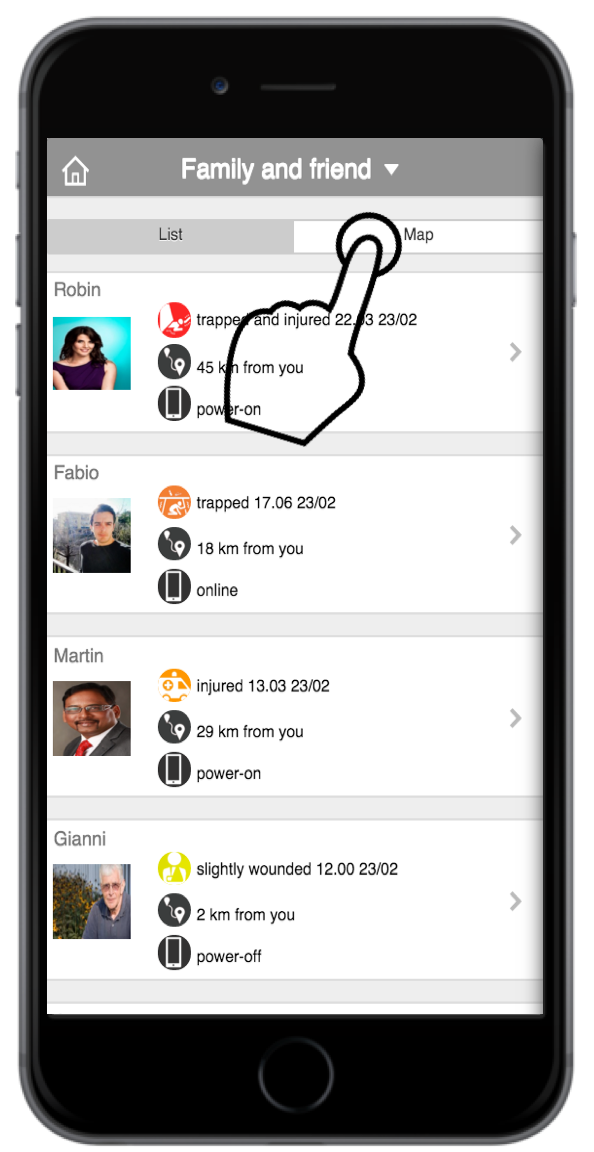
\includegraphics[scale=0.6]{interfaccia/mapfoi.png}
	\caption{Tap per visualizzare i FOI sulla mappa }
	\label{fig:mapfoi}
 \end{minipage}
 \ \hspace{6 mm} \hspace{7 mm} \
 \begin{minipage}[b]{6cm}
\centering
	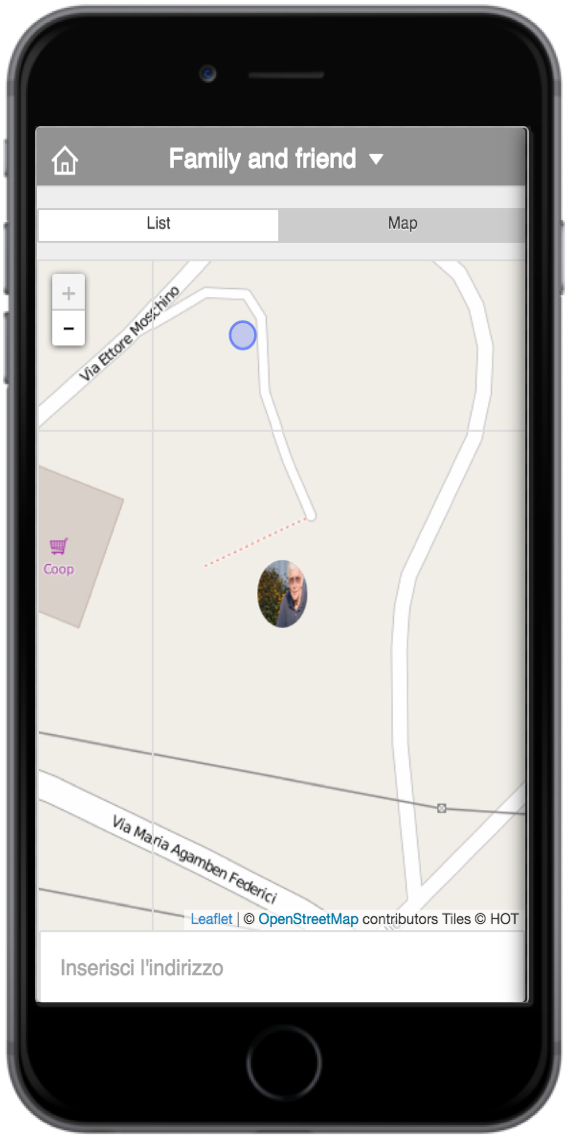
\includegraphics[scale=0.6]{interfaccia/mappafoi.png}
	\caption{Mappa centrata sul FOI più vicino }
	\label{fig:mappafoi}
 \end{minipage}
 \\ \\
E' possibile comunque, con le stesse modalità della lista, centrare la visuale della mappa in base al FOI più vicino, più grave o che abbia aggiornato più recentemente il suo stato
\end{figure}



 \begin{figure}
 \textbf{Clustermarker FOI:} come specificato nei requisiti, i marker dei FOI (e dei POI) devono essere raggruppati quando lo zoom della mappa è tale da farli "toccare" (Fig \ref{fig:markercluster}). Inoltre cliccando il clustermarker è possibile vedere da quali FOI è composto (Fig \ref{fig:markerfoi}). 
 \\ \\
 \begin{minipage}[b]{6cm}
   \centering
	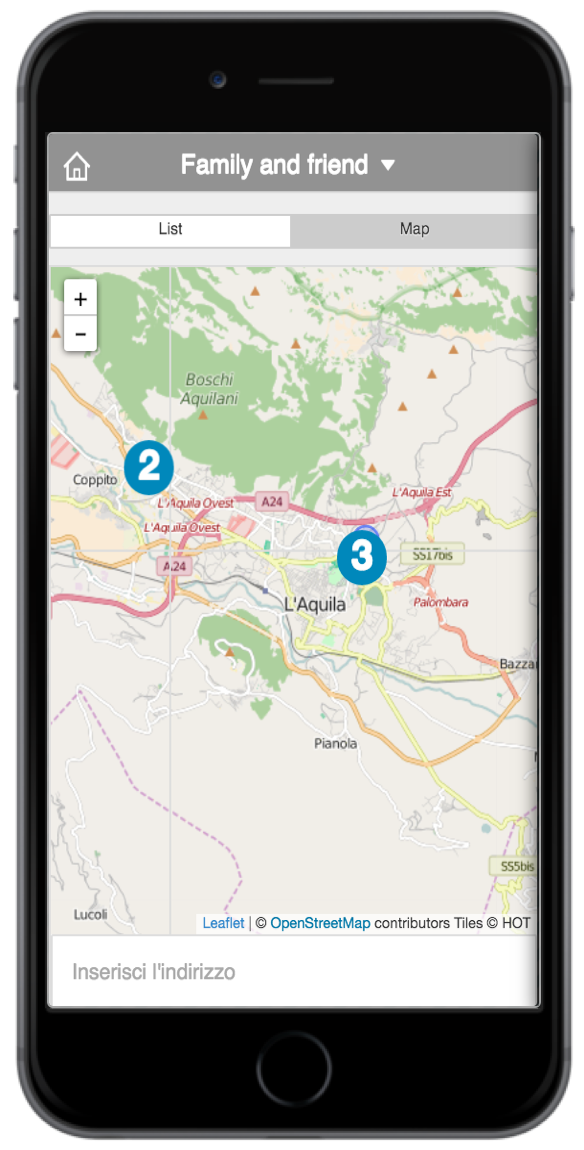
\includegraphics[scale=0.6]{interfaccia/markercluster.png}
	\caption{Due markercluster contenenti rispettivamente due e tre FOI }
	\label{fig:markercluster}
 \end{minipage}
 \ \hspace{6 mm} \hspace{7 mm} \
 \begin{minipage}[b]{6cm}
\centering
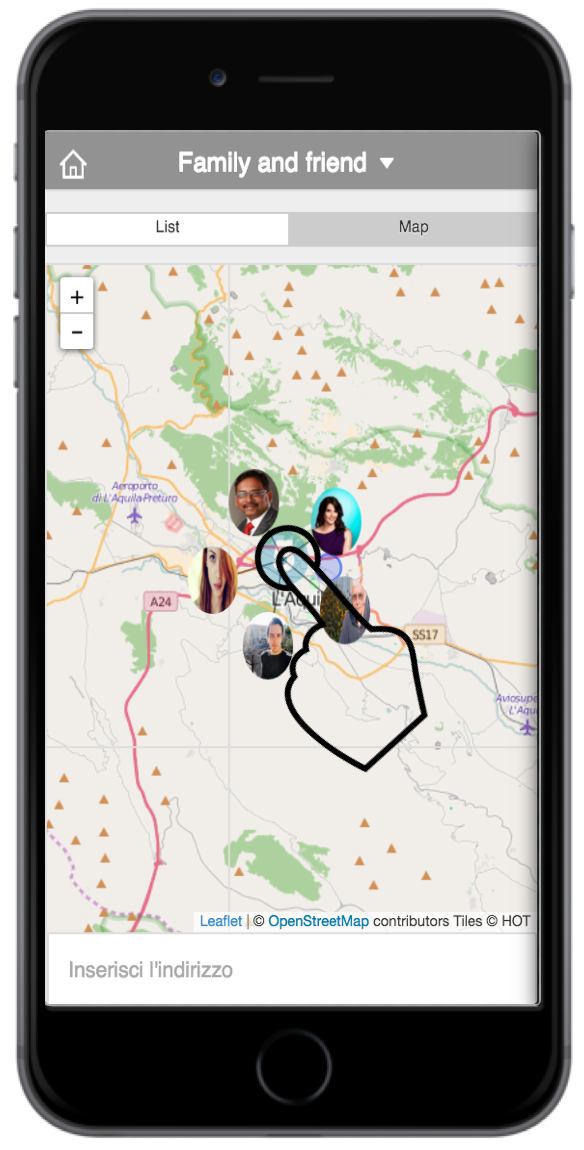
\includegraphics[scale=0.6]{interfaccia/markerfoi.png}
	\caption{Tap su un markercluster contenente cinque FOI }
	\label{fig:markerfoi}
 \end{minipage}
\end{figure}

 \begin{figure}
\textbf{POI:} le modalità di interazione e le schermate sono analoghe a quelle viste per i FOI. Per accedere alla lista (Fig \ref{fig:poilist}), bisogna cliccare sul bottone in fondo alla dashboard, come mostrato in Fig \ref{fig:buttonpoi}.
 \\ \\
 \begin{minipage}[b]{6cm}
   \centering
	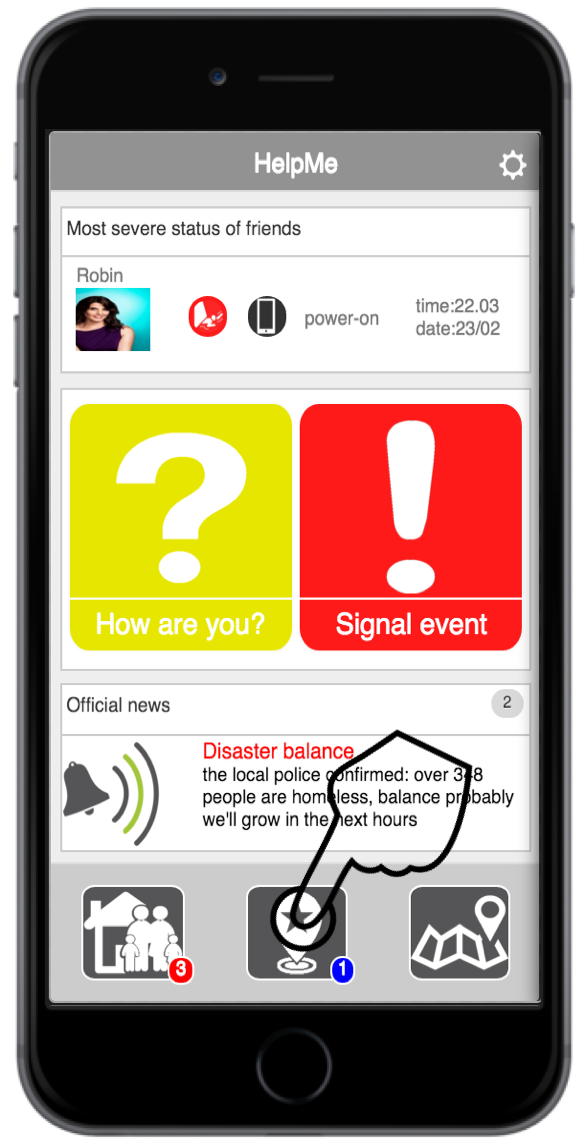
\includegraphics[scale=0.6]{interfaccia/buttonpoi.png}
	\caption{Tap da fare per accedere ai propri POI }
	\label{fig:buttonpoi}
 \end{minipage}
 \ \hspace{6 mm} \hspace{7 mm} \
 \begin{minipage}[b]{6cm}
\centering
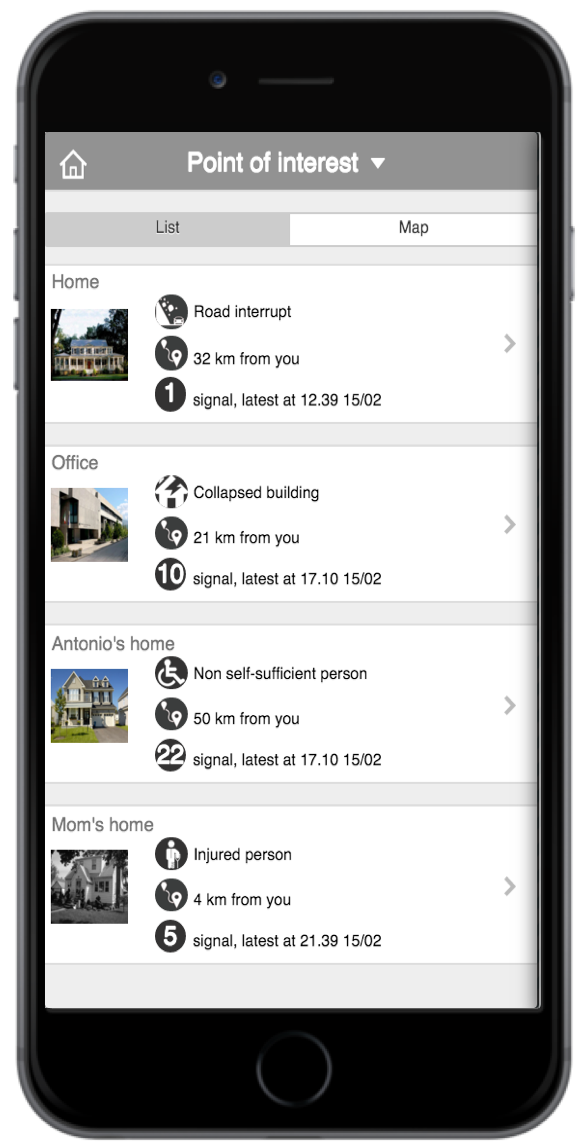
\includegraphics[scale=0.6]{interfaccia/poilist.png}
	\caption{Lista dei POI ordinata per default in base al più recente }
	\label{fig:poilist}
 \end{minipage}
\end{figure}

 \begin{figure}
\textbf{ POI:} Tappando su un marker, indipendetemente che sia un FOI o un POI, è possibile visualizzare le informazioni principali (Fig \ref{fig:tapmarker}). 
 \\ \\
 \begin{minipage}[b]{6cm}
   \centering
	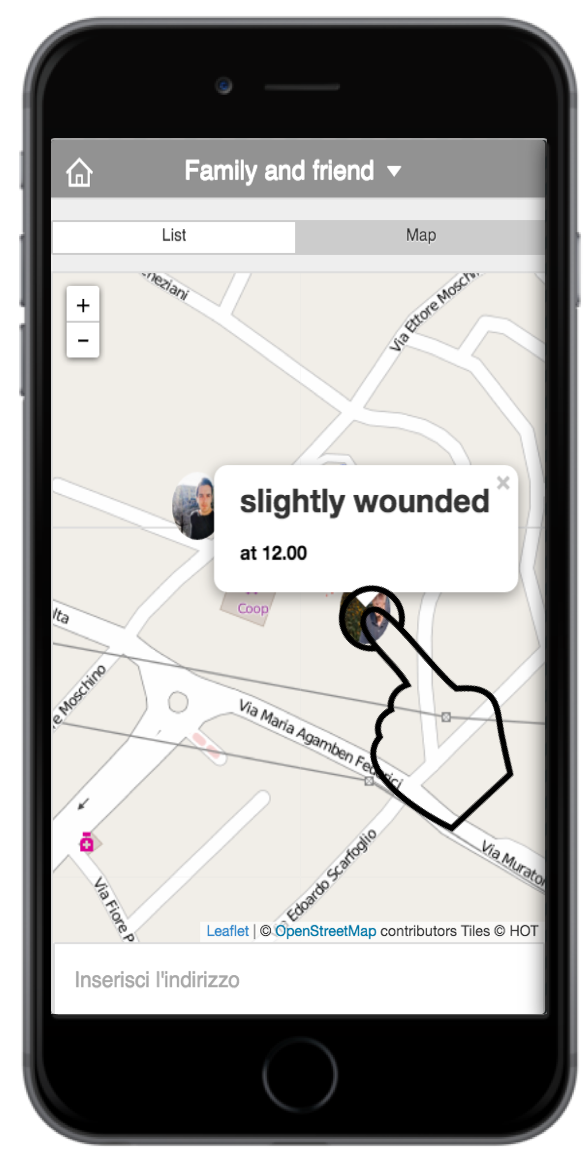
\includegraphics[scale=0.6]{interfaccia/tapmarker.png}
	\caption{Tap sul marker di un FOI }
	\label{fig:tapmarker}
 \end{minipage}
 \ \hspace{6 mm} \hspace{7 mm} \
 \begin{minipage}[b]{6cm}
\centering
\includegraphics[scale=0.6]{interfaccia/tappoimarker.png}
	\caption{Tap sul marker di un POI }
	\label{fig:poilist}
 \end{minipage}
\end{figure}





	


%\chapter{Implementazione}
\label{implementazione}
In questo capitolo vengono illustrati i dettagli implementativi riguardanti le realizzazioni hardware e software del sistema realizzato nell'ambito di questa tesi.

\section{Implementazione Hardware}
In questa sottosezione verrà mostrato inizialmente uno schema con i componenti hardware utilizzati per realizzare il sistema ideato in sez.\ref{descrizioeDelLavoro}, per finire verranno illustrati i canali di comunicazione.
\subsection{Schema hardware del sistema}
Con riferimento alla rappresentazione astratta del sistema a moduli presentata nella sez.\ref{livello_moduli}, segue una il medesimo schema ad un livello meno astratto nel quale si mostrano le componenti hardware che costituiscono i due moduli App e microcontrollore.
\begin{sidewaysfigure}[htbp]
	\includegraphics[width=\textwidth]{implementazione/schemaHardware.png}
	\caption{Schema hardware del sistema}
	\label{fig:schemaHardware}
\end{sidewaysfigure}
\newpage
Dove:
\begin{itemize}
	\item \textbf{Il modulo APP}: è composto da un'elaboratore nel quale si utilizzano i seguenti software
	\begin{itemize}
	\item \textit{RealTerm} per catturare in un file di log i dati inviati dal moduli microcontrollore
	\item \textit{Matlab} per testare l'algoritmo di \textit{Sensor Fusion} ed effettuare le varie analisi (sez.\ref{analisi})
	\end{itemize}
	\item \textbf{Il modulo Microcontrollore}: è composto da
	\begin{itemize}
		\item Una board Olimex con microcontrollore STM32F405 prodotto da \textit{STM}
		\item Un'unità di misura inerziale LSM9DS1 prodotta da \textit{STM}
	\end{itemize}
\end{itemize}
E' necessario spendere due parole a riguardo dell'implementazione del modulo APP mostrata in Fig.\ref{fig:schemaHardware}. \\
Relativamente al contesto applicativo individuato per questo sistema (sez.\ref{contesto}) l'applicativo Matlab e, più in generale, l'elaboratore non sono adatti alla realizzazione di un sistema IPS real-time. Tuttavia nel lavoro di questa tesi, questi vengono utilizzati al solo fine di comparare l'algoritmo di \textit{Sensor fusion} implementato (sez.\ref{sensor_fusion}) con quello eseguito all'interno del microcontrollore e di effettuare ulteriori analisi (sez.\ref{analisi}). Le fasi successive dello sviluppo di questo sistema, prevedono infatti lo studio della realizzazione ottima del modulo APP a partire dai risultati ottenuti dal lavoro di questa tesi.


\subsection{Canali di comunicazione}
In questa sezione verranno illustrati i canali di comunicazione (mostrati in Fig.\ref{fig:schemaHardware}) utilizzati per la trasmissione dei dati all'interno del sistema realizzato nell'ambito di questa tesi. Il primo paragrafo tratta il canale di comunicazione utilizzato tra il microcontrollore e l'unità di misura inerziale mentre nel secondo e ultimo paragrafo il canale di comunicazione utilizzato per trasmettere dati dal microcontrollore all'applicativo terminale sull'elaboratore.
\subsubsection{I2C}
\label{imp_i2c}
Per la comunicazione tra l' \textbf{IMU} e il \textbf{Microcontrollore}, si è utilizzato un canale di comunicazione seriale bifilare noto come \textit{Inter Integrated Circuit}, abbreviato \textbf{I2C}, come mostrato dalla seguente figura:
\begin{figure}[H]  
	\centering 
	\includegraphics[scale=0.1]{implementazione/i2cFoto.jpg}
	\caption{Foto del canale di comunicazione I2C tra il microcontrollore e l'unità di misura inerziale.}
	\label{fig:i2cFoto}
\end{figure}
Il protocollo \cite{i2cWiki} dell'I2C richiede due linee seriali per comunicare correttamente:
\begin{itemize}
	\item SDA (\textit{Serial Data}) per i dati
	\item SCL (\textit{Serial Clock}) per sincronizzare i dispositivi
\end{itemize}
Vanno inoltre aggiunte una connessione di riferimento alla massa e una alla linea di alimentazione (tipicamente 5 o 3,3 V) a cui sono connessi resistori di \textit{pull-up}, come mostrato dalla figura seguente:
\begin{figure}[H]  
	\centering 
	\includegraphics[scale=0.6]{implementazione/i2c.png}
	\caption{Rappresentazione di dispositivi collegati mediante I2C}
	\label{fig:i2c}
\end{figure}
L'I2C utilizza un indirizzo a 7 bit per un totale di 128 indirizzi disponibili. Poiché di questi 16 sono riservati, si ha un totale finale di 112 dispositivi collegabili alla medesima linea.\\
La velocità è il grande limite di questa comunicazione, infatti con le recenti revisioni si è riuscita a raggiungere una velocità massima di 3,4 Mbit/s (detto anche \textit{High Speed Mode}). Nello specifico di questa tesi lo si è utilizzato in \textit{fast mode} che corrisponde ad una velocità di 400 Kbit/s.\\
I dispositivi collegati al bus possono essere di due tipi:
\begin{itemize}
	\item Un \textit{Master} che controlla la SCL, inizializza le comunicazioni e invia dati
	\item Uno o più \textit{Slave} che rispondono ad un master e inviano dati
\end{itemize}

Il messaggio viene spezzato in due parti:
\begin{itemize}
	\item \textit{Address frame} dove il \textit{master} indica l'indirizzo dello \textit{slave} interessato alla comunicazione
	\item uno o più \textit{Data frames} contenenti l'informazione da trasmettere
\end{itemize}
I dati sono "piazzati" sulla linea SDA dopo che la linea SCL è posta a zero dal master, questi dati verranno letti dal dispositivo specificato nell'\textit{address frame} quando il \textit{master} riporterà la linea SCL al valore alto.\\
Relativamente al lavoro di questa tesi si identificano il \textit{Microcontrollore} come \textit{master} mentre l'\textit{IMU} come \textit{slave}. Nello specifico la comunicazione consiste nella lettura periodica da parte del microcontrollore dei valori misurati dai sensori all'interno dell'IMU. Tale lettura è stata realizzata leggendo i singoli registri ad 8 bit dei sensori (per maggiori dettagli si veda la stima temporale in sez.\ref{analisiTemporale}) attraverso lo script in Appendice \ref{scriptXLGRead} e rappresentato dalla seguente figura:
\begin{figure}[H]  
	\centering 
	\includegraphics[scale=0.5]{implementazione/i2cRead.png}
	\caption{Rappresentazione del flusso di dati generato per la lettura, tramite I2C, di un registro ad 8 bit.}
	\label{fig:i2cRead}
\end{figure}
Dove:
\begin{itemize}
	\item  \textit{ST} è il segnale di inizio di una comunicazione
	\item \textit{SAD + W} include l'indirizzo del dispositivo slave mentre l'ultimo bit specifica che il master sta per scrivere
	\item \textit{SAK} lo slave con l'indirizzo specificato precedentemente risponde con un segnale di \textit{acknowledge}
	\item \textit{SUB} è l'indirizzo del registro interno del dispositivo specificato precedentemente
	\item \textit{SAK} lo slave risponde con un segnali di \textit{acknowledge} se l'indirizzo del registro esiste
	\item \textit{SR} è il bit di ripetizione dello start utilizzato in combinazione con SAD+R/W
	\item \textit{SAD + R} include l'indirizzo del dispositivo slave mentre l'ultimo bit specifica che il master vuole ricevere dati
	\item \textit{SAK} segnale di \textit{acknowledge} da parte dello \textit{slave}
	\item \textit{DATA} dati trasmetti nel formato ad 8 bit
	\item \textit{NMAK} segnale di  \textit{non acknowledge} da parte del \textit{master}
	\item \textit{SP} bit di stop della comunicazione
\end{itemize}
Tuttavia questa lettura non è sempre la migliore, infatti è possibile continuare a leggere i registri interni dello \textit{slave} trasmettendo il segnale di \textit{MAK} invece del segnale di \textit{NMAK} mostrato in Fig.\ref{fig:i2cRead}. In questo modo l'IMU incrementerà l'indirizzo del registro interno di partenza specificato in \textit{SUB} e provvederà a trasmettere il valore del registro interno successivo ad esso. Questa funzionalità è molto utile quando si devono leggere dati, come in questo caso, che sono rappresentati con più registri. Così facendo infatti si riduce l'\textit{overhead} della trasmissione e si migliora quindi il goodput generale rispetto alla lettura ripetuta dei singoli registri.\\



\subsubsection{USB CDC}
\label{imp_usbcdc}
Per la comunicazione tra il \textit{microcontrollore} e l'elaboratore si è utilizzato un canale di comunicazione USB nella classe CDC \cite{usbCDC}, mostrato in Fig.\ref{usbFoto}, attraverso la libreria \textit{HAL} \cite{hal} fornita da \textit{STM}.
\begin{figure}[H]  
	\centering 
	\includegraphics[scale=0.1]{implementazione/usbFoto.jpg}
	\caption{Foto del canale di comunicazione USB usato nella classe CDC per la trasmissione dei dati dal microcontrollore all'elaboratore.}
	\label{fig:usbFoto}
\end{figure}
Un dispositivo CDC è composto \cite{usbCDC2} dalle seguenti interfacce:
\begin{itemize}
	\item \textit{Communications Class Interface} (CCI)
	\item \textit{Data Class Interface} (DCI)
\end{itemize}
L'interfaccia CCI è responsabile della gestione del dispositivo e in alcuni casi anche della gestione delle chiamate. Per gestione del dispositivo si intendono le configurazioni necessarie da eseguire sul \textit{device} e la notifica degli eventi, mentre per gestione della chiamata si intendono le operazioni necessarie per stabilire e terminare una comunicazione. La CCI è obbligatoria per tutti i dispositivi CDC in quanto lo identifica specificando il modello di comunicazione supportato dal dispositivo stesso.\\
L'interfaccia DCI è responsabile della trasmissione dei dati, infatti i dati trasmessi e/o ricevuti non seguono uno specifico formato. Tutte le interfacce di questo tipo possono essere viste come interfacce subordinate della CCI.\\
Tutti i dispositivi CDC devono avere almeno un'interfaccia CCI e zero o più interfacce DCI. Un CCI e ogni suo DCI subordinato forniscono una specifica funzionalità al dispositivo.\\
In generale un \textit{device} CDC potrebbe supportare diverse funzionalità e quindi essere composto da diversi set di CCI e DCI, come mostrato dalla figura seguente:
\begin{figure}[H]  
	\centering 
	\includegraphics[scale=0.4]{implementazione/cdcDevice.png}
	\caption{Rappresentazione di un dispositivo CDC che supporta tre diverse funzionalità.}
	\label{fig:cdcDevice}
\end{figure}
Un dispositivo CDC solitamente usa le senguenti combinazioni di \textit{endpoints}:
\begin{itemize}
	\item Una coppia di \textit{endpoints} di controllo IN e OUT chiamate \textit{endpoint di default}.
	\item Un \textit{endpoint} opzionale chiamato \textit{bulk} o \textit{interrupt IN}
	\item Una coppia di \textit{bulk} o \textit{endpoints} IN e OUT asincroni
\end{itemize}
La tabella \ref{tab:endpoints} mostra gli usi dei differenti \textit{endpoints} sopracitati e da quale interfaccia sono utilizzati.
\begin{table}[H]
	\centering
	\label{tab:endpoints}
	\begin{tabular}{|c|c|c|c|}
		\hline
		\textbf{Endpoint}                          & \multicolumn{1}{l|}{\textbf{Direzione}}        & \multicolumn{1}{l|}{\textbf{Interfaccia}} & \textbf{Uso}                                                                                                                                                                   \\ \hline
		Control IN                                 & Device-\textgreater{}Host                      & CCI                                       & \begin{tabular}[c]{@{}c@{}}Richiesta standard \\ per l'enumerazione,\\ richiesta specifica della classe,\\ controllo del dispositivo e\\ controllo della chiamata\end{tabular} \\ \hline
		Control OUT                                & Host-\textgreater{}Device                      & CCI                                       & "..."                                                                                                                                                                          \\ \hline
		Interrupt o bulk IN                        & Device-\textgreater{}Host                      & CCI                                       & \begin{tabular}[c]{@{}c@{}}Notifica di un evento\\ come lo stato della linea \\ o della rete\end{tabular}                                                                      \\ \hline
		\multicolumn{1}{|l|}{Bulk o OUT asincrono} & \multicolumn{1}{l|}{Host-\textgreater{}Device} & DCI                                       & \begin{tabular}[c]{@{}c@{}}Comunicazione di \\ dati grezzi o formattati\end{tabular}                                                                                           \\ \hline
		Bulk o IN asincrono                        & Host-\textgreater{}Device                      & DCI                                       & "..."                                                                                                                                                                          \\ \hline
	\end{tabular}
	\caption{Tabella con gli usi tipici degli \textit{endpoints} per comunicazioni USB-CDC}
\end{table}
La libreria HAL utilizzata nel lavoro di questa tesi, utilizza due tipi di \textit{endpoints} per la comunicazione:
\begin{itemize}
	\item \textit{Endpoint Bulk} per il trasferimento dei dati (1 \textit{endpoint} di OUT e 1 \textit{endpoint} di IN)
	\item \textit{Endpoint interrupt} per il controllo della comunicazione (richieste CDC, 1 \textit{endpoint} IN)
\end{itemize}
Il trasferimento dei dati IN (dal \textit{device} verso l'\textit{host}) è gestito periodicamente in base alle richieste dell'\textit{host} (il \textit{device} specifica l'intervallo di tempo tra le richieste dei pacchetti). Per questo motivo, un buffer statico circolare viene usato per memorizzare i dati mandati dal terminale del \textit{device} (esempio USART nel caso di una \textit{Virtual COM Port}).\\
In generale, la comunicazione USB è molto più veloce dell'output del terminale (ad esempio il bitrate massimo di un USART è tipicamente 115 Kbps mentre il bitrate dell'USB 1.1 è 12 Mbps in \textit{Full speed mode} o 480 Mbps in \textit{High speed mode}). Di conseguenza, prima di mandare nuovi pacchetti l'\textit{host} deve aspettare finché il \textit{device} non termina di processare i dati precedentemente inviati. Quindi, nel caso di data OUT dall'\textit{host} verso il \textit{device} l'uso di un buffer statico circolare non avrebbe senso. Il driver sul \textit{device} aspetta che la procedura di processamento del dato precedente sia terminata prima di mandare un segnale di \textit{acknowledge} all'\textit{host}. \\
Infine la gestione delle richieste di controllo viene effettuata utilizzando o un \textit{endpoint} pari a zero oppure attraverso un \textit{endpoint interrupt} infatti se la dimensione del pacchetto di richiesta non eccede i 64 bytes, allora l'\textit{endpoint 0} è sufficiente a gestire tale richiesta. 






\section{Implementazione Software}
In questa sezione si mostrano alcuni dettagli riguardanti l'implementazione software. Nella parte iniziale si fornisce un \textit{overview} delle funzionalità dei due moduli (sez.\ref{livello_moduli}) mentre nell'ultima parte si mostrano le modalità operative identificate e realizzate.
\subsection{Diagramma Comportamentale}
Per una avere una visione generale delle funzionalità implementate nei moduli APP e microcontrollore, si mostrano due pseudo diagrammi di flusso che ne sintetizzano il comportamento di ciascuno dei due.
\subsubsection{Diagramma del Microcontrollore}
Il comportamento del modulo Microcontrollore può essere rappresentato mediante il seguente diagramma di flusso:
\begin{figure}[H]  
	\centering 
	\includegraphics[scale=0.3]{implementazione/diagramma.png}
	\caption{Rappresentazione del comportamento per il modulo Microcontrollore.}
	\label{fig:diagrammaMicro}
\end{figure}
Dove:
\begin{itemize}
	\item \textbf{Init}: rappresenta la fase di inizializzazione del micro. L'utente sceglie la \textit{Computation Mode} e il numero di sensori da utilizzare (6DOF o 9DOF) modificando semplicemente due variabili globali (si veda appendice \ref{app:init}).
	\item \textbf{Start?}: il microcontrollore attende che il pulsante, integrato nella board, venga premuto di iniziare qualsiasi operazione.
	\item \textbf{LCM mode? e TCM mode?}: test di condizione sulla variabile globale che indica la \textit{Computation Mode} settata nella fase di inizializzazione. In base al suo valore il micro entrerà in un loop infinito della modalità scelta.
	\item \textbf{LCM}: procedura di \textit{Low Computation Mode}, sez.\ref{lcm}.
	\item \textbf{TCM}: procedura di \textit{Test Computation Mode}, sez.\ref{tcm}.
	\item \textbf{HCM}: procedura di \textit{High Computation Mode}, sez.\ref{hcm}.
	\item \textbf{Flag?}: test di condizione su una variabile di flag, modificata periodicamente da una routine tramite interrupt service.
\end{itemize}


\subsubsection{Diagramma del modulo APP}
Il comportamento del modulo APP relativo alla modalità \textbf{TCM} (sez.\ref{tcm}) può essere rappresentato mediante il seguente diagramma di flusso:
\begin{figure}[H]  
	\centering 
	\includegraphics[scale=0.4]{implementazione/diagrammaApp.png}
	\caption{Rappresentazione del comportamento per il modulo Microcontrollore.}
	\label{fig:diagrammaAPP}
\end{figure}
Dove:
\begin{itemize}
	\item \textbf{Init}: rappresenta la fase di inizializzazione della procedura. Vengono inizializzate le costanti necessarie all'algoritmo di sensor fusion (sez.\ref{sensor_fusion}), la variabile globale che definisce l'uso a 6DOF o 9DOF e infine i grafici da plottare successivamente.
	\item  \textbf{Read}: rappresenta la fase di lettura dei dati trasferiti dal modulo microcontrollore e salvati in un file di log. Ogni riga del file, corrispondente ad un pacchetto TCM (sez.\ref{tcm}), viene estratta e parsificata scomponendo la stringa in base ai separatori e i delimitatori utilizzati. Alla fine di questa fase si ottiene una matrice con i dati collezionati, per ogni sensore utilizzato, e una matrice con le stime dell'assetto elaborate dal microcontrollore.
	\item \textbf{Sensor Fusion}: rappresenta la fase di esecuzione dell'algoritmo di sensor fusion implementato (sez.\ref{descrizioneAlgoritmo}) a partire dalle matrici dei dati grezzi ottenuti nella fase precedente.
	\item \textbf{Plot stime}: vengono visualizzati gli angoli stimati dal microcontrollore e dal modulo APP al fine di completare l'analisi qualitativa dei due metodi (sez.\ref{analisiQualitativa})
\end{itemize}
Per i dettagli implementativi si rimanda alla lettura dell'Appendice \ref{app:tcmMatlab}.

\subsection{Modalità di computazione}
\label{computationMode}
In questa sezione verranno illustrate le modalità computazionali implementate all'interno del sistema (sez.\ref{livello_moduli}) e i relativi pacchetti dati utilizzati.

\subsubsection{Low Computation mode}
\label{lcm}
Questa modalità ha lo scopo di alleggerire il carico computazionale del microcontrollore, da qui il nome di \textit{low computation}. Infatti selezionandola l'algoritmo di \textit{sensor fusion}, per la stima dell'assetto (sez.\ref{sensor_fusion}), verrà eseguito dal modulo App, lasciando al microcontrollore la sola responsabilità di recuperare le misure effettuate dai sensori dell'IMU.\\
In questa modalità il pacchetto di dati da trasferire dal microcontrollore al modulo App ha la seguente struttura per la versione a 6DOF (giroscopio + accelerometro):
\begin{figure}[H]  
	\centering 
	\includegraphics[scale=0.5]{implementazione/lcm6Foto.png}
	\caption{Rappresentazione del pacchetto dati utilizzato in \textit{Low Computation Mode} a 6DOF}
	\label{fig:lcm6Foto}
\end{figure}
Con riferimento alla Fig.\ref{fig:lcm6Foto}, si mostra la tabella riepilogativa dei singoli campi:
\begin{table}[H]
	\label{tab:packlcm6dof}
	\begin{tabular}{|c|c|c|c|}
		\hline
		\textbf{Campo}    & \textbf{\begin{tabular}[c]{@{}c@{}}Formattazione\\ dati\end{tabular}} & \textbf{\begin{tabular}[c]{@{}c@{}}Dimensione\\ (bytes)\end{tabular}} & \textbf{Descrizione}                                                                                            \\ \hline
		Accelerometro - X & x,xxx                                                                 & 5                                                                     & \begin{tabular}[c]{@{}c@{}}Accelerazione misurata \\ lungo l'asse X\end{tabular}                                \\ \hline
		Accelerometro - Y & y,yyy                                                                 & 5                                                                     & \begin{tabular}[c]{@{}c@{}}" " \\ lungo l'asse Y\end{tabular}                                 \\ \hline
		Accelerometro - Z & z,zzz                                                                 & 5                                                                     & \begin{tabular}[c]{@{}c@{}}" "\\ lungo l'asse Z\end{tabular}                                 \\ \hline
		$\mid$             & \multicolumn{1}{l|}{}                                                 & 1                                                                     & \begin{tabular}[c]{@{}c@{}}Delimitatore tra i dati \\ dell'accelerometro\\ e quelli del giroscopio\end{tabular} \\ \hline
		Giroscopio - X    & xxx,xxx                                                               & 7                                                                     & \begin{tabular}[c]{@{}c@{}}Velocità angolare\\ misurata attorno  all'asse X\end{tabular}                        \\ \hline
		Giroscopio - Y    & yyy,yyy                                                               & 7                                                                     & \begin{tabular}[c]{@{}c@{}}" "\\ misurata attorno  all'asse Y\end{tabular}                        \\ \hline
		Giroscopio - Z    & zzz,zzz                                                               & 7                                                                     & \begin{tabular}[c]{@{}c@{}}" "\\ misurata attorno  all'asse Z\end{tabular}                        \\ \hline
		LF                &                                                                       & 1                                                                     & \begin{tabular}[c]{@{}c@{}}Carattere ASCII per la \\ codifica del comando\\ "nuova riga"\end{tabular}           \\ \hline
	\end{tabular}
	\caption{Tabella riepilogativa dei campi presenti nel pacchetto dati in LCM a 6DOF}
\end{table}
A questi vanno aggiunti quattro campi ";"  utilizzati per separare le varie misure assiali dei sensori.\\
Sommando le dimensioni massime dei singoli campi mostrati in tab.\ref{tab:packlcm6dof} si ottiene facilmente che la dimensione massima del pacchetto dati nella modalità \textit{Low Computation} a 6DOF è di \textbf{42 bytes}.\\
Nell'uso a 9DOF viene aggiunto un campo per i dati provenienti dal magnetometro (sez.\ref{magnetometro}), ottenendo la seguente struttura:

\begin{figure}[H]  
	\centering 
	\includegraphics[scale=0.4]{implementazione/lcm9Foto.png}
	\caption{Rappresentazione del pacchetto dati utilizzato in \textit{Low Computation Mode} a 9DOF}
	\label{fig:lcm9Foto}
\end{figure}

Con riferimento alla Fig.\ref{fig:lcm9Foto}, si mostra la tabella riepilogativa dei singoli campi:

\begin{table}[H]
	\begin{tabular}{|c|c|c|c|}
		\hline
		\textbf{Campo}    & \textbf{\begin{tabular}[c]{@{}c@{}}Formattazione\\ dati\end{tabular}} & \textbf{\begin{tabular}[c]{@{}c@{}}Dimensione\\ (bytes)\end{tabular}} & \textbf{Descrizione}                                                                                  \\ \hline
		Accelerometro - X & x,xxx                                                                 & 5                                                                     & \begin{tabular}[c]{@{}c@{}}Accelerazione misurata \\ lungo l'asse X\end{tabular}                      \\ \hline
		Accelerometro - Y & y,yyy                                                                 & 5                                                                     & \begin{tabular}[c]{@{}c@{}}Accelerazione misurata\\ lungo l'asse Y\end{tabular}                       \\ \hline
		Accelerometro - Z & z,zzz                                                                 & 5                                                                     & \begin{tabular}[c]{@{}c@{}}Accelerazione misurata\\ lungo l'asse Z\end{tabular}                       \\ \hline
		$\mid$            & \multicolumn{1}{l|}{}                                                 & 1                                                                     & \begin{tabular}[c]{@{}c@{}}Delimitatore tra i dati \\ dei sensori\end{tabular}                        \\ \hline
		Giroscopio - X    & xxx,xxx                                                               & 7                                                                     & \begin{tabular}[c]{@{}c@{}}Velocità angolare\\ misurata attorno  all'asse X\end{tabular}              \\ \hline
		Giroscopio - Y    & yyy,yyy                                                               & 7                                                                     & \begin{tabular}[c]{@{}c@{}}Velocità angolare\\ misurata attorno  all'asse Y\end{tabular}              \\ \hline
		Giroscopio - Z    & zzz,zzz                                                               & 7                                                                     & \begin{tabular}[c]{@{}c@{}}Velocità angolare\\ misurata attorno  all'asse Z\end{tabular}              \\ \hline
		$\mid$            &                                                                       & 1                                                                     & \begin{tabular}[c]{@{}c@{}}Delimitatore tra i dati \\ dei sensori\end{tabular}                        \\ \hline
		Magnetometro- X   & x,xxx                                                                 & 5                                                                     & \begin{tabular}[c]{@{}c@{}}Intensità del campo\\ magnetico esterno\\ sull'asse X\end{tabular}         \\ \hline
		Magnetometro- Y   & y,yyy                                                                 & 5                                                                     & \begin{tabular}[c]{@{}c@{}}Intensità del campo\\ magnetico esterno\\ sull'asse Y\end{tabular}         \\ \hline
		Magnetometro- Z   & z,zzz                                                                 & 5                                                                     & \begin{tabular}[c]{@{}c@{}}Intensità del campo\\ magnetico esterno\\ sull'asse Z\end{tabular}         \\ \hline
		LF                &                                                                       & 1                                                                     & \begin{tabular}[c]{@{}c@{}}Carattere ASCII per la \\ codifica del comando\\ "nuova riga"\end{tabular} \\ \hline
	\end{tabular}
	\caption{Tabella riepilogativa dei campi presenti nel pacchetto dati in LCM a 9DOF}
\end{table}
Ancora una volta per determinare la dimensione totale del pacchetto, bisogna aggiungere i sei campi ";" che separano le varie misure assiali dei sensori. Così facendo si ottiene banalmente che la dimensione totale per la LCM in 9DOF è di \textbf{60 bytes}. Per i dettagli implementativi si rimanda alla lettura dell'appendice \ref{app:lcm}.

\subsubsection{High Computation mode}
\label{hcm}
Questa modalità permette di assegnare al microcontrollore anche il compito di stimare l'assetto utilizzando la libreria \textit{MotionFX} fornita da STM. Risulta evidente come questa modalità sia la duale della precedente (sez.\ref{lcm}) in quanto aumenta il carico computazionale del microcontrollore, da cui il nome \textit{High Computation}. \\
Analogamente a quanto fatto per la modalità LCM, si mostra la struttura del pacchetto da trasferire dal microcontrollore al modulo APP per questa modalità:

\begin{figure}[H]  
	\centering 
	\includegraphics[scale=0.4]{implementazione/hcmFoto.png}
	\caption{Rappresentazione del pacchetto dati utilizzato in \textit{High Computation Mode}}
	\label{fig:hcmFoto}
\end{figure}
Si noti che in questo caso non vi sono distinzioni tra le strutture dei pacchetti a 6DOF e 9DOF, infatti indipendentemente da quanti sensori verranno utilizzati il microcontrollore dovrà sempre stimare l'assetto e mandarlo sotto forma di \textit{roll}, \textit{pitch} e \textit{yaw} (sez.\ref{angoliEulero}) al modulo APP. Con riferimento alla fig.\ref{fig:hcmFoto} si mostra la tabella riepilogativa dei campi:

\begin{table}[H]
	\centering
	\begin{tabular}{|c|c|c|c|}
		\hline
		\textbf{Campo} & \textbf{\begin{tabular}[c]{@{}c@{}}Formattazione\\ dati\end{tabular}} & \textbf{\begin{tabular}[c]{@{}c@{}}Dimensione\\ (bytes)\end{tabular}} & \textbf{Descrizione}                                                                                  \\ \hline
		Yaw            & xxx,x                                                                 & 5                                                                     &  \begin{tabular}[c]{@{}c@{}}Stima angolo\\ di imbardata\end{tabular}                                                               \\ \hline
		Pitch          & yyy,y                                                                 & 5                                                                     & \begin{tabular}[c]{@{}c@{}}Stima angolo\\ di beccheggio\end{tabular}                                            \\ \hline
		Roll           & zzz,z                                                                 & 5                                                                     & \begin{tabular}[c]{@{}c@{}}Stima angolo\\ di rollio\end{tabular}                                           \\ \hline
		LF             &                                                                       & 1                                                                     & \begin{tabular}[c]{@{}c@{}}Carattere ASCII per la \\ codifica del comando\\ "nuova riga"\end{tabular} \\ \hline
	\end{tabular}
\caption{Tabella riepilogativa dei campi presenti nel pacchetto dati in HCM}
\end{table}
Aggiungendo i due campi ";" utilizzati per separare gli angoli stimati, si ottiene che la dimensione del pacchetto dati da trasferire dal microcontrollore al modulo APP è di \textbf{18 bytes}.
Si noti come in questa modalità, pur aumentando il carico computazionale richiesto dal microcontrollore, si abbattano le dimensioni del pacchetto da trasferire al numero minimo di bytes necessari per rappresentare le stime degli angoli d'assetto in modo significativo. Per i dettagli implementativi si rimanda alla lettura dell'appendice \ref{app:hcm}.

\subsubsection{Testing Computation mode}
\label{tcm}
Quest'ultima modalità è stata pensata appositamente al fine di realizzare l'analisi qualitativa dell'assetto stimato (sez.\ref{analisiQualitativa}). La si può considerare come una modalità ibrida tra l'HCM e la LCM viste precedentemente, infatti in questo caso il pacchetto da trasferire dal microcontrollore al modulo APP include sia le misure dei sensori sia la stima dell'assetto.\\
In questa modalità il pacchetto di dati da trasferire dal microcontrollore al modulo App ha la seguente struttura per la versione a 6DOF:
\begin{figure}[H]  
	\centering 
	\includegraphics[scale=0.4]{implementazione/tcm6Foto.png}
	\caption{Rappresentazione del pacchetto dati utilizzato in \textit{Test Computation Mode} a 6DOF}
	\label{fig:tcm6Foto}
\end{figure}

Con riferimento alla Fig.\ref{fig:tcm6Foto}, si mostra la tabella riepilogativa dei singoli campi:
\begin{table}[H]
	\centering
	\begin{tabular}{|c|c|c|c|}
		\hline
		\textbf{Campo}    & \textbf{\begin{tabular}[c]{@{}c@{}}Formattazione\\ dati\end{tabular}} & \textbf{\begin{tabular}[c]{@{}c@{}}Dimensione\\ (bytes)\end{tabular}} & \textbf{Descrizione}                                                                                  \\ \hline
		Accelerometro - X & x,xxx                                                                 & 5                                                                     & \begin{tabular}[c]{@{}c@{}}Accelerazione misurata \\ lungo l'asse X\end{tabular}                      \\ \hline
		Accelerometro - Y & y,yyy                                                                 & 5                                                                     & \begin{tabular}[c]{@{}c@{}}Accelerazione misurata\\ lungo l'asse Y\end{tabular}                       \\ \hline
		Accelerometro - Z & z,zzz                                                                 & 5                                                                     & \begin{tabular}[c]{@{}c@{}}Accelerazione misurata\\ lungo l'asse Z\end{tabular}                       \\ \hline
		$\mid$            & \multicolumn{1}{l|}{}                                                 & 1                                                                     & \begin{tabular}[c]{@{}c@{}}Delimitatore tra i dati \\ dei sensori\end{tabular}                        \\ \hline
		Giroscopio - X    & xxx,xxx                                                               & 7                                                                     & \begin{tabular}[c]{@{}c@{}}Velocità angolare\\ misurata attorno  all'asse X\end{tabular}              \\ \hline
		Giroscopio - Y    & yyy,yyy                                                               & 7                                                                     & \begin{tabular}[c]{@{}c@{}}Velocità angolare\\ misurata attorno  all'asse Y\end{tabular}              \\ \hline
		Giroscopio - Z    & zzz,zzz                                                               & 7                                                                     & \begin{tabular}[c]{@{}c@{}}Velocità angolare\\ misurata attorno  all'asse Z\end{tabular}              \\ \hline
		$\mid$            &                                                                       & 1                                                                     & \begin{tabular}[c]{@{}c@{}}Delimitatore tra i dati \\ dei sensori\end{tabular}                        \\ \hline
		Yaw               & xxx,x                                                                 & 5                                                                     & \begin{tabular}[c]{@{}c@{}}Stima angolo\\ di imbardata\end{tabular}                                   \\ \hline
		Pitch             & yyy,y                                                                 & 5                                                                     & \begin{tabular}[c]{@{}c@{}}Stima angolo\\ di beccheggio\end{tabular}                                  \\ \hline
		Roll              & zzz,z                                                                 & 5                                                                     & \begin{tabular}[c]{@{}c@{}}Stima angolo\\ di rollio\end{tabular}                                      \\ \hline
		LF                &                                                                       & 1                                                                     & \begin{tabular}[c]{@{}c@{}}Carattere ASCII per la \\ codifica del comando\\ "nuova riga"\end{tabular} \\ \hline
	\end{tabular}
\caption{Tabella riepilogativa dei campi presenti nel pacchetto dati in TCM a 6DOF}
\end{table}
Ancora una volta aggiungendo sei campi ";" utilizzati per separare le misure assiali e gli angoli stimati si ottiene che la dimensione del pacchetto per questa modalità a 6DOF è  \textbf{60 bytes}.\\
Nell'uso a 9DOF viene aggiunto un campo per i dati provenienti dal magnetometro (sez.\ref{magnetometro}), ottenendo la seguente struttura:
\begin{figure}[H]  
	\centering 
	\includegraphics[scale=0.35]{implementazione/tcm9Foto.png}
	\caption{Rappresentazione del pacchetto dati utilizzato in \textit{Test Computation Mode} a 9DOF}
	\label{fig:tcm9Foto}
\end{figure}
Con riferimento alla Fig.\ref{fig:tcm9Foto}, si mostra la tabella riepilogativa dei singoli campi:

\begin{table}[H]
	\centering
	\begin{tabular}{|c|c|c|c|}
		\hline
		\textbf{Campo}    & \textbf{\begin{tabular}[c]{@{}c@{}}Formattazione\\ dati\end{tabular}} & \textbf{\begin{tabular}[c]{@{}c@{}}Dimensione\\ (bytes)\end{tabular}} & \textbf{Descrizione}                                                                                  \\ \hline
		Accelerometro - X & x,xxx                                                                 & 5                                                                     & \begin{tabular}[c]{@{}c@{}}Accelerazione misurata \\ lungo l'asse X\end{tabular}                      \\ \hline
		Accelerometro - Y & y,yyy                                                                 & 5                                                                     & \begin{tabular}[c]{@{}c@{}}Accelerazione misurata\\ lungo l'asse Y\end{tabular}                       \\ \hline
		Accelerometro - Z & z,zzz                                                                 & 5                                                                     & \begin{tabular}[c]{@{}c@{}}Accelerazione misurata\\ lungo l'asse Z\end{tabular}                       \\ \hline
		$\mid$            & \multicolumn{1}{l|}{}                                                 & 1                                                                     & \begin{tabular}[c]{@{}c@{}}Delimitatore tra i dati \\ dei sensori\end{tabular}                        \\ \hline
		Giroscopio - X    & xxx,xxx                                                               & 7                                                                     & \begin{tabular}[c]{@{}c@{}}Velocità angolare\\ misurata attorno  all'asse X\end{tabular}              \\ \hline
		Giroscopio - Y    & yyy,yyy                                                               & 7                                                                     & \begin{tabular}[c]{@{}c@{}}Velocità angolare\\ misurata attorno  all'asse Y\end{tabular}              \\ \hline
		Giroscopio - Z    & zzz,zzz                                                               & 7                                                                     & \begin{tabular}[c]{@{}c@{}}Velocità angolare\\ misurata attorno  all'asse Z\end{tabular}              \\ \hline
		$\mid$            &                                                                       & 1                                                                     & \begin{tabular}[c]{@{}c@{}}Delimitatore tra i dati \\ dei sensori\end{tabular}                        \\ \hline
		Magnetometro- X   & x,xxx                                                                 & 5                                                                     & \begin{tabular}[c]{@{}c@{}}Intensità del campo\\ magnetico esterno\\ sull'asse X\end{tabular}         \\ \hline
		Magnetometro- Y   & y,yyy                                                                 & 5                                                                     & \begin{tabular}[c]{@{}c@{}}Intensità del campo\\ magnetico esterno\\ sull'asse Y\end{tabular}         \\ \hline
		Magnetometro- Z   & z,zzz                                                                 & 5                                                                     & \begin{tabular}[c]{@{}c@{}}Intensità del campo\\ magnetico esterno\\ sull'asse Z\end{tabular}         \\ \hline
		$\mid$            &                                                                       & 1                                                                     & \begin{tabular}[c]{@{}c@{}}Delimitatore tra i\\ dati dei sensori e\\ l'assetto stimato\end{tabular}   \\ \hline
		Yaw               & xxx,x                                                                 & 5                                                                     & \begin{tabular}[c]{@{}c@{}}Stima angolo\\ di imbardata\end{tabular}                                   \\ \hline
		Pitch             & yyy,y                                                                 & 5                                                                     & \begin{tabular}[c]{@{}c@{}}Stima angolo\\ di beccheggio\end{tabular}                                  \\ \hline
		Roll              & zzz,z                                                                 & 5                                                                     & \begin{tabular}[c]{@{}c@{}}Stima angolo\\ di rollio\end{tabular}                                      \\ \hline
		LF                &                                                                       & 1                                                                     & \begin{tabular}[c]{@{}c@{}}Carattere ASCII per la \\ codifica del comando\\ "nuova riga"\end{tabular} \\ \hline
	\end{tabular}
\caption{Tabella riepilogativa dei campi presenti nel pacchetto dati in TCM a 9DOF}
\end{table}
Infine aggiungendo otto campi ";" utilizzati per separare le misure assiali e gli angoli stimati si ottiene che la dimensione del pacchetto per questa modalità a 9DOF è  \textbf{78 bytes}.\\
Quindi la TCM a 9DOF risulta essere la modalità con il maggiore carico computazionale richiesto al microcontrollore e con la dimensione maggiore dei pacchetti da trasferire dal micro al modulo APP. Per i dettagli implementativi si rimanda alla lettura dell'appendice \ref{app:tcm}.



%\chapter{Conclusioni e prospettive future}
\label{conclusioni}
A seguito dell'analisi qualitativa effettuata (sez.\ref{analisiQualitativa}), l'azienda presso la quale è stata svolta questa tesi
 ha ritenuto il lavoro fatto più che soddisfacente riconoscendo di aver acquisito tramite esso un sistema in grado di stimare l'assetto di un operatore con un margine di errore non significativo ai fini dell'applicazione e di aver contribuito ad arricchire il know-how aziendale riguardante la stima dell'assetto.\\
A partire dal lavoro di questa tesi vi sono molte prospettive, alcune delle quali verranno affrontate da proposte di tesi future:
\begin{itemize}
	\item Ottimizzazione dell'operazione di lettura delle misure dall'unità di misura inerziale tramite I2C.
	\item Caratterizzazione degli zero-offset e loro compensazione nell'algoritmo di \textit{Sensor Fusion} implementato.
	\item Identificazione della soluzione ottima per la realizzazione del modulo App.
\end{itemize}

Una volta realizzato interamente il sistema ideato e descritto nel capitolo \ref{descrizioeDelLavoro}, si avrà uno strumento innovativo in grado di fornire un aiuto significativo agli operatori che si trovano ad affrontare situazioni d'emergenza di questo tipo; contribuendo a salvare più vite umane.



%\chapter*{Ringraziamenti}
\markboth{Ringraziamenti}{Ringraziamenti}
\addcontentsline{toc}{chapter}{Ringraziamenti}
\thispagestyle{empty}

Desidero ringranziare sentitamente il prof. Giovanni De Gasperis per i preziosi consigli e il tempo dedicatomi. Inoltre desidero ringraziare la prof.ssa Laura Tarantino per avermi proposto questo affascinante lavoro e per i suoi utili insegnamenti, i quali hanno contribuito significativamente alla mia attuale formazione professionale come ingegnere.\\
Inoltre desidero ringraziare i miei amici e la mia compagna per avermi supportato durante tutto il mio percorso. Infine dedico questo e tutti i miei futuri successi alla mia famiglia, il mio carburante, la mia unica variabile globale.


% BEGIN Bibliografia
%\begin{thebibliography}{99}
\addcontentsline{toc}{chapter}{Bibliografia}

\bibitem{context}
Towards a Better Understanding of Context and Context-Awareness
\author{Anind K. Dey, Gregory D. Abowd}
\url{ftp://ftp.cc.gatech.edu/pub/gvu/tr/1999/99-22.pdf}

\bibitem{gps}
Sistema di posizionamento globale
\url{https://it.wikipedia.org/wiki/Sistema_di_posizionamento_globale#cite_note-1}


\bibitem{IPS}
Indoor positioning system
\url{https://en.wikipedia.org/wiki/Indoor_positioning_system}

\bibitem{IPS2}
Progettazione e realizzazione di un Indoor Positioning System basato su geomagnetismo e sensor fusion
\url{http://amslaurea.unibo.it/12840/1/federico_torsello_tesi.pdf}

\bibitem{alg1}
Luca Pappalardo, "Localizzazione - Problema, Tecniche, Algoritmi - Reti mobili:
Ad Hoc e di sensori", 2011,
\url{http://didawiki.di.unipi.it/lib/exe/fetch.php/rhs/localizzazione.pdf}

\bibitem{alg2}
Cuccado, De Franceschi, Fauri, Sartor, "Analisi di algoritmi di autolocalizzazione
per reti di sensori wireless", 2007,
\url{https://art.torvergata.it/retrieve/handle/2108/773/6945/Paolo-Sperandio-Tesi-PhD.pdf}

\bibitem{indoorThesis}
An adaptive indoor positioning system based on Bluetooth Low Energy RSSI
\author{Nicola Cinefra}
\url{https://www.politesi.polimi.it/bitstream/10589/92284/3/NicolaCinefra770910TesiDefinitiva.pdf}

\bibitem{market}
Harrop P, Raghu D. Mobile Phone Indoor Positioning Systems (IPS) and Real Time
Locating Systems (RTLS) 2014-2024. Forecasts, Players, Opportunities. IDTechEx



\bibitem{rssi}
Ugur Bekcibasi, "Increasing RSSI Localization Accuracy with Distance Reference
Anchor in Wireless Sensor Networks", 2014,
\url{http://www.uni-obuda.hu/journal/Bekcibasi_Tenruh_54.pdf}

\bibitem{toaProblem}
Mak LC, Furukawa T. A ToA-based Approach to NLOS Localization Usiong Low-Frequency Sound. ACRA2006 (Auckland, New Zealand); 2006


\bibitem{aoa}
A Simple Technique for angle of arrival measurement
\url{https://www.researchgate.net/publication/4368716_A_Simple_Technique_for_angle_of_arrival_measurement}

\bibitem{triangolazione}
Generalized Geometric Triangulation Algorithm for Mobile Robot
Absolute Self-Localization 
\url{https://pdfs.semanticscholar.org/dee6/fb124433cac10744afd9502b165ffdecb202.pdf}

\bibitem{sensorfusion}
Sensor fusion
\url{https://en.wikipedia.org/wiki/Sensor_fusion}

\bibitem{mems}
Jeroen Hol "Sensor Fusion and Calibration of
Inertial Sensors, Vision,
Ultra-Wideband and GPS"
\url{https://www.xsens.com/wp-content/uploads/2014/pdf/Hol2011%20-%20Dissertation.pdf}

\bibitem{principimems}
Janusz Bryzek "Principles of MEMS"
\url{https://www.wiley.com/legacy/wileychi/hbmsd/pdfs/mm573.pdf}


\bibitem{acc}
MEMS Accelerometer
\url{http://www.instrumentationtoday.com/mems-accelerometer/2011/08/}


\bibitem{gyromodel}
H. Titterton and J. L. Weston. Strapdown inertial navigation technology. IEE
radar, sonar, navigation and avionics series. Peter Peregrinus Ltd., Stevenage,
UK, 1997. ISBN 0863413587.

\bibitem{corolois}
Forza di Coriolis, Wikipedia
\url{https://it.wikipedia.org/wiki/Forza_di_Coriolis}

\bibitem{gyroMems}
The Development of Micromachined Gyroscope Structure and
Circuitry Technology, Dunzhu Xia, Cheng Yu and Lun Kong

\bibitem{assetto}
TECNICHE DI STIMA E CONTROLLO DI ASSETTO DI
SATELLITI. Andrea Fagiani. 
\url{http://control.disp.uniroma2.it/carnevale/archivio/Tesi/andreafagianiM/tesi.pdf}




\bibitem{trackingThesis}
Advanced algorithms and architectures for MEMS inertial sensor platforms 
in orientation tracking and in fall detection applications. Simone Sabatelli.
Università di Pisa.

\bibitem{motion}
MotionFX middleware library in X-CUBE-MEMS1 software
expansion for STM32Cube.\\
\url{http://www.st.com/content/ccc/resource/technical/document/user_manual/group0/31/0e/66/39/cb/f7/4e/cd/DM00394369/files/DM00394369.pdf/jcr:content/translations/en.DM00394369.pdf}


\end{thebibliography}




% END Bibliografia


\end{document}